\documentclass[logo,magister,dosguias]{tesis-postgrado}
% opciones: logo,dosguias,magister,doctorado,propuesta,txfonts

\usepackage{blindtext}

%\keywords{SPS;Elasticidad;Algoritmo reactivo;Algoritmo predictivo}

\begin{document}
\baselineskip 23pt

\frontmatter %Utiliza numeración romana

% ----------------------------------------------------------
% ----------- PARTE INICIAL --------------------------------
\thispagestyle{empty}
\facultad{Ingeniería}
\departamento{Ingeniería Informática}
\grado{Magíster en Ingeniería Informática}

\titulo{Modelo elástico de replicación de operadores para un sistema de procesamiento de \textit{stream} en tiempo real}

\autor{Daniel Pedro Pablo Wladdimiro Cottet}
\email{daniel.wladdimiro@usach.cl}
\annoingreso{2014}

\fecha{Lunes}{21}{Septiembre}{2015}

\profesorguia{Nicolás Andrés Hidalgo Castillo}
\profesorcoguia{Erika Susana Rosa Olivos}

\ciudad{Santiago}
\pais{Chile}

\makecubierta


% ----------------------------------------------------------
% ----------- PRIMERA PARTE --------------------------------
% ### Resumen e Indices ####
\pagestyle{fancy}
\renewcommand{\headrulewidth}{0pt} %Hace que no aparezca la linea horizontal superior al principio de estas páginas
\fancyhead[L]{}
\fancyhead[C]{}
\fancyhead[R]{}


\makecopyright % si es propuesta no se mostrará

\dedicatoria{
Gracias a la vida que me ha dado tanto\\
Me ha dado la risa y me ha dado el llanto,\\
Así yo distingo dicha de quebranto\\
Los dos materiales que forman mi canto\\
Y el canto de ustedes que es el mismo canto\\
Y el canto de todos que es mi propio canto.
}

\begin{agradecimiento}
\small{Me cuesta encontrar las palabras para expresar lo que siento, se cierra un ciclo en mi vida, y con ello una larga traves\'ia de mucho esfuerzo y trabajo, donde espero que de inicio a muchos m\'as. Recib\'i apoyo, cari\~no y paciencia de diferentes personas, las cuales sub\'ian y bajaban de este exc\'entrico tren en cada parada que hac\'iamos, y aunque a veces entre paradas se hac\'ia un viaje muy corto, hab\'ian otras veces que se hac\'ian unos viajes eternos, y no terminaba de distinguir realmente bien d\'onde iba, pero eso daba igual, porque siempre en cada trayecto aprend\'ia y recib\'ia algo de alguna persona, y eso me hizo ir creciendo con el tiempo, lo cual estoy eternamente agradecido. De antemano pido disculpas si me he olvidado de alguien, no fue mi intenci\'on, y espero que pueda agradecerlo en un tiempo futuro. 

Aunque uno a veces siente que todo cambia; la gente, el barrio, la universidad, la sociedad, el trabajo, hay sentimientos y pasiones que nunca cambian, y son esas que te hacen vibrar y llenarte el coraz\'on por estar ah\'i. Sin duda alguna, Izquierda Libertaria es una mis grandes pasiones, donde a trav\'es del FeL me brind\'o una escuela de lucha para poder construir un pueblo digno y soberano. No saben como agradezco estar ah\'i y conocer a mis amigas y amigos que adem\'as son compa\~neras y compa\~neros de lucha: Thomi, Neto, Cachorro, Sussan, Andr\'es, Zarri, Cata, Pato, Cristi\'an, Tuto, Nati, Joaco, Fofi, de coraz\'on gracias por todo su apoyo incondicional. Y m\'as todav\'ia agradezco al FeL porque aqu\'i conoc\'i a mi amada polola, quien no s\'olo le agradezco su apoyo, sino tambi\'en por su cari\~no, alegr\'ia y paciencia, y sin duda todo ser\'ia muy distinto sin ti, no sabes lo agradecido y feliz que soy de estar con vos. Te amo Cami.

Cuando uno va viajando, vas creciendo, vas madurando, te vas dando cuenta que puedes ir resolviendo problemas que antes se hac\'ian imposibles, van d\'andose nuevas herramientas, nuevas habilidades. Por lo mismo es que estoy completamente agradecido de la oportunidad que me brindaron mis queridos profesores gu\'ias Erika y Nicol\'as, porque confiaron en m\'i y se la jugaron por sacar este trabajo, y no s\'olo eso, de abrirme puertas para poder sustentarme y tener un porvenir m\'as tranquilo. De verdad no saben lo orgulloso que estoy de tenerlos como profesores, no s\'olo me han ayudado a formarme como profesional, sino tambi\'en como persona y eso se los agradezco desde el fondo de mi coraz\'on. Tambi\'en agradezco a Pamela, por su apoyo y entrega incondiconal, y la profesora Carolina y el profesor Mauricio, que gracias a CITIAPS me sent\'i en mi segundo hogar, y siento que mucha de las cosas que aprend\'i hoy en d\'ia es gracias a esa peque\~na salita de gran coraz\'on. Y por lo mismo, no puedo olvidar a mi compa\~nero de trabajo, Pablo, siempre me acuerdo como nos conocimos en ese primer d\'ia de las clases de Mag\'ister, nunca cre\'i que gracias a ese saludo pudi\'eramos tener este viaje, donde sali\'o un paper, un proyecto y una bonita amistad, de verdad gracias Pablo, sos un hermano para m\'i. Gracias a todos los que pasaron y est\'an en CITIAPS, \'Alvaro, Jeff, Diego, Farisori, no me olvidar\'e de ustedes, porque sin duda me dejaron marcado y me ayudaron a formarme como profesional y persona. Tambi\'en a mis amigas y amigos de la Usach, Miguel, Gabo, Clau, Karla, Jorge, los quiero caleta y gracias por todo, porque fueron un pilar en mi vida universitaria, donde no los olvidar\'e, porque todo lo que viv\'i con ustedes fue una de mis grandes alegr\'ias.

Pero a veces uno se queda dormido, recuerdas el pasado, y te acuerda que eso fue lo que te form\'o y lo que explica el c\'omo eres hoy en d\'ia. Nunca los voy a olvidar, para mi son mi fuerza, mis ganas, mi apa\~ne, quiz\'a todos estamos en nuestras vidas, pero los tengo mas presente que nunca, Jos\'e, Eduardo, Rub\'en y Felipe, los quiero demasiado. Y como te voy a olvidar, si sos mi hermano de leche, Sim\'on, no s\'olo te tengo que agradecer, te deber\'ia hacer una oda por lo grande que has sido conmigo. Tantas cosas que pasamos, tanto que vivimos, tantos recuerdos, y como fuimos creciendo, donde sea que est\'es tengo claro que puedo contar contigo, y estoy seguro que t\'u sientes lo mismo de m\'i.

Y alguien tuvo que crear la primera estaci\'on del viaje, alguien tuvo que armar ese tren, y es algo que aunque suba y bajen mil personas, pasen mil a\~nos, nunca podr\'as borrarlo, y me alegro que sea as\'i, porque es lo m\'as valioso que uno tiene, la familia. Como no quererlas, si me mimaron, me criaron, me abrazaron, me apoyaron, y eso lo agradezco, a ti Amandi, a ti Sofi y a ti Mam\'a, las amo. Obvio, no me voy a olvidar de ti, gracias por todo tu apoyo Pap\'a, siento que mucho de lo que aprend\'i fue gracias a ti, y me alegro haber tenido esa oportunidad.

Agradezco tambi\'en al PMI-USA 1204 y al proyecto DICYT-USACH 061419HC por darme la tranquilidad de poder trabajar en este largo proyecto.}
\end{agradecimiento}


\pagestyle{fancy}
%\fancyhead[L]{\slshape \leftmark}


\tableofcontents        %% Indice general
\listoftables           %% Indice de tablas
\listoffigures          %% Indice de figuras
\listofalgorithms       %% Indice de algoritmos

\resumenCastellano{
En el mundo actual de la información, grandes cantidades de datos son generados cada segundo desde las más diversas fuentes: redes sociales, redes de sensores, buscadores Web, entre otros. Extraer información de dichos datos muchas veces requiere que este procesamiento sea llevado a cabo en tiempo real, debido a que el análisis que se debe realizar depende de la temporalidad en que son generadas los eventos. Para lograr procesar grandes cantidades de datos con estas restricciones, existen sistemas especializados llamado sistemas de procesamiento de \textit{stream} (SPS), los cuales pueden procesar en tiempo real los datos que van llegando por una o más fuentes de datos. Estos sistemas están basados en grafos, cuyos vértices realizan operaciones sobre un flujo de datos que va llegando reflejada por las aristas del grafo. La topología del grafo le brinda flexibilidad al SPS para generar \hl{diversas} aplicaciones de procesamiento, sin embargo, dicha topología es estática una vez el sistema se ejecuta. Dado este problema, este trabajo se plantea un modelo elástico que sea capaz de adaptar la topología del grafo a las condiciones del tráfico existente. Para esto se ha diseñado un algoritmo reactivo, usando la técnica de fisión, y otro predictivo, usando cadena de Márkov, ambas técnicas permiten estimar la carga de los operadores, y adaptar el grafo acorde a lo indicado por estos. Dicha modificación consiste en incrementar o disminuir la cantidad de réplicas de un operador según su nivel de carga. Los resultados obtenidos de los experimentos realizados en el SPS S4, muestran una mejora de hasta nueve veces más eventos procesados, con un costo asociado a un aumento de $0,01\%$ del uso de la CPU, pero una disminución de un $1,5\%$ en el consumo de memoria RAM.
\vspace*{0.5cm}
\KeywordsES{SPS; Elasticidad; Distribución de carga; Balance de carga; Algoritmos reactivos; Fisión; Algoritmos predictivos; Cadena de Márkov}
}

\newpage

\resumenIngles{
In the actual world of information, great quantities of data are generated every second from the most diverse sources: social networks, sensor networks, web searchers, among others. Extract information from that data requires a real-time process to be done due to the analysis that depends of the temporality in which the events are generated. To process this big quantity of data with this constraints, there are specialized systems called stream processing streams, which can process data from diverse sources in real time the data coming from one or more sources. This systems are based on graphs, which vertices operate depending of the incoming stream of data through their edges. This topology gives a certain flexibility to the SPS to generate diverse processing applications. However, this topology is static at the time that is executed. Given this problem, this work proposes an elastic model that is able to adapt the graph topology to the existing traffic conditions. A reactive algorithm have been designed for this, using the fission technique and a preactive one, using Markov chain, this two techniques allows to estimate de operators loads and to adapt the graph according of what they are indicating. This modification consists on increase and decrease the quantity of operator replicas depending of the load level. The obtained results from the experiments done in the SPS S4, show an improvement up to nine times more processed events, with an associated cost of $0.01\%$ if CPU use, but with a decrease of $1.5\%$ RAM consumption.
\vspace*{0.5cm}
\KeywordsEN{SPS; Elastic; Load balancing; Reactive Algorithm; Fision; Predictive Algorithm; Markov chain}
}



% ----------------------------------------------------------
% ----------- SEGUNDA PARTE --------------------------------
\mainmatter %Reinicia el contador de páginas para partir de 1 y usando números arábicos.
% ### Configuración del header ###
\pagestyle{fancy}
\renewcommand{\headrulewidth}{0.4pt} %Hace que vuelva a aparecer la linea horizontal
\fancyhead[LE,RO]{\slshape \leftmark} %Hace que se muestre el título del capítulo en las páginas que no son la primera de cada capítulo
%Comentar la linea anterior y descomentar la siguiente si se usa oneside:
%\fancyhead[L]{\slshape \leftmark}

% ### Capitulos de la tesis ###
\chapter{Introducción}
\label{cap:introduccion}

\section{Antecedentes y motivación}
\label{intro:motivacion}

La gran contribución de información en la Internet se ha debido al origen de la Web 2.0, donde ésta se caracteriza por la participación activa del usuario, siendo reflejado en el auge de blogs, redes sociales u otras aplicaciones web \citep{web2007oberhelman}. Con el objetivo de extraer información de dichos datos, se crean sistemas de procesamiento para grandes cantidades de información generadas por la interacción entre los usuarios.

Con el paso del tiempo, más y más información es generada por distintas interacciones generadas por los usuarios. Por lo que, analizar o extraer esta información no es una tarea fácil, más aún cuando muchas de estas interacciones deben ser analizadas en tiempo real, dada su dependencia temporal. Por lo que sistemas tradicionales de procesamiento basados en MapReduce \citep{2010Lin} o \textit{bash processing} \citep{HawwashN14} no son los ideales para analizar esta información.

Es así como con el tiempo se han ido creando distintas aplicaciones de procesamiento en tiempo real, debido al interesante funcionamiento que poseen, las que se caracterizan por ser capaces de procesar grandes flujos de datos en tiempo real \citep{ChenZ14a}. La necesidad de procesar informaci\'on en tiempo real surge dado que muchas aplicaciones, donde sus usuarios requieren de respuestas r\'apidas y actualizadas que le permitan tomar decisiones en per\'iodos cortos de tiempo. Dentro de los ejemplos existentes se encuentran; análisis de sentimientos de los mensajes de usuarios, análisis de los precios de la bolsa de valores, recopilación de información en caso de emergencia, entre otros. Las distintas aplicaciones que se han creado se volvieron críticas para sus usuarios, debido que sustenta la toma de decisiones de empresas o instituciones \citep{Wenzel14}.

Un ejemplo de esto, son las aplicaciones que analizan redes sociales en caso de un desastre natural, donde grandes cantidades de información son generadas, y se requiere procesar esta información lo más cercano al tiempo real para obtener información que sea relevante para la situación \citep{andrade2014fundamentals}. De esta manera, se puede construir un sistema que pueda procesar los datos realizando análisis de sentimiento, búsqueda de palabras claves o filtros de búsqueda, ya sea por idioma, país o género. Con esta información, se puede establecer sectores críticos, facilitar la búsqueda de personas, distribución de alertas, o detección de necesidades, lo cual sería crucial para tomar decisiones en esos momentos.

Por otra parte, también son utilizado estos sistemas de procesamiento para llevar a cabo predicciones en la bolsa de comercio, de esta manera, se crean sistemas de procesamiento que apliquen modelos matemáticos y permiten predecir el comportamiento para el siguiente día en el mercado. Con estos sistemas, la ganancia que existe por parte de las personas interesadas puede aumentar considerablemente, por lo que ha generando un alto interés en el desarrollo e investigación en esta área.

También se aplica en casos de seguridad, dado que se realiza un monitoreo de la actividad que surge por parte de los usuarios que interactúan en una red específica. Esto es útil para empresas o ministerios que poseen información privilegiada, y en caso que alguien desee realizar respaldos o eliminar información sin consentimiento de los encargados, puede detectarse la persona y generarse una alarma de preventiva a las autoridades. Como la información es procesada en tiempo real, ayuda a detectar a tiempo las posibles acciones de usuarios maliciosos. Dentro de las aplicaciones que existen sobre este tema, son los análisis de logs de los sistemas, con cuya información se puede verificar si existe algún \textit{bug}, error o anomalía, además de ver si existe algún intruso o violación al sistema.

Entre los sistemas actuales de procesamiento de \textsl{stream} se encuentran S4 \citep{s4yahoo}, Storm \citep{stormtwitter}, Samza \citep{samza}, entre otros, los cuales son los más utilizados como arquitectura de procesamiento en la confección de distintas aplicaciones de \textsl{stream}. Este tipo de arquitecturas está basada en grafos, donde las vértices son operaciones realizadas al flujo de datos que es enviado por las distintas aristas. Por lo que el usuario diseña la topología a su conveniencia, según la necesidad que posea el sistema, creando así una aplicación. Aunque poseen bastante flexibilidad para la creación de diversas aplicaciones, por la facilidad de crear distintas topologías, no lo tiene para adaptarse en el tiempo a las condiciones del tráfico entrantes, esto debido a que las topolog\'ias de procesamiento generadas son est\'aticas. Dada la naturaleza din\'amica de las interacciones, pueden surgir problemas de sobrecarga en algunas partes de la topología asociada a la aplicación.

El problema de sobrecarga conlleva a una baja en el rendimiento, produciendo una pérdida de recursos, tiempo e información. Abordar este problema es crítico, puesto que al realizar una optimización en el sistema, implica una disminución en el tiempo de procesamiento, por lo que hay una mayor cantidad de datos procesados en un período de tiempo, lo cual conlleva a una mayor precisión en los resultados obtenidos de la aplicación.

Lo anterior lo podemos entender de mejor manera con el siguiente ejemplo: se posee un tiempo $t$ para procesar $n$ datos, de disminuir el tiempo de procesamiento total de los datos, se tiene que en el mismo tiempo $t$ se procesarán una cantidad $n+m$ de datos, donde $m$ son los datos adicionales a analizar debido a la mejora del rendimiento. Como existe un aumento en la cantidad de datos procesados, la información procesada posee mayor precisión, debido que se poseen mayor cantidad de datos con los que analizar el comportamiento estudiando. Por ejemplo, al procesar una mayor cantidad de transacciones en la bolsa de comercio, se puede poseer una predicción más precisa de cómo se comportará la bolsa a futuro. Desde otro punto de vista, se efectúa una mejora en los recursos utilizados, habiendo una disminución de recursos ociosos que genera la sobrecarga en el operador.

\section{Descripción del problema}
\label{intro:problema}

%En los SPS (Sistemas de Procesamiento de \textit{Streaming}) son planteados como un grafo en el cual cada vértice es un operador y las aristas son el flujo de datos entre operadores. Debido a esto, puede generarse alguna sobrecarga del sistema, dado distintos factores, entre los cuales puede ser físico o lógico. El físico se define como los componentes que posea la máquina que generan una limitante en el sistema. En cambio, el lógico es una limitante dado los componentes del grafo generador por el sistema.

Los SPS (Sistemas de Procesamiento de \textit{Streaming}) modelan sus aplicaciones como un grafo cuyas vértices son operadores y las aristas son flujo de datos entre los operadores. Dada el carácter estático de su representación en forma de grafo, puede existir sobrecarga del sistema a producto de factores físicos o lógicos. El factor físico se define como los componentes que posee la máquina, los cuales pueden ser limitantes para el sistema alojado. En cambio, el lógico se concentra en los componentes del grafo, por lo que existe una limitante en la cantidad de operadores o la cantidad de flujo existente entre los operadores.

%Es por esto, que el problema se plantea como la sobrecarga que puede existir en el sistema debido a los distintos factores lógicos, como la cola de cada operador, siendo esto a causa de la falta de flexibilidad del SPS, en los operadores más demandados. Esto debido a que no existe una forma de disminuir la sobrecarga y reducir las colas de espera, para mejorar el rendimiento del sistema y obtener información cercana al tiempo real.

La falta de flexibilidad del SPS en los operadores más demandados. Esto sucede dada la condición estática del grafo, es decir la topología del grafo no cambia con el tiempo, por lo que no existe una forma para adaptarse el tráfico de manera dinámica que permita variar la carga y reducir las colas, de tal manera de mejorar el rendimiento del sistema y obtener información más precisa y en tiempo real.

\section{Solución propuesta}
\label{intro:solucion}

La solución propuesta consiste en el dise\~no de algoritmos de predicci\'on y distribuci\'on de carga a nivel de la l\'ogica del grafo, los cuales adaptan el grafo a las variaciones del grafo. Por lo que se propone implementar cuatro módulos que componen la estructura del sistema de distribución de carga: monitor de carga, analizador de carga, predictor de carga y administrador de réplicas.

El monitor de carga está encargado de recuperar el nivel de carga de cada uno de los operadores. Esta información es entregada a los módulos de analizador y predictor de carga, los cuales están encargados de evaluar si existe sobrecarga en el operador. Cada uno de éstos trabaja de forma independiente y tiene distintos métodos, uno proactivo y otro reactivo, de tal manera de poseer mayor exactitud en la detección de una sobrecarga.

El analizador de carga consiste en un método reactivo, el cual analiza el tráfico de los operadores en el tiempo actual, y cuantifica su carga. El estado de la carga de cada operador depende de un umbral, por lo que según ésto se envía al administrador de réplica el tráfico de cierto operador de ser necesario una replicación.

El predictor de carga consiste en un método proactivo, el cual analiza la carga de los distintos operadores según una ventana de tiempo, y predice la carga para la siguiente ventana de tiempo. De esta manera, se determina la posible carga que existe en cierto período de tiempo futuro, información que utiliza el administrador de réplicas para determinar la mejor configuración de los operadores para dicho período.

El administrador de réplicas se alimenta de la información entregada por los dos módulos anteriores, y así toma una decisión de la administración de cada una de las réplicas de los distintos operadores. Por lo tanto, verifica cuántas réplicas son necesarias según la cantidad de tráfico de cierto operador.

Finalmente, el sistema de procesamiento constantemente está realizando un \textit{feedback} al sistema de optimización, de tal manera que pueda administrar las réplicas necesarias. De esta manera, se dispone de un sistema capaz de procesar información de manera más rápida, a través de este sistema de optimización con bajo \textit{overhead}.


\section{Objetivos y alcance del proyecto}
\label{intro:objetivos}

\subsection{Objetivo general}
	Dise\~no, construcción y evaluaci\'on de un algoritmo de predicci\'on y un algoritmo de distribuci\'on de carga para sistemas de procesamiento de \textit{stream}.

\subsection{Objetivos específicos}
\begin{enumerate}
	\item Dise\~nar e implementar un algoritmo reactivo que permita analizar en el momento la carga de los operadores.
	\item Dise\~nar e implementar un algoritmo de predicci\'on que permita estimar la carga de los operadores.
	\item Dise\~nar e implementar un algoritmo de distribuci\'on que permita la administraci\'on de los operadores del grafo de procesamiento de forma el\'astica.
	\item Dise\~nar y construir experimentos que permitan validar la hip\'otesis formulada.
	\item Evaluar y analizar el rendimiento del sistema a trav\'es de aplicaciones generadas sobre sistemas de procesamiento de \textit{stream}.
\end{enumerate}

\subsection{Alcances}
Dentro de los alcances y limitaciones que se tienen en el proyecto son:
\begin{itemize}
	\item La evaluación de la solución presentada se implementará sobre un solo sistema de procesamiento de \textit{stream}.
	\item Los datos emitidos de la fuente de datos son homogéneos, teniendo una tasa de servicio similar.
	\item La distribución de flujo de datos es a nivel de operadores y no de nodos f\'isicos, por lo que no se analizó la carga de estos \'ultimos.
	\item Los algoritmos propuestos no incluyen t\'ecnicas que garanticen el procesamiento de todo el flujo de datos.
	\item En la evaluación de los algoritmos propuestos se consideró el costo de comunicación de manera igualitaria para todos los operadores.
	%\item Se comparará la solución con dos motores de procesamiento de \textit{stream} del estado del arte.
\end{itemize}


\section{Metodología y herramientas utilizadas}
\label{intro:metodologia}

\subsection{Metodología}
Dado el carácter de investigación de la propuesta de tesis, se propone utilizar el método científico para la realización de ésta. Dentro de las etapas propuesta por \citep{hernandez2010metodologia} están:

\begin{enumerate}
	\item Formulación de la hipótesis: ``La utilización de un sistema de distribución de carga, el cual contenga un modelo reactivo y predictivo, de tal manera que permita mejorar la distribución de carga entre los operadores de manera dinámica, logrando aumentar el rendimiento del SPS, de tal manera que aumente la cantidad de eventos procesados".
	\item Elaboración del marco teórico: Exponer las investigaciones que existen sobre problemas de sobrecarga en los operadores de SPS. Así mismo, los conceptos fundamentales de estos sistemas.
	\item Seleccionar el diseño apropiado de investigación: Diseñar el experimento para el problema de balance de carga a nivel lógico en un SPS, vale decir, los algoritmos de predicción y distribución. Cada ejecución de los experimentos se basan según los principios de un SPS.
	\item Analizar los resultados: De deberá analizar los resultados según las estadísticas entregadas y el modelo propuesto.
	\item Presentar los resultados: Elaborar el reporte de investigación y presentar los resultados en gráficos y tablas.
	\item Concluir en base a los resultados de la investigación.
\end{enumerate}

\subsection{Herramientas de desarrollo}
Para el procesamiento de \textit{stream} se utilizó Apache S4 0.6.0, por lo que fue necesario para su configuración Java SE Development Kit 7. Dentro esto, el lenguaje de programación de cada una de las estructuras del sistema desarrollado fue en Java, por lo que se trabajó sobre el IDE Eclipse Standard 4.4.2, y para el prototipo del modelo matemático se utilizó MATLAB 2014a. De forma complementaria, se utilizó Texmaker 4.1 para la confección de los distintos informes requeridos y la documentación correspondiente al trabajo.

\section{Organización del documento}
\label{intro:organizacion}
En el presente documento se divide en seis capítulos. En el primer capítulo se presenta la problemática y la solución propuesta, conjunto con los objetivos y la metodología utilizada. En el segundo capítulo se exponen los conceptos teóricos involucrados. Posteriormente, el tercer capítulo aborda los distintos enfoques y técnicas que se han brindado en la literatura para dar soluciones al problema planteado. Luego, el cuarto capítulo se describen el diseño de los algoritmos utilizados en el sistema propuesto, explicando las distintas decisiones que se tomaron para el diseño de éste. En el quinto capítulo se presentan los distintos experimentos realizados para evaluar el sistema diseñado, donde se explica su implementación y evaluación según los experimentos diseñados. Finalmente, el sexto capítulo se exponen las respectivas conclusiones obtenidas a partir del presente trabajo.
\chapter{Marco Teórico}
\label{cap:marcoTeorico}

\section{Streaming}
\label{sec:streaming}

Streaming es una técnica para la transferencia de datos de forma continua, de tal manera que sea temporal y secuencial, cuyo funcionamiento se basa en el envío de datos por parte de un ente externo a un sistema de procesamiento de información, donde en caso de estar ocupado el servicio, se dejan los datos en cola \citep{Menin2002SMH}. Generalmente, esto es utilizado en la interacción con la Web, como redes sociales o reproducción \textit{online} de contenido multimedia. En la Figura \ref{fig:streaming} se muestra un servidor que emana un flujo de datos que llega a distintos clientes, donde cada uno de ellos procesa la información entrante, y en caso de estar ocupado el sistema, se guarda en un \textit{buffer} los datos para posteriormente ser procesados.

\begin{figure}[ht!]
  \centering
    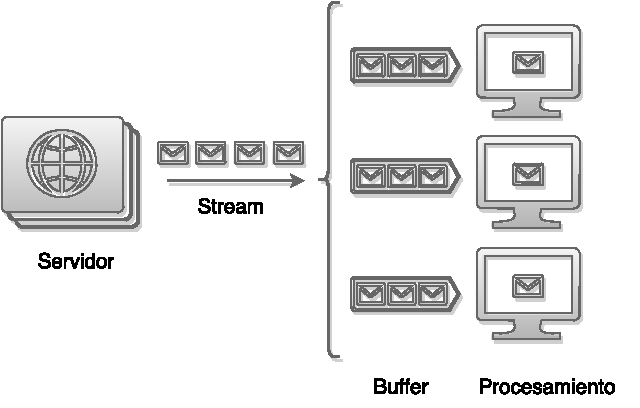
\includegraphics[scale=0.7]{images/Streaming.pdf}
  \caption{Flujo de datos entre el servidor y los clientes.}
  \label{fig:streaming}
\end{figure}

Este tipo de técnica es útil cuando se desea procesar información en tiempo real, siendo relevante la temporalidad de los datos, como la reproducción \textit{online} de material multimedia. Los datos emanados por el \textit{streaming} pueden ser utilizados para el análisis y procesamiento de un SPS (Sistema de Procesamiento de \textit{Stream}). Un ejemplo de esto, es la \textit{Streaming API} proporcionada por Twitter, donde esta información se puede utilizar para estudiar los \textit{tweets}, los \textit{trending topic} o los \textit{hashtag} más utilizados para casos específicos, como campañas electorales o desastres naturales.

\section{Stream processing}
\label{sec:streamProcessing}

\textit{Stream processing} es un paradigma de programación, el cual está orientado al procesamiento de un flujo de datos en tiempo real. Se centra en la programación de aplicaciones que puedan procesar la información en el momento, utilizando los recursos del sistema de forma paralela o distribuida para cumplir su objetivo, de tal manera que su procesamiento sea lo más cercano al tiempo real \citep{ChakravarthyJ09}.

Dentro de las aplicaciones existentes en el procesamiento de \textit{stream}, están el monitoreo de signos vitales, detección de fraudes, reproducción de videos \textit{online}. Para el funcionamiento correcto de estas aplicaciones, es necesario cumplir con ciertas características. Es por esto que se han propuesto ciertos requerimientos para el procesamiento continuo de datos \citep{andrade2014fundamentals}, los cuales son desglosados a continuación:

\begin{itemize}
	\item \textbf{Procesamiento de grandes cantidades de datos}: esto significa que al tratar de procesar los datos, no se puede guardar en una base de datos y luego procesarlos, como en general lo realizan los sistemas de \textit{bash processing}. Por lo tanto es necesario otro mecanismo que pueda procesarlos mientras va llegando la información entrante. Por lo que al utilizar \textit{stream processing} soluciona este problema, dado que la información entrante es procesada a medida que van llegando los datos.
	\item \textbf{Limitaciones de ancho de banda y latencia}: se refiere a la comunicación que existe por parte del proveedor de datos, de tal manera que no sea una limitante en el procesamiento de los datos el ancho de banda o la latencia existente. Esto es importante, dado que no sirve un sistema de estimación de la bolsa del mercado con una latencia considerable, de tal manera que envíe datos obsoletos. Siempre se debe mantener una baja latencia, para poseer los datos lo más cercano al tiempo real.
	\item \textbf{Procesamiento de datos heterogéneos}: en su mayoría, los datos poseen distintos formatos, contenidos y niveles de ruido, por lo que es necesario realizar una normalización de estos, de tal manera de estandarizar el procesamiento.
	\item \textbf{Proporcionar alta disponibilidad a largo plazo}: es importante poseer un constante flujo de información, que sea estable y persistente en el tiempo, de tal manera que esté procesando constantemente los datos para el propósito designado. Si analizamos el funcionamiento de los sistemas, estos poseen un porcentaje de fallas, y los SPS no son la excepción, por ello es importante contar con un mecanismo de tolerancia a fallos que permita reducir la pérdida de información. De no existir, se puede perder información, comprometiendo la precisión de los resultados y requiriendo de un mayor tiempo para recolectar la información perdida o alcanzar un estado similar.
\end{itemize}

\section{Sistemas de procesamiento de stream}
\label{sec:SPS}

Entre los diferentes motores de procesamiento de datos masivos, existen los sistemas de procesamiento de \textsl{stream}, los cuales reciben grandes cantidades de datos que deben procesar de forma distribuida y en tiempo real, de ahora en adelante hablaremos de procesamiento \textsl{online} para hacer referencia al tiempo real. Para realizar esto, se requiere un cambio en el paradigma tradicional de \textsl{bash processing}, el cual almacena los datos, los que posteriormente son procesados de forma \textsl{offline} \citep{HawwashN14}. Este cambio implica el análisis sin almacenar los datos, por lo que estos fluyen mientras son procesados.

El paradigma utilizado se basa en grafos de procesamiento como muestra la Figura \ref{fig:grafo}, donde los operadores corresponden a las vértices del grafo, como por ejemplo analizadores de sentimientos, filtros de palabras o algún algoritmo en particular, y las aristas corresponden a los flujos de datos entre un operador y otro \citep{Shahrivari14}. Además de esto, los datos proporcionados son originados por un ente externo, ya sea \textit{streaming} de redes sociales, estadísticas del monitoreo de un sistema, o transacciones en la bolsa de comercio, la cual entrega los datos iniciales a los primeros operadores del grafo \citep{AppelFFB12}.

\begin{figure}[ht!]
  \centering
    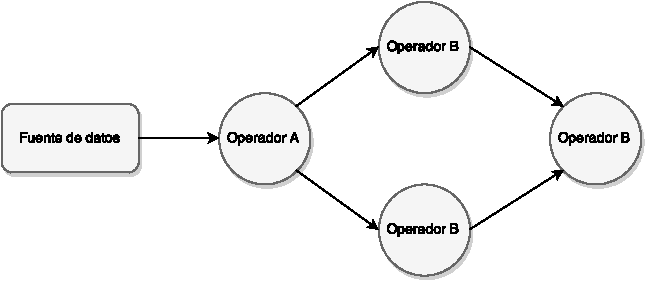
\includegraphics[scale=1]{images/SPS.pdf}
  \caption{Ejemplo de modelo de SPS.}
  \label{fig:grafo}
\end{figure}

Cabe destacar que los SPS son distribuidos, es decir, cada uno de los vértices del grafo son alojados en un nodo físico disponible en el ambiente en que se aloja el sistema, ya sea un \textit{cluster}, un \textit{grid} o un \textit{cloud}. Para lograr la comunicación entre los operadores, se utilizan sistemas anexos especialmente diseñados para este tipo de tareas, como Apache ZooKeeper \citep{HuntKJR10}. Este sistema es un servicio centralizado que mantiene la información de configuración y sincronización de las aplicaciones distribuidas que se posean. Por lo tanto, cada nodo al registrarse al servidor central, éste se encarga de señalar los nodos disponibles para la interacción entre ellos.

Las principales aplicaciones que se le dan a estos SPS, están orientadas al manejo de grandes cantidades de datos, las cuales deben ser procesadas para obtener información o estadísticas, como es el caso de detección de fraudes, recolección de información en caso de desastres o análisis de la interacción en las redes sociales. Para efectuar un procesamiento en tiempo real de los datos, \citep{StonebrakerCZ05} establece los siguientes requerimientos:

\begin{itemize}
	\item \textbf{Baja latencia}: este concepto está asociado con la comunicación fluida entre los distintos nodos del sistema, de tal manera que no existan altos \textit{delay} o retrasos en el procesamiento.
	\item \textbf{Consultas SQL}: poder realizar consultas a una base de datos, sin perder las propiedades del SPS, como el procesamiento distribuido. Para esto, se debe realizar un cambio en la forma de ejecutar las consultas, debido que no sólo es necesario realizar la consulta, sino también que se puedan unir las respuestas entregadas de forma paralela. Dado lo anterior, se hace necesario diseñar un sistema que cumpla con operadores adicionales a los utilizados en las consultas tradicionales por sistemas centralizados.
	%\item \textbf{Manejo de fallas en el flujo de dato}: es importante poseer sistemas que no se preocupen de la pérdida en los datos, debido que se posee como premisa que se van a perder datos en el procesamiento de estos, ya sea por las colas, \textit{delays} u otro problema asociado al procesamiento o la fuente de datos. Por lo tanto, al modelar la aplicación no es necesario lidiar con este tipo de fallas.
	\item \textbf{Generar resultados predecibles}: cuando se realizan consultas en el sistema, existe la posibilidad que sean correctas sólo por un período de tiempo, debido a alguna falla en el sistema que genere una pérdida en el estado del operador. Por lo tanto, es necesario garantizar que el resultado sea determinístico y persistente en el tiempo, ya sea respaldando la información u otro mecanismo, de tal manera que si se realiza una consulta, el resultado sea consistente u homólogo con el transcurso del tiempo.
	\item \textbf{Integrar almacenamiento y flujo de datos}: en general, cuando se trabaja con procesamiento de datos, es importante guardar estados en el sistema, de tal manera que los datos entrantes vayan verificando, modificando o eliminado la información que se posea. En un operador que cuente palabras, es necesario soportar variables que guarden las estadísticas de la información entrante. Otro tema importante es la uniformidad de los datos, como se había explicado anteriormente, en general se trabaja con datos heterogéneos, por lo que se requiere estandarizarlos para su procesamiento, de tal manera que no exista una discordancia en la información procesada.
	\item \textbf{Garantizar la seguridad y disponibilidad de los datos}: este requerimiento está orientado en poseer mecanismos de \textit{checkpoint}, técnica utilizada para respaldar el estado del operador cada cierto período de tiempo, y tolerancia a fallas. Por lo que en caso de existir alguna falla, el sistema pueda volver a estar disponible y sin perder una cantidad considerable de información, ya sea en las estadísticas o estados del sistema.
	\item \textbf{Partición y escalabilidad automática de las aplicaciones}: es importante también distribuir la carga entre los distintos procesadores o máquinas, deseando idealmente una escalabilidad incremental. Esto significa que el flujo de datos sea entregado a los distintos recursos que se poseen, y en caso de necesitar más recursos incrementarlos \citep{bookTanenbaum}. Si bien no sucede siempre, se espera que esto sea automático y transparente.
	\item \textbf{Procesamiento y respuesta instantánea}: cuando se plantea el uso de los SPS, se apuesta por un sistema que entregue respuestas en un tiempo lo más cercano al real. Este requerimiento hace necesario lidiar posibles sobrecargas de los operadores, las cuales afectan al rendimiento del sistema. Por lo tanto, se hace necesario abordar estos posibles escenarios proveyendo una solución de bajo \textit{overhead}, esto quiere decir con bajo costo de implementación o recursos necesarios para su funcionamiento, aumentando así la eficiencia y el rendimiento del sistema.
\end{itemize}

Cada sistema de procesamiento de \textsl{streaming} está basado en un modelo de procesamiento en particular. Por ejemplo, S4 utiliza el modelo de procesamiento \textsl{push} \citep{s4yahoo}, y Storm el modelo \textsl{pull} \citep{stormtwitter}.

El primer modelo llamado \textit{push}, consiste en el envío de datos desde el operador. La ventaja de este modelo empleado por S4 radica en la abstracción en el envío de datos, sin embargo no asegura el procesamiento de estos, debido a que no existe un mensaje de respuesta al ser entregado al operador. En la Figura \ref{fig:sps-push} se puede ver el Operador A como envía los datos al Operador B, donde en caso que el Operador B esté procesando un dato, éste lo guarda en cola. Debido a la forma en como se realiza el envío del evento, éste no asegura que llegue efectivamente, en caso que suceda una falla en la comunicación, habiendo una abstracción en el envío de los eventos por parte del operador emisor.

\begin{figure}[ht!]
  \centering
    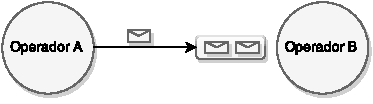
\includegraphics[scale=1]{images/SPS-Push.pdf}
  \caption{Modelo push de procesamiento.}
  \label{fig:sps-push}
\end{figure}

Por otra parte, el segundo modelo llamado \textit{pull}, se basa en la petición de datos a un operador, por lo que son enviados solo si son requeridos. Si bien este modelo asegura procesamiento de los datos, genera una menor abstracción al programador, dado que en el primer modelo sólo se indica a que operador deben ir los datos, en cambio en el segundo se debe indicar quién lo envía y quién lo recibe. En la Figura \ref{fig:sps-pull} (a) se observa que existen dos operadores, donde se solicita por parte del Operador B el envío de un dato para ser procesado, para que posteriormente en la Figura \ref{fig:sps-pull} (b) el Operador A envía el dato para que posteriormente sea procesado por el Operador B.

\begin{figure}[ht!]
  \centering
    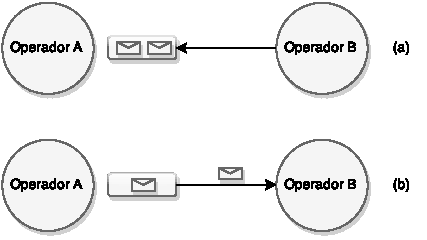
\includegraphics[scale=1]{images/SPS-Pull.pdf}
  \caption{Modelo pull de procesamiento.}
  \label{fig:sps-pull}
\end{figure}

\subsection{S4}
S4 (Simple Scalable Streaming System) \citep{s4yahoo} es un sistema de propósito general, distribuido y escalable que permite diseñar aplicaciones pueden procesar flujos de datos de forma continua y sin restricciones. S4 está inspirado en MapReduce \citep{2010Lin}, y está diseñado en el contexto de minería de datos y algoritmos de aprendizaje de máquina en Yahoo! Labs para sistemas de publicidad \textsl{online}. Cada evento en S4 es descrito como un par (clave, atributo), cuyos pares pueden ir agregándose a medida que sea necesario. La unidad básica son los elementos de procesamiento (PEs, por sus siglas en inglés). Los PEs pueden emitir o pueden publicar resultados y son alojados en servidores llamados nodos de procesamiento, llamados PNs. Los PNs son responsables de escuchar eventos, rutear eventos a los PEs del nodo y despachar eventos a través de la capa de comunicación. Los eventos son encaminados usando una función de \textsl{hashing} sobre los valores de los atributos hacia el PE apropiado. Para este fin, en la capa de comunicación utiliza Apache ZooKeeper \citep{HuntKJR10}, el cual provee manejo de \textit{clusters} y reemplazo automático de nodos que fallan. S4 usa encaminamiento estático, es parcialmente tolerante a fallas, y no posee mecanismos de balanceo dinámico de carga.

\subsection{Storm}
Storm \citep{bookstorm} es una plataforma similar a S4, orientada a la computación de flujos de datos en tiempo real de forma escalable. El modelo de programación está basado en dos primitivas básicas para la transformación de flujos de datos que deben ser implementados de acuerdo a la lógica de las aplicaciones: \textit{Spouts} y \textit{Bolts}. Un \textit{Spout} es una fuente de flujo de datos y un \textit{Bolt} hace una transformación de un solo paso sobre el flujo de datos, creando un nuevo flujo basado en la entrada que recibe. Transformaciones complejas requieren múltiples \textit{Bolts}, los cuales crean topologías o grafos, el nivel más alto de abstracción en Storm. La plataforma soporta tolerancia a fallas a través de un proceso maestro llamado Nimbus \citep{MiaoYJ14}, el cual garantiza el procesamiento de todos los mensajes a través del uso de una base de datos para su almacenamiento. Sin embargo, esta base de datos es su mayor desventaja respecto de S4 puesto que no es completamente distribuida. Storm define diferentes técnicas para el particionamiento de \textit{streams} de datos y para la paralelización de \textit{Bolts}, por lo tanto la asignación de máquinas para alguna actividad debe efectuarse de forma manual, lo que complica el desarrollo de aplicaciones. Al igual que S4, Storm usa Apache ZooKeeper \citep{HuntKJR10} en la capa de comunicación.

\section{Elasticidad}
\label{sec:elasticidad}

La propiedad de elasticidad en el área de \textit{Cloud Computing} o \textit{SPS}, está relacionado con la capacidad que el sistema tiene de adaptarse dinámicamente a las condiciones variables del sistema, como por ejemplo el tráfico. Esto quiere decir que aumente o disminuya los recursos que se utilicen, para que funcione de manera eficiente.

En el caso de \textit{Cloud Computing} existen estudios que han trabajado con esta propiedad como \citep{GongGW10, NguyenSGSW13, LehrigEB15}, donde el sistema se comporta de forma elástica, determinando dinámicamente la cantidad de máquinas virtuales necesarias en el sistema. Por otra parte, en los SPS, existen trabajos como \citep{GedikSHW14, IshiiS11, SchneiderAGBW09, MadsenTZ14, GulisanoJPSV12}, en que el sistema de forma dinámica determina la cantidad de operadores necesarios para realizar una tarea en específico, como se ve representando en la Figura \ref{fig:elasticidad}, donde la cantidad de operadores B cambia dinámicamente según el rendimiento del sistema.

\begin{figure}[!ht]
	\centering
	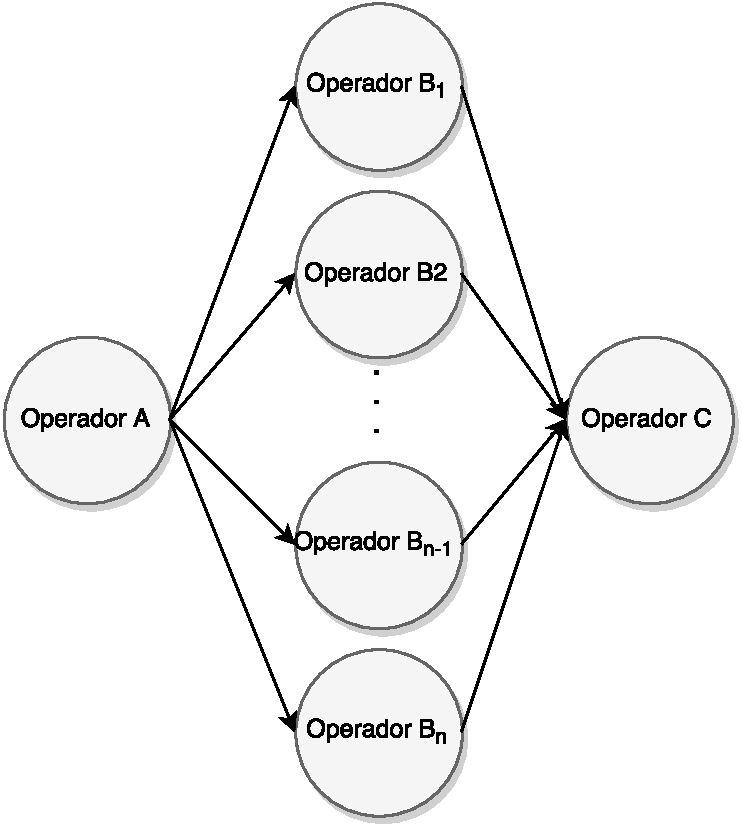
\includegraphics[scale=0.55]{images/Elasticidad.pdf}
	\caption{Elasticidad en un SPS.}
	\label{fig:elasticidad}
\end{figure}

Un ejemplo práctico de elasticidad es el supermercado, donde se debe considerar la cantidad de cajas necesarias para atender de manera eficiente los $n$ clientes que van llegando en un período de tiempo. Si se estudia el período de la mañana, en general, se tiene un bajo flujo de personas que acude al supermercado, en comparación con la tarde, pero alto comparado la medianoche. Por lo tanto, en los horarios de la tarde es necesario poseer una mayor cantidad de cajas disponibles que en la mañana, disminuyendo la cantidad nuevamente cuando el horario bordea la medianoche, adaptándose de forma elástica la cantidad de cajas disponibles en el supermercado.

En el trabajo realizado, se propone un sistema elástico dada la demanda de los distintos operadores. De esta manera, según el tráfico existente aumentan o disminuyen los operadores, de tal manera que trabaje de manera dinámica y de forma óptima.

\section{Procesos estocásticos}
\label{sec:procesosEstocasticos}

Se define proceso estocástico como una colección de variables aleatorias {$X_t$, con $t ~ \epsilon ~ T$}, las cuales están determinadas por algún comportamiento en el tiempo $t$. Esto significa que cada variable está tratada de forma discreta en el tiempo, sin poseer un proceso determinístico entre sus variables, es decir, que las variables dependan de la historia \citep{taylor2014introduction}.

Por lo tanto, se puede definir un estado como el posible comportamiento que puede tener una variable aleatoria en el sistema. Un ejemplo de esto es un modelo que contemple tres estados: estable, inestable y ocioso, y según el valor de la variable aleatoria, vaya cambiando de un estado a otro. Un caso de estudio utilizando el concepto de estados son las cadenas de Markov, las cuales consideran distintos estados, donde cada uno representa un comportamiento del sistema \citep{de1978calculus}.

Como se mencionó anteriormente, las cadenas de Markov son procesos estocásticos, las cuales se utilizan para soportar la predicción de carga en el modelo propuesto \citep{GongGW10}. De esta manera, se definen estados que son independientes en el transcurso del tiempo. Esto fue pensando con el fin de realizar análisis a futuro, tomando en consideración los datos \textit{a priori}.

\subsection{Cadena de Markov}
\label{subsec:cadenaMarkov}

Sea $X_t$ el valor de una variable aleatoria $X$ en un tiempo $t$, donde el conjunto de todos los valores posibles para $X$ se llama espacio de estado \citep{ching2006markov}. La variable aleatoria es un proceso de Markov si las probabilidades de transición entre dos estados cualquiera de $\Omega$ (definido como el universo de posibles estados), sólo depende del estado actual, como se denota en la Ecuación \ref{eq:defMarkov} y gráficamente en la Figura \ref{fig:procesoMarkov}. Cabe destacar que este tipo de proceso es un caso específico de los procesos estocásticos.

\begin{equation} \label{eq:defMarkov} 
	P_r(X_{t+r} = S_j | X_0 = S_k ; X_1 = S_l ; ... ; X_t = S_i) = P_r(X_{t+1} = S_j | X_t = S_i)
\end{equation}

\begin{figure}[ht!]
  \centering
    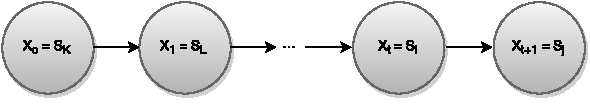
\includegraphics[scale=0.6]{images/ProcesoMarkov.pdf}
  \caption{Proceso de Markov.}
  \label{fig:procesoMarkov}
\end{figure}

Una cadena de Markov es una secuencia de variables aleatorias generadas por un proceso de Markov, como se denota en la Ecuación \ref{eq:cadenaMarkov}.

\begin{equation} \label{eq:cadenaMarkov}
	(X_0, X_1, X_2, ..., X_{n-1}, X_{n})
\end{equation}

La Ecuación \ref{eq:transicionMarkov} se define por sus probabilidades de transición. En la Figura \ref{fig:cadenaMarkov} se muestra un ejemplo de la transición del estado $i$ al estado $j$, dada la probabilidad $P_{ij}$.

\begin{equation} \label{eq:transicionMarkov}
	P_{ij} = P_r(i \rightarrow j) = P_r(X_{t+1} = S_j | X_t = S_i)
\end{equation}

\begin{figure}[ht!]
  \centering
    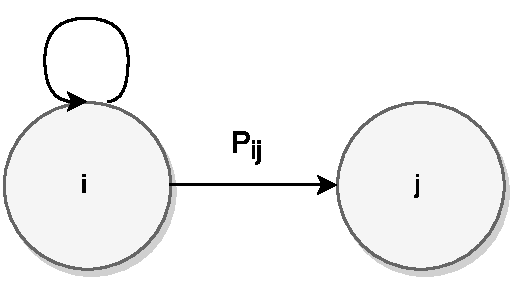
\includegraphics[scale=0.6]{images/CadenaMarkov.pdf}
  \caption{Cadena de Markov.}
  \label{fig:cadenaMarkov}
\end{figure}

En la Ecuación \ref{eq:matrizTransicion} se presenta una matriz de transición de finitos estados, donde la probabilidad de pasar de un estado a otro está determinado por una posición de la matriz, tomando en consideración que la suma de todas las transiciones de un estado debe ser igual a 1.

\begin{equation} \label{eq:matrizTransicion}
	P =
	\begin{bmatrix}
		P_{1,1} & P_{1,2} & \cdots & P_{1,n} \\
		P_{2,1} & P_{2,2} & \cdots & P_{2,n} \\
		\vdots  & \vdots  & \ddots & \vdots  \\
		P_{n,1} & P_{n,2} & \cdots & P_{n,n} \\
	\end{bmatrix}
	\hspace*{1cm} \sum_{j=1}^{n} P_{ij} = 1 ; \forall i
\end{equation}

En la Figura \ref{fig:ejCadenaMarkov} se muestra un ejemplo de una cadena de Markov simple, donde se analiza la probabilidad del clima de mañana dado el clima de hoy día. Como se puede observar, no se considera la historia del clima en la semana, sólo el del caso actual, lo cual es definido en los procesos estocásticos. Dada las probabilidades que transite de un clima a otro, se puede ver en la Ecuación \ref{eq:ejCadenaMarkov} la matriz de transición resultante.

\begin{figure}[ht!]
	\centering
	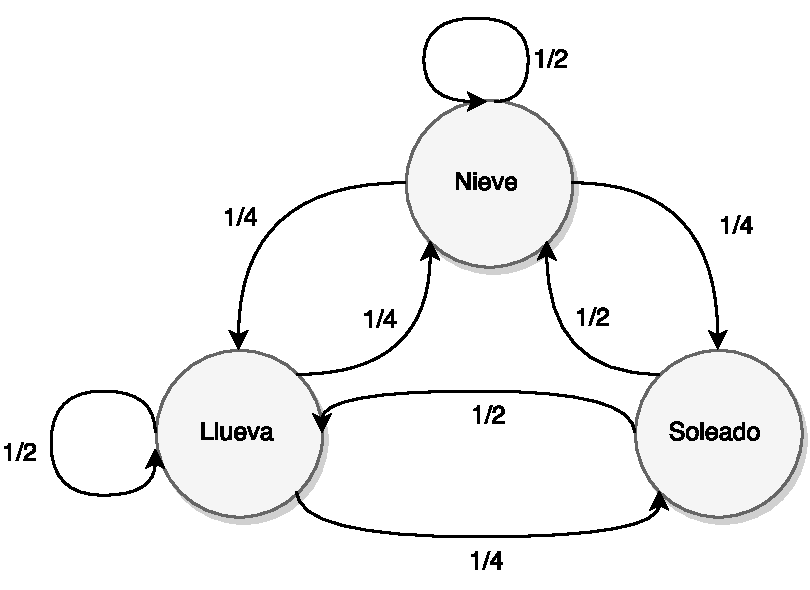
\includegraphics[scale=0.5]{images/EjCadenaMarkov.pdf}
	\caption{Ejemplo de cadena de Markov.}
	\label{fig:ejCadenaMarkov}
\end{figure}

\begin{equation} \label{eq:ejCadenaMarkov}
	P =
	\begin{bmatrix}
		\frac{1}{2} & \frac{1}{4} & \frac{1}{4} \\
		\frac{1}{2} & 0 & \frac{1}{2} \\
		\frac{1}{4} & \frac{1}{4} & \frac{1}{2}
	\end{bmatrix}	
\end{equation}

Si se desea saber la probabilidad que la cadena esté en el estado $S_i$ en el tiempo $t+1$, está dada por la ecuación de Chapman-Kolmogórov \citep{Papoulis1984}:

\begin{equation} \label{eq:chapman-kolmogorov1}
\begin{split}
	\Pi_{i} (t+1) &= P_r(X_{t+i}=S_i) \\
				  &= \sum _{k} P_r(X_{t+i} = S_i / X_t = S_k)·P_r(X_t = S_k)\\
				  &= \sum _{k} P_r(X_{t+i} = S_i / X_t = S_k)·\Pi_{k} (t)
\end{split}	
\end{equation}

En notación matricial:

\begin{equation} \label{eq:chapman-kolgorov2}
\begin{split}
	\Pi_{(t+1)} &= \Pi_{(t)}P\\
	\begin{bmatrix}
		\Pi_1 & \Pi_2 & \Pi_3
	\end{bmatrix} _{(t+1)}
	&= \begin{bmatrix}
		\Pi_1 & \Pi_2 & \Pi_3
	\end{bmatrix} _{(t)}
	\begin{bmatrix}
		P_{1,1} & P_{1,2} & \cdots & P_{1,n} \\
		P_{2,1} & P_{2,2} & \cdots & P_{2,n} \\
		\vdots  & \vdots  & \ddots & \vdots  \\
		P_{n,1} & P_{n,2} & \cdots & P_{n,n}
	\end{bmatrix}
\end{split}
\end{equation}

Usando recurrencia, se puede calcular la distribución estacionaria como se muestra la Ecuación \ref{eq:chapman-kolgorov3}, la cual indica el comportamiento a futuro de la cadena de Markov, dado los estados y transiciones que éste posee.

\begin{equation} \label{eq:chapman-kolgorov3}
\begin{split}
	\Pi (t) &= \Pi (t-1)P \\
				  &= \Pi (t-2)P^{2}\\
				  &= \Pi (0)P^{t} ; \Pi (0): \text{distribución inicial}
\end{split}
\end{equation}

\subsection{Trabajo relacionado}
\label{subSec:markovTrabajo}
Existen modelos predictivos que están basados en modelos matemáticos, los cuales simulan el comportamiento del sistema, ya sea del flujo o de la carga de un operador, de tal manera que pueden predecir cual es su estado en un tiempo futuro. En general, para poder realizar una predicción se analizan las variables en una ventana de tiempo, para posteriormente aplicar un modelo matemático que prediga la variación del sistema en la próxima ventana de tiempo que se tiene estipulada.

Dentro de las aplicaciones que se han realizado con modelos predictivos, se encuentra PRESS \citep{GongGW10}. En este sistema orientado a \textit{Cloud Computing} \citep{bookDistrSys}, analiza la cantidad de recursos disponibles, ya sea la memoria disponible o el uso promedio de CPU en las máquinas virtuales que se disponen en el \textit{Cloud}. Para realizar la predicción del estado del sistema, se aplica un modelo basado en cadenas de Markov, tomando sus estados como ventanas de tiempo en un determinado período. De esta manera, se analiza el estado del sistema en un tiempo en específico, para analizar si posee correlación con algún estado de la cadena de Markov, para posteriormente ver la transición de ese estado a otro y construir la matriz de transición. Posteriormente, con la ecuación de Chapman-Kolmogorov, se calcula la distribución estacionaria de la matriz de transición, de tal manera de saber en que estado está en la próxima ventana de tiempo, para finalmente analizar si es necesario algún cambio en el sistema.

Dentro de la misma línea de modelos predictivos, existe el sistema AGILE \citep{NguyenSGSW13} para \textit{Cloud Computing} que modifica las máquinas virtuales de forma elástica en un \textit{Cloud}. Lo que se realiza en este trabajo es aplicar la transformada de Fourier \citep{falk2012first} a series temporales, obtenidas mediante el muestreo de la carga de CPU en una ventana de tiempo. Luego, la función resultante se analiza con distintas frecuencias, de tal manera de solicitar la predicción de la próxima ventana de tiempo a cada una de las funciones creadas. De esta manera, se sintetizan todas predicciones realizadas por cada función para analizar el comportamiento del sistema en la próxima ventana de tiempo, y ver si es necesario aumentar o disminuir recursos de éste.

\section{Teoría de colas}
\label{sec:teoriaColas}

La teoría de colas se centra en el estudio matemático de las colas existentes en un sistema, cuyo caso de estudio es el desbordamiento de peticiones por parte del cliente al servidor \citep{queueingtheory}. En la Figura \ref{fig:teoriaColas} se muestra un ejemplo de un sistema basado en teoría de colas, donde existe $n$ productores que envían cierto flujo de datos a los $m$ servidores disponibles, y en caso de no estar disponibles, se genera una cola de espera en el sistema.

\begin{itemize}
	\item \textbf{Productor}: es quién provee la fuente de entrada para el servidor, de tal manera que procese según la necesidad que se posea.
	\item \textbf{Cola o línea de espera}: la cual está encargada de almacenar la información emanada por el productor en caso que los servidores estén ocupados, para que posteriormente sean procesados.
	\item \textbf{Servidor}: es quién procesa la información disponible en la cola, de tal manera de entregar una fuente de salida con los datos o información deseada.
\end{itemize}

\begin{figure}[!ht]
	\centering
	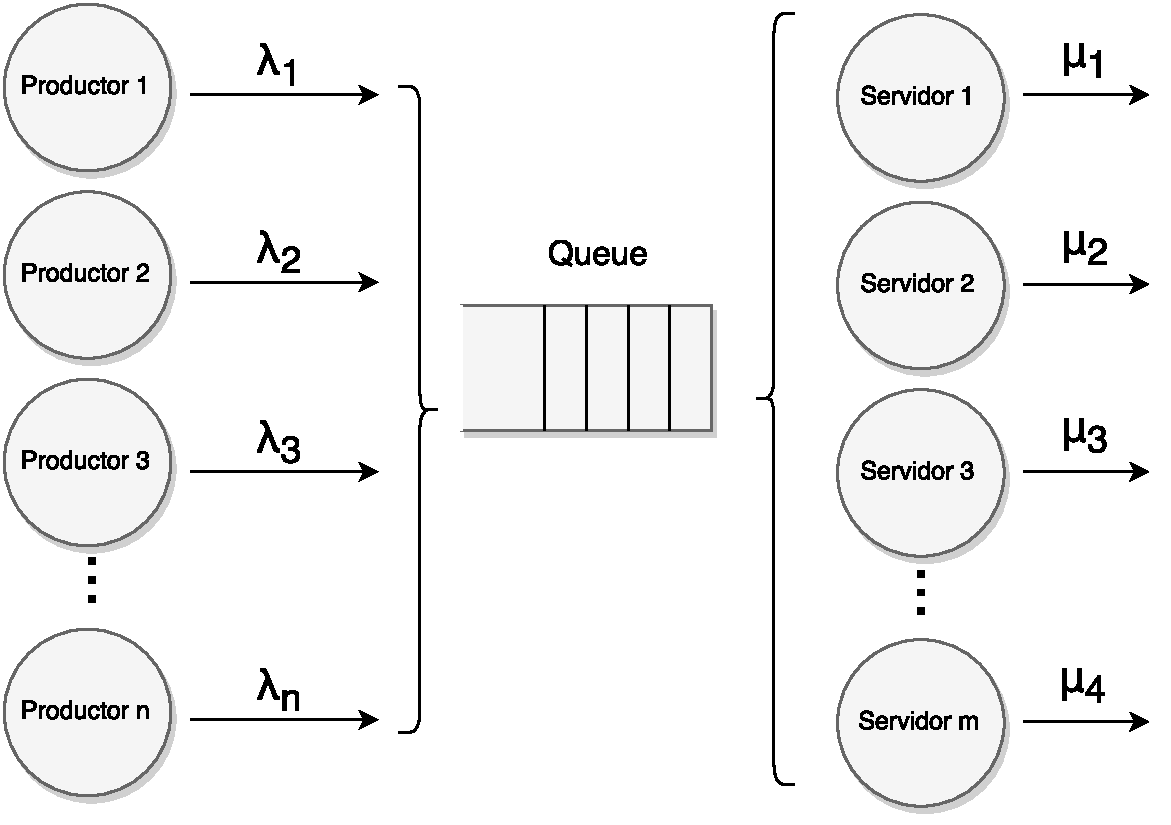
\includegraphics[scale=0.6]{images/TeoriaColas.pdf}
	\caption{Ejemplo de un sistema basado en teoría de colas.}
	\label{fig:teoriaColas}
\end{figure}

Además de esto, se tienen ciertos componentes importantes en el sistemas, definidos a continuación:
\begin{itemize}
	\item \textbf{Tasa de llegada}: denotado $\lambda$, es la cantidad de datos, eventos o información que van llegando en un determinado período de tiempo, la cual está determinada por los productores que existan en el sistema.
	\item \textbf{Tasa de procesamiento}: denotado $\mu$, también llamado tasa de servicio, es la cantidad de datos, eventos o información que salen del sistema, producto del procesamiento provisto por cada servidor.
	\item \textbf{Tasa de rendimiento}: denotado $\rho$, es el porcentaje de utilización del sistema, donde $\rho = \frac{\lambda}{s\mu}$, siendo $s$ la cantidad de servicios disponibles, definiendo así un sistema estable si es que $\rho < 1$, dado que la capacidad de procesamiento es mayor que la tasa de llegada.
	\item \textbf{Disciplina de la cola}: significa el método utilizado para extraer los datos encolados en el sistema, para esto puede aplicarse los métodos \textit{FIFO}, \textit{LIFO}, \textit{RSS}, entre otros.
\end{itemize}

Este tipo de modelos se puede aplicar a los SPS, debido que el operador emisor o la fuente de datos es el productor, y el operador receptor es el servidor del sistema. Por lo que existe un problema interesante a analizar debido a las posibles sobrecargas en los operadores. Por ejemplo, si se tiene un operador con una tasa de llegada $\lambda$ y una tasa de servicio $\mu$, donde $\mu < \lambda$, se tiene un sistema inestable, debido que se procesa más lento de lo que llegan los datos. Esto genera colas por lo que es necesario un aumento del rendimiento del sistema, debido que $\rho > 1 $, lo que significa que el sistema se encuentra inestable, generándose colas en éste. Es por esto, que para estabilizar el sistema, es necesario modificar la cantidad de réplicas existentes de ese operador del SPS, de tal manera de mejorar el rendimiento del sistema.
\chapter{Balance de carga en SPS}
\label{cap:estadoDelArte}

\section{Perspectivas de balance de carga}
\label{sec:perspectivasBC}
Dentro de la literatura se han encontrado distintas perspectivas al problema de balance de carga en un SPS, las cuales consideran los recursos físicos como fuente del problema de la sobrecarga del sistema, y otro enfoque que considera los recursos lógicos como el foco del problema.

\subsection{Recursos físicos}
\label{subsec:recFisicosBC}
En esta perspectiva se toma en consideración la sobrecarga del sistema dado las limitantes físicas que éste posea, ya sea por condiciones de los recursos disponibles o por el ambiente de desarrollo. Para esto, se consideran distintos parámetros como umbrales, los cuales si son sobrepasados debe aplicarse alguna estrategia para aliviar la carga del sistema. Estos umbrales pueden ser el nivel \textit{Service Level Objective} (SLO) \citep{sturm2000foundations}, porcentaje de CPU utilizada o disponibilidad de la memoria \citep{Dong06schedulingalgorithms}.

Una de las soluciones con la perspectiva anterior es lo propuesto en Borealis \citep{XingZH05}, donde considera la cantidad de carga de los nodos en ventanas de tiempo pre-determinadas, las cuales son manejadas por un coordinador centralizado. Este coordinador se encarga de analizar los recursos del sistema, y en caso que se sobrepase el umbral propuesto, se debe migrar los operadores que estén en ese nodo para luego ser enviados a otro nodo candidato con menor cantidad de carga. Esta estrategia no soluciona el problema de rendimiento del sistema, sino de la máquina, debido que sólo mueve el problema de una máquina a otra. Para elegir al nodo candidato, se realiza un análisis de correlación que existe entre el operador y el nodo candidato, de esta manera, no necesariamente va a ser enviado a otro nodo con menor carga, sino también el más cercano. Dentro de los problemas que pueden existir en este sistema radican en la conexión entre los distintos nodos, por lo que para las pruebas se considera un buen ancho de banda, de tal manera que aparente una red sin limitaciones de este tipo.

Otra de las soluciones que se han propuesto es lo realizado por Flood \citep{Alves2010flood}, la cual propone un DPS (\textit{Distributed data stream processing}) que considera ciertos factores físicos para agregar o eliminar máquinas virtuales en Amazon EC2 \citep{amazonec2}. Para esto, se posee un administrador que considera las estadísticas en tiempo de ejecución como la cantidad de CPU utilizada, latencia o memoria disponible, las cuales considera para ver en que rango está de los umbrales establecidos, y posteriormente agregar o eliminar recursos de manera elástica al sistema según un algoritmo reactivo implementando.

\subsection{Recursos lógicos}
\label{subsec:recLogicosBC}
%A diferencia de la física, aquí se consideran los componentes lógicos del sistema, como por ejemplo, una sobrecarga en algún operador. De esta manera, en las distintas soluciones se pueden encontrar soluciones en cuanto a la carga existente en el operador o la cantidad de cola que posea, de tal manera, que estos sean los umbrales a considerar para generar una mejora en el sistema.

A diferencia de la perspectiva de recursos físicos, en esta perspectiva lógica se consideran los componentes lógicos del sistema, es decir, el foco está en los operadores y su carga de trabajo. Las distintas soluciones que se presentan, analizan componentes como el flujo de datos o el tamaño de la cola de un operador, tomando esos parámetros y definiendo umbrales en los algoritmos implementados para realizar mejoras en el sistema.

% Enfoques de la perspectiva lógica

Dado esta perspectiva, se han presentando dos tipos de enfoques: el estático y el dinámico \citep{Gupta99loadsharing}. El primer enfoque está centrado en un modelo definido y fijo antes de la inicialización del sistema, sin considerar el estado del mismo. En cambio, el segundo enfoque está basado en un modelo que analiza el sistema según su estado en el transcurso de su ejecución.

%El primer enfoque se centra en la confección de un modelo definido y fijo antes de iniciar el sistema y que no varía en el tiempo. En cambio, el segundo se basa en la adaptación del sistema según su estado en tiempo de ejecución.

\subsection{Enfoque estático}
\label{subsec:enfoqueEstaticoBC}
Este enfoque se ha implementando en distintos sistemas de procesamiento de \textsl{stream}, donde no se depende del estado del sistema \citep{stormtwitter, s4}. De esta manera, no existe una interrupción en la ejecución o un cambio debido al estado del sistema \citep{CasavantK88}. Por lo tanto, no se considera variables como la carga o cola del operador, sólo se aplican técnicas que administren el flujo de los datos en el sistema.

%\textsl{Storm} utiliza la técnica de distribución de operadores según alguna política, tomando el enfoque estático \citep{stormtwitter}. El sistema configura el número de operadores que son necesarios para realizar una tarea, para que después estos sean repartidos en los distintos nodos disponibles según la política de \textit{Shuffle grouping}. Esta técnica basada en algoritmos de planificación \citep{bookScheduling}, consiste en distribuir los operadores en los distintos nodos utilizando una planificación \textsl{Round-Robin}, de tal manera que la cantidad de operadores sea uniforme en los nodos del sistema \citep{bookstorm}.

\textsl{Storm} utiliza distintas técnicas de distribución de las tuplas en los operadores según la política que se desee, todas tomando un enfoque estático \citep{stormtwitter}. Dentro de las políticas que existen están \textit{Shuffle grouping}, \textit{Fields grouping}, \textit{Partial Key grouping}, \textit{All grouping}, \textit{Global grouping}, \textit{None grouping}, \textit{Direct grouping} y \textit{Local grouping}.

La política de \textit{Shuffle grouping} se enfoca en distribuir las tuplas de forma homogéneas en los $n$ operadores que se encuentren en el grafo, utilizando la planificación \textit{Round-Robin} \citep{bookScheduling}, de esta manera la cantidad de tuplas se distribuye de forma homogénea en el sistema. Una de las principales fallas es que la tasa de procesamiento de las tuplas no siempre es la misma, por lo tanto puede existir una sobrecarga en un operador en particular, dado que éste recibe una mayor cantidad de tuplas que requieren un mayor tiempo de procesamiento. Otra de las políticas utilizada es \textit{Fields grouping}, la cual determina ciertas llaves a un operador determinado. Por ejemplo, se contiene un flujo de datos que se determinan por el identificador de los usuarios, de ser así, desde cierto rango de letras corresponden a cierto operador, de tal manera de dividir equitativamente según la cantidad de caracteres existentes. Si bien genera un determinismo en el procesamiento de las llaves, puede existir una sobrecarga de un operador en particular, debido a que una llave se repite con mayor frecuencia que otras, lo cual es demostrado en la ley de potencia \citep{rushton2010handbook}.

%Otra técnica es el uso de la función \textsl{hash} \citep{RogawayS04} para distribuir los operadores en el grafo, como lo planteado en S4 \citep{s4yahoo}. Esto consiste en aplicar lo anterior a algún atributo del evento, mapeando el evento al operador que corresponda de los $n$ operadores disponibles según el valor de la función. Cabe destacar que si no existe un operador mapeado con la imagen de la función, el sistema clona uno existente evaluando el nuevo con la imagen de la función como identificador. De esta manera, esta técnica provee dinamicidad respecto a la cantidad de operadores en el sistema.

Por otra parte, se encuentra el funcionamiento de S4, cuya política es similar a la de \textit{Fields grouping} de Storm, la diferencia es que un operador no le corresponde un conjunto de llaves, sino que posee una llave única. Esto quiere decir que cada llave se le asigna un operador, y en caso de no existir un operador para el valor de esa llave, se crea un nuevo operador de manera automática. Debido a la infinidad de combinaciones de llaves que pueden generarse, S4 recomienda aplicar una función \textit{consistent hashing} \citep{X11cp}. Esta técnica provee dinamismo en la cantidad de operadores en el sistema, pero al igual que la \textit{Fields grouping} puede sobrecargar un operador, debido que una llave posee mayor frecuencia que las otras, como se expresa en la ley de potencia, debido que un porcentaje de llaves es más usada que otras, como es el caso de las palabras utilizadas en el diccionario \citep{rushton2010handbook}.

Una ventaja del enfoque estático es el bajo costo de la implementación de los métodos, lo cual es beneficioso para sistemas con bajos recursos. Por otra parte, una desventaja existente es la existencia de puntos críticos en la topología, es decir, que un operador recibe más carga que sus pares, por lo que no se asegura que la cantidad de flujo sea repartido de forma homogénea. Si bien, no es una solución óptima, es un buen complemento para un modelo con el enfoque dinámico.

\subsection{Enfoque dinámico}
\label{subsec:enfoqueDinamicoBC}

%Este enfoque está basado en el estado del sistema, donde según las variables y estado de cada uno de sus atributos, genera una acción en el sistema \citep{CasavantK88}. Esto significa que si el sistema posee alguna anomalía, como una sobrecarga en un operador o latencia entre distintos nodos, se realiza un cambio en el sistema, con el fin de solucionar estos problemas. Para poder dar una solución al problema de sobrecarga, se pueden utilizar dos tipos de modelos: reactivo y predictivo.

Este enfoque está basado en el estado del sistema, siendo esto el parámetro base para optimizar su rendimiento \citep{CasavantK88}. Esto significa que si el sistema posee una una sobrecarga o alta latencia entre nodos, es necesario realizar un cambio en la lógica del sistema con el fin de solucionar el problema. En este contexto se consideran dos modelos: reactivo y predictivo.

\paragraph{Reactivo:} este modelo está basado en el análisis de carga en el sistema a través de un monitor \citep{GulisanoJPSV12}, el cual recibe periódicamente las variables de cada uno de los operadores, y en caso que sobrepase un umbral, se aplica una técnica para aumentar el rendimiento bajo una métrica dada. El umbral puede estar basado en el tiempo de procesamiento, el tamaño de la cola u otra variable del operador \citep{BhuvanagiriGKS06}. Por ejemplo, en el trabajo de \citep{SchneiderAGBW09} se considera el rendimiento de cada operador, por lo que en caso de existir congestión en un operador, se procede a replicarlo, de tal manera que exista un operador adicional que puede recibir un flujo de datos y realizar la misma operación que el operador sobrecargado en paralelo.

Si bien estas soluciones en su mayoría son eficientes y poseen buen rendimiento, uno de los principales problemas es que no analiza el comportamiento a futuro, debido que sólo analiza y resuelve la situación en el momento. Otro problema son los falsos positivos, debido que puede ser que en un momento exista un \textit{peak} de tráfico, pero esto era sólo un caso particular del instante, por lo que llevar a cabo la replicación del operador es un costo innecesario.

\paragraph{Predictivo:} este modelo está basado en modelos matemáticos que calculan o estiman el comportamiento a futuro del sistema, dada cierta información que se posee del sistema, como flujo entrante o carga de la CPU. Si bien no existen modelos predictivos para SPS, si los existen en otras áreas, como se presentó en la Sección \ref{subSec:markovTrabajo} con cadenas de Markov y análisis de series temporales en \textit{Cloud Computing}.

\section{Técnicas de balance de carga}
\label{sec:tecnicasBC}

Existen distintas técnicas de balance de carga que utilizan alguno de los dos modelos presentados anteriormente, las cuales están enfocados a mejorar el rendimiento del sistema en caso de existir una sobrecarga \citep{HirzelSSGG13}. Dentro de las técnicas existentes se encuentran la planificación determinista \citep{XuCTS14, DongTS07}, \textit{load shedding} \citep{SheuC09}, migración \citep{XingZH05} y fisión \citep{GulisanoJPSV12, IshiiS11, GedikSHW14, FernandezMKP13}, si bien existen más, sólo se trataron estas porque se consideran las más relevantes y que han sido trabajadas en la literatura relacionada al dominio del problema.

\subsection{Planificación determinista}
\label{sec:planificacionBC}
%La planificación determinista \citep{DongTS07} se centra en la planificación según los recursos y estados del sistema \textit{a priori} según alguna métrica \citep{XuCTS14}. Una métrica utilizada es la frecuencia de datos estimada en un nodo u operador \citep{Ganguly09}. Esta técnica se utiliza, por ejemplo, en \textit{StreamIt} \citep{ThiesKA02}. Una de las limitaciones es que si bien realiza una predicción determinista de la frecuencia, no necesariamente es correcta a futuro, por lo que no se puede predecir las tasas de tráfico en el transcurso del procesamiento, sino sólo estimarlas al comienzo de la ejecución del sistema.

La planificación determinista se centra en los conocimientos \textit{a priori} del sistema, esto significa que se consideran las variables del entorno que se poseen y respecto a esto se toma una decisión de como debe actuar el sistema. 

En el área de \textit{Stream processing} se han realizado diferentes análisis de la estimación de frecuencia de \textit{data stream} en el sistema. Para poder realizar esto, se han considerado modelos matemáticos, tomando ventanas de tiempo de la frecuencia predicha y la real, para posteriormente generar con los datos una función que represente la frecuencia estimada del operador, es decir, el tráfico esperado que llegará al operador en la ejecución del sistema \citep{Ganguly09}. Pero no sólo se han considerado modelos matemáticos, sino también algoritmos que determinan la frecuencia del sistema dado el flujo de datos que se podría recibir \citep{BhuvanagiriGKS06}.

En otras áreas como red de sensores, se utiliza esta técnica en el envío de estadísticas de dispositivos móviles, los cuales manejan información \textit{a priori} de donde están los sensores, de tal manera de determinar según la intensidad de la frecuencia, localización o clima, a dónde debe enviar la señal para que se recolecte la información correspondiente \citep{DongTS07}.

Una de las limitaciones de la técnica, es que si bien realiza una predicción determinista de la frecuencia, no necesariamente es correcta a futuro. Esto se debe a que puede analizarse respecto al promedio, pero pueden surgir \textit{peaks} o procesos inesperados del tráfico en el transcurso de la ejecución que pueden generar una sobrecarga en el sistema. Por lo tanto, la estimación al realizarse \textit{a priori}, sólo considera al inicio del sistema o ventanas de tiempo, por lo que puede existir un porcentaje de error considerable. Por otra parte, se considera que esta técnica posee mejor rendimiento si es que la frecuencia o función analizada es estacionaria, caso que raramente ocurre en el tráfico de internet o redes sociales, debido que suceden eventos externos que influyen en el tr\'afico analizado \citep{KarpSP03}.

% Darle una vuelta a esto...

%Es por esto, que no se considera una buena técnica para aplicar en los casos de estudio, debido que se desea trabajar con tráficos dinámicos, los cuales no poseen análisis estacionarios, sino 

\subsection{Load Shedding}
\label{sec:loadSheddingBC}
%Otra estrategia está orientada a descartar eventos de un operador sobrecargado, de tal manera de no generar colas en el sistema. Esta estrategia que si bien no está implementada en el sistema por defecto de S4, puede habilitarse \citep{s4}. Otro ejemplo, es la trasmisión de vídeo \textit{streaming}, donde se descartan los datos que son de baja calidad, para procesar en su mayoría información de alta calidad \citep{SheuC09}. Esta solución está pensada para disminuir la carga, perdiendo la exactitud de la información debido a la pérdida de datos. Por lo tanto existe una menor fiabilidad en el sistema en caso de realizar operaciones de transacción \citep{bookDistrSys}.

En los SPS también se utiliza la técnica de \textit{load shedding}, que consiste en descartar eventos del sistema en caso de existir una sobrecarga, ya sea un máximo en el tamaño de la cola, tasa de rendimiento u otro factor. En la Figura \ref{fig:loadShedding} se observa que existe un operador A, el cual recibe datos en un período de tiempo, debido a la cola que existe por parte del sistema, se considera utilizar un operador denominado \textit{Shedding}, que en caso de existir un flujo de datos mayor al umbral propuesto, va a descartar los eventos que excedan el umbral. Por ejemplo, en la transmisión de \textit{video streaming}, al enviar el flujo de información existe un administrador que está analizando el contenido a procesar, por lo que en caso de llegar datos de baja calidad, se descartados por éste. De esta manera, al existir menor cantidad de ruido, existe un mejor procesamiento del video, teniendo una mejor calidad en la visualización de los videos, dado que en su mayoría se procesan datos de alta calidad \citep{SheuC09}. 

\begin{figure}[!ht]
	\centering
	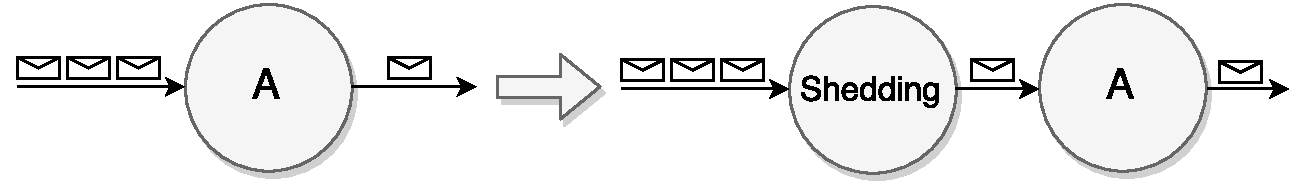
\includegraphics[scale=0.6]{images/LoadShedding.pdf}
	\caption{Load shedding en un SPS.}
	\label{fig:loadShedding}
\end{figure}

En el mundo de los SPS, varios poseen este tipo de estrategia, como por ejemplo S4 \citep{s4}, donde se establece una cota superior de eventos en cola, y en caso que su cola sea igual al límite establecido, los eventos entrantes serán descartados. Otro sistema que aplica esta técnica es Aurora \citep{aurora}, el cual se basa en procesamiento de datos por ventanas de tiempo, por lo que en caso de existir una ventana de tiempo con una mayor cantidad de eventos de lo estipulado, se descarta el exceso de eventos.

Si bien esta técnica es simple y de bajo costo, siendo pensada para la disminución rápida de carga, existe una baja en la precisión y fiabilidad del procesamiento de los datos. Por ejemplo, en el caso de la transferencia de video no es trascendental, dado que son pocos los pixeles perdidos, pero en una recopilación y análisis de estadísticas, esto da una menor precisión de la información obtenida por el sistema, dado que puede perderse información que indique comportamientos de los datos estudiados.

\subsection{Migración}
\label{sec:migracionBC}
%También se encuentra la migración, en el cual según el estado del sistema se migran los operadores de un nodo a otro. En \citep{XingZH05} se implementa   esta técnica, y si bien genera una menor carga en distintos nodos, produce un alto costo en la transferencia de los datos. Al realizar la transferencia de los datos, existe una menor tolerancia a fallos, a raíz de lo cual, se propone el uso de un búffer en el sistema, aumentando sus costos \citep{PittauACA07}.

La técnica de migración está basada en el traspaso de un operador de un nodo a otro, según el estado del sistema. En la Figura \ref{fig:migracion} se puede apreciar dos nodos, los cuales poseen tres y dos operadores respectivamente, pero debido a una sobrecarga del nodo 1, se realiza una migración de un operador al nodo 2, ya que este se encuentra con menor carga, de esta manera, se reparten homogéneamente la carga.

Si bien no existe una implementación que utilice la perspectiva según los recursos lógicos, si existe una que utiliza la perspectiva según los recursos físicos como es el caso de Borealis, el cual fue explicado anteriormente \citep{XingZH05}. Una de las principales críticas que se realiza a esta técnica, es que puede existir una falla en la comunicación del operador, donde no existe un mecanismo para evitar la pérdida de los datos. Debido a lo anterior, es que se propone el uso de \textit{buffer} que tengan respaldos de la información, aumentando los costos del sistema \citep{PittauACA07}.

\begin{figure}[!ht]
	\centering
	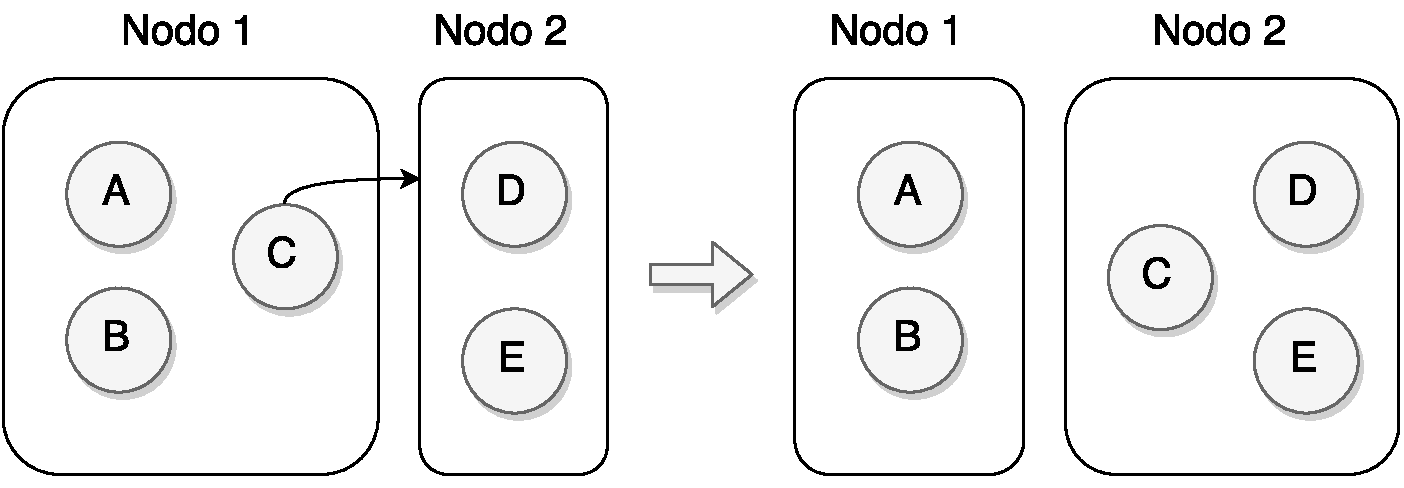
\includegraphics[scale=0.45]{images/Migracion.pdf}
	\caption{Técnica de migración en un SPS.}
	\label{fig:migracion}
\end{figure}

\subsection{Fisión}
\label{sec:fisionBC}

%Desde otra perspectiva, existen las técnicas de paralelización y replicación, las cuales se utilizan en caso de sobrepasar un umbral, el cual depende de la carga de un operador, nodo, entre otras variables. El primero consiste en paralelizar una tarea, la cual está determinada por un conjunto de operadores, en otro nodo físico \citep{IshiiS11}. En cambio, la replicación consiste en replicar un operador a nivel lógico del grafo \citep{MadsenTZ14}. Una de las características que existen en este tipo de soluciones es la elasticidad, que consiste en la capacidad de aumentar o disminuir la cantidad de operadores según la necesidad del sistema.

Otra técnica utilizada en el balance de carga es la fisión, o también llamada replicación, que permite paralelizar el procesamiento, la cual consiste en crear una réplica paralela del operador, sin perder el funcionamiento y estado, en caso de existir una sobrecarga en el operador. En Figura \ref{fig:fision} se presenta un operador A, el cual en primera instancia recibe un flujo de entrada $q_1$ y genera un flujo de salida $q_2$. Sin embargo, dado que este operador se sobrecarga se crean dos operadores extras, los cuales pasarán por una fase de \textit{Split} y posteriormente por una fase de \textit{Merge}. Estas fases son necesarias para distribuir y juntar la información respectivamente, y en general son de bajo costo, por lo que no es necesario replicar. En caso de ser necesario replicar el operador \textit{Merge}, debe existir un \textit{merge} de las distintas réplicas de éste, lo cual hace más complejo el diseño del sistema. En ciertos SPS se posee el planteamiento que el \textit{split} y el \textit{merge} son operadores que deben ser realizados por el programador, y no de forma automática por el sistema, como S4 o Storm. Una de las características que se posee de esta técnica es que permite generar un sistema elástico, donde se puede aumentar o disminuir la cantidad de operadores según los requerimientos del sistema.

\begin{figure}[!ht]
	\centering
	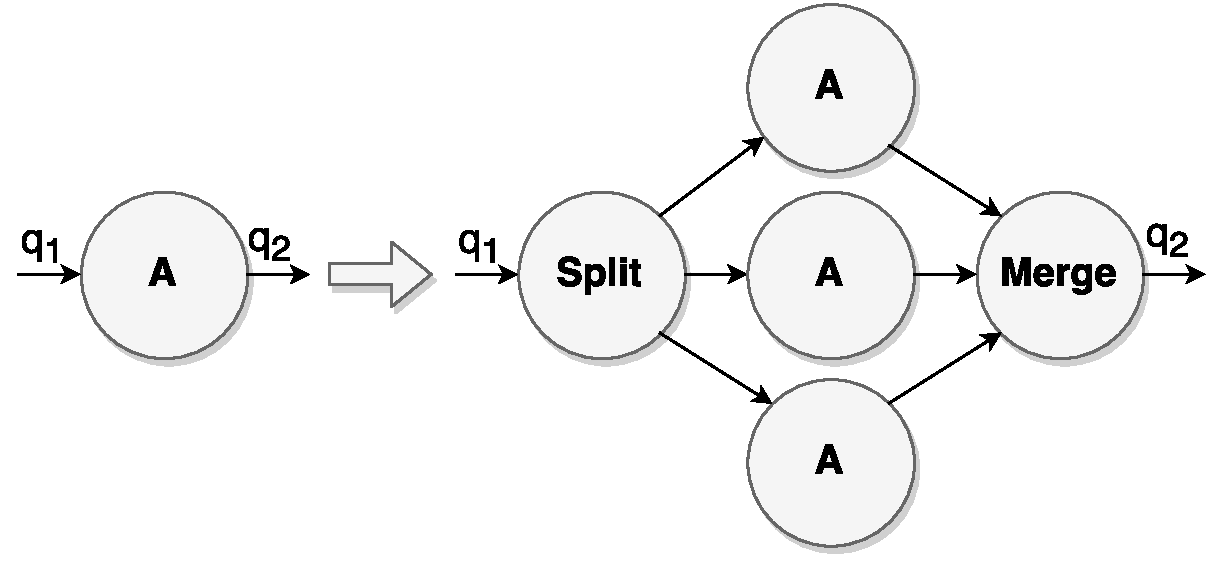
\includegraphics[scale=0.4]{images/Fision.pdf}
	\caption{Técnica de fisión en un SPS.}
	\label{fig:fision}
\end{figure}

%Una aplicación de la técnica de paralelización según el enfoque estático, es la paralelización de tareas de Storm \citep{stormtwitterdoc}, donde un conjunto de operadores realizan una tarea, indicado la cantidad de tareas que se desean ejecutar paralelamente en el sistema.

%Un ejemplo aplicado de esta técnica según el enfoque dińamico es StreamCloud \citep{GulisanoJPSV12}, que dada la cantidad de consultas que van llegando al sistema, se paralelizan las tareas existentes. Uno de los problemas que surge en estos casos son las operaciones con estado, como lo son los contadores o algoritmos de orden. La solución planteada es poseer un operador que realiza la tarea de \textit{merge}, que consiste en recibir las salidas de las tareas paralelas, agrupando los datos y proporcionando una salida según lo realizado por cada uno de las operaciones \citep{GedikSHW14}.

Una aplicación que utiliza la técnica de fisión bajo el enfoque estático, es la paralelización de tareas de Storm \citep{bookstorm}. Aquí se debe indicar en la topología del grafo la cantidad de operadores necesarios para realizar una tarea. De esta manera, por cada tarea se asigna un proceso, el cual tiene a su disposición $n$ hebras según la cantidad de operadores que se desea para cumplir dicha tarea.

Otro sistema que utiliza esta técnica, bajo un enfoque dinámico, es \textit{StreamCloud} \citep{GulisanoJPSV12}. Aquí según la cantidad de consultas realizadas al sistema se aumenta o disminuye la cantidad de operadores que cumplen las tareas que se solicitan. Para esto, es necesario un operador que distribuya los datos, denominado \textit{split}, y uno que junte la información entregadas por las réplicas del operador, denominado \textit{merge}. Por lo que este sistema sólo soporta ciertas operaciones, de tal manera que se creen de forma automática los operadores de \textit{split} y \textit{merge}. De esta manera, no existe problemas con los operadores con estado, como lo son los contadores y algoritmos de ordenamiento, dado que automáticamente realiza el procedimiento de separación y unión de los datos. Una de las características principales de este sistema, es aplicar el concepto de elasticidad, que aumenta y disminuye la cantidad de operadores según lo requerido por el sistema. Otros trabajos como \citep{GedikSHW14, SchneiderAGBW09} también aplican este método, y paralelizan las tareas de forma elástica, y con parámetros similares, sólo que su implementación es distinta, debido que este anterior propone utilizar \textit{Cloud} para el uso del SPS, en cambio los otros proponen el uso sobre \textit{clusters} de computadores. De esta manera, el enfoque se basa en la paralelización de las tareas entre las distintas máquinas, a diferencia del sistema utiliza \textit{Cloud}, donde aumenta o disminuye la cantidad de máquinas según la necesidad del sistema.

En \citep{FernandezMKP13}, aplican fisión en el caso que exista un cuello de botella en un operador. Para la detección de estas situaciones, se posee un monitor, el cual está consultando en un período de tiempo corto, el estado de cada uno de los operadores. De esta manera, en caso que un operador sobrepase el umbral de carga establecido, el cual está determinado por la utilización de CPU. En la Figura \ref{fig:ejFision} se puede ver un sistema, en el cual el operador \textit{u} está enviando un flujo de datos al operador \textit{o}. Una vez \textit{o} se sobrecarga (cuello de botella), este se debe replicar, hasta reducir la carga hasta un umbral deseado, en otras palabras, llegó a la cantidad de réplicas necesarios, y ya no es necesario replicar más.

\begin{figure}[!ht]
	\centering
	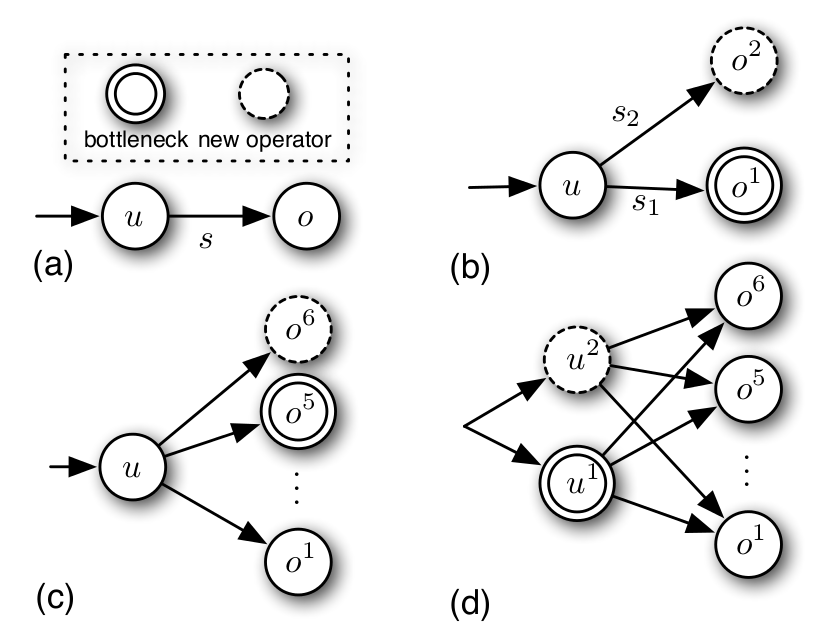
\includegraphics[scale=0.3]{images/EjFision.png}
	\caption{Ejemplo de replicación de los operadores \citep{FernandezMKP13}.}
	\label{fig:ejFision}
\end{figure}

Dentro de las desventajas existentes por parte de estos trabajos realizados, es que no utilizan la historia del operador para analizar el comportamiento a futuro de la carga. El uso de sistemas de predicción puede estabilizar el sistema cuando existen \textit{peaks} en el tráfico, debido que estos son detectados en el pasado, y se verifica si pueden ocurrir en el futuro, por lo que de ser así, se modifica el sistema en base a lo predicho.
\chapter{Dise\~no del sistema de distribución de carga}
\label{cap:disenoSistema}

Como se había mencionado en la subsección \ref{intro:problema}, el problema de la sobrecarga en un SPS está dado por la inflexibilidad existente en el grafo diseñado. Esto quiere decir, que en el momento que el sistema está funcionado, no existen un cambio en la cantidad de recursos necesarios, por lo que se vuelve ineficiente, debido a la sobrecargada en el sistema.

De ser así, es necesario un sistema que pueda proveer dinamismo en su estructura, así como también en el análisis de la carga tanto en el momento como a futuro, de tal manera que se complementen. Con estas condiciones, se diseñó un sistema de bajo costo que optimice su rendimiento, sin generar interrupciones en la ejecución del sistema.

\section{Análisis del sistema de distribución de carga}
Dentro del análisis realizado en la arquitectura del sistema implementando, se consideró una perspectiva en base a los recursos lógicos según el enfoque dinámico, definido en las subsección \ref{subsec:recLogicosBC} y \ref{subsec:enfoqueDinamicoBC} respectivamente, para el balance de carga de SPS. Esto debido que el trabajo presentando no analizó el comportamiento que tenga cada uno de los nodos del sistema, sino que se analizó el rendimiento que poseía cada uno de los operadores del grafo diseñado, siendo un problema de carácter lógico y no físico.

Respecto al estudio de las distintas técnicas implementadas, era necesario utilizar una que no tuvieran desventajas en cuanto a la pérdida de datos, inadaptabilidad con el tiempo y costo de implementación. Por lo tanto, se consideró que la mejor opción era utilizar la técnica de fisión, utilizando el mismo modelo de replicación que Fernández \citep{FernandezMKP13}, donde según una sobrecarga en el operador era necesario generar una réplica de ese operador. Dentro de las hipótesis planteadas, se pensaba que el costo de un operador iba a ser menor a la formación de las colas de datos en el sistema, lo cual podría variar según la arquitectura del SPS implementando.

En la Figura \ref{fig:ejReplicacion} se muestra un ejemplo de la replicación propuesta, donde en la parte (a) se presentan tres operadores, donde en uno de ellos (operador B) existe una sobrecarga, por lo que es necesario replicar el operador. En la parte (b) se realiza la replicación, pero todavía persiste la sobrecarga en el operador, por lo que se vuelve a realizar el mismo procedimiento, hasta que finalmente converge a la cantidad óptima de réplicas deseadas en el sistema en el período de tiempo analizado, como se muestra en la parte (c).

\begin{figure}[!hb]
	\centering
		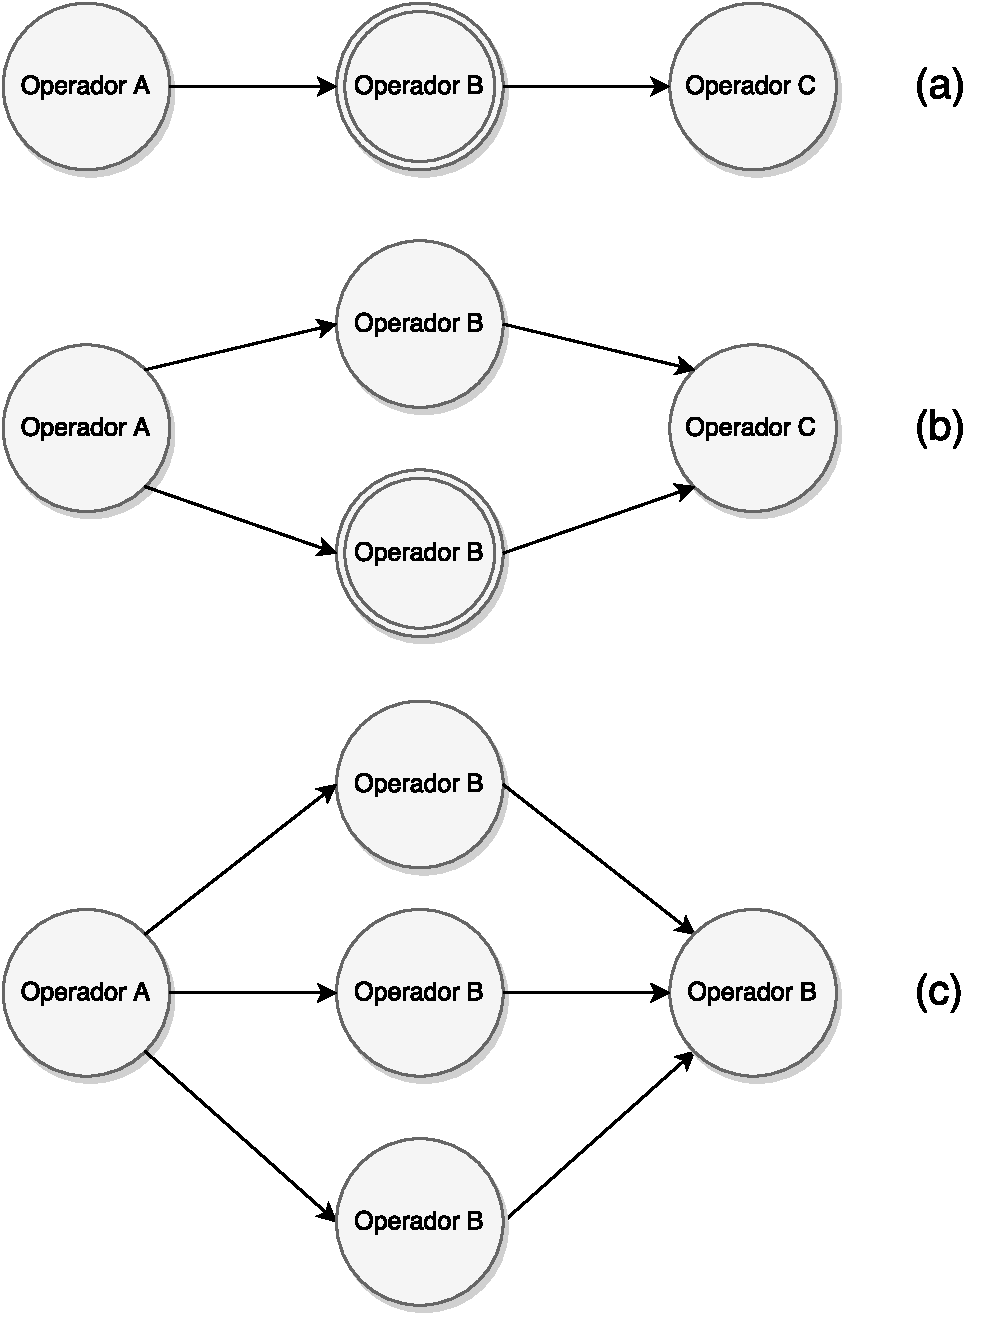
\includegraphics[scale=0.6]{images/EjReplicacion.pdf}
	\caption{Ejemplo de replicación del sistema propuesto.}
	\label{fig:ejReplicacion}
\end{figure}

%Para el diseño del sistema, era necesario contar con un umbral que determinara cuando el operador está o no sobrecargado, por lo que para esto se utilizaron conceptos de teoría de colas \citep{bose2013introduction}. Como los SPS están orientados en grafos, se posee tanto la tasa de llegada ($\lambda$) como la tasa de procesamiento ($\mu$) para cada uno de los operadores, como se ve representando en la Figura \ref{fig:analisisTeoriaColas}, donde la tasa de procesamiento de un operador es la misma tasa de llegada del siguiente operador en el grafo. Utilizando este tipo de conceptos, para cada operador se calculó la tasa de procesamiento ($\rho$), la cual esta definida por la tasa de llegada, la tasa de procesamiento y la cantidad de servicios disponibles en el sistema ($\rho = \frac{\lambda}{\mu \rho}$), cuyo valor nos indica el rendimiento del operador en cierta período de tiempo.

Para la detección de sobrecarga es necesario contar con un umbral que determine cuando está o no sobrecargado un operador, por lo que se utilizaron conceptos de teoría de colas \citep{bose2013introduction} para el análisis de esto. Como los SPS están orientados a grados, se puede obtener tanto la tasa de llegada ($\lambda$) como la tasa de servicio ($\mu$) de cada uno de los operadores, como se ve representando en la Figura \ref{fig:analisisTeoriaColas}, donde la tasa de procesamiento de un operador influye directamente en la tasa de llegada del siguiente operador en el grafo. Al utilizar estos conceptos, se cálculo la tasa de rendimiento ($\rho$), la cual está definida por la tasa de llegada, de procesamiento y la cantidad de réplicas del operador ($\rho = \frac{\lambda}{\mu \rho}$), cuyo valor representa el factor de utilización del sistema, donde se define un sistema estable si y sólo si $\rho < 1$.

\begin{figure}[!hb]
	\centering
		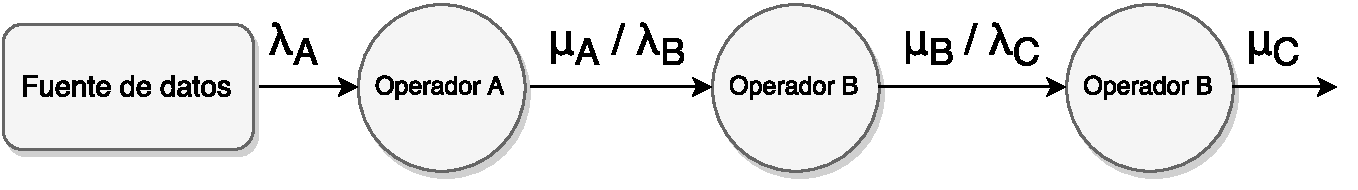
\includegraphics[scale=0.6]{images/AnalisisTeoriaColas.pdf}
	\caption{Enfoque de un SPS con conceptos de teoría de colas.}
	\label{fig:analisisTeoriaColas}
\end{figure}

Tomando en consideración el tipo de enfoque en el algoritmo de balance de carga y la elasticidad que se pretendía por parte del sistema, es que se trataron tres posibles estados en el sistema: ocioso, estable e inestable. El primer estado corresponde a un exceso en la cantidad de recursos necesarios. El segundo está definido por el rendimiento óptimo del sistema. Y por último, el tercero hace referencia a un sistema sobrecargado, donde es necesario mayor cantidad de recursos por parte de éste. Definido los posibles estados de cada operador, es que se tomó esto como base para el análisis y predicción de la carga en el sistema de distribución de carga.

Para el sistema propuesto, se consideraron dos tipos de algoritmos: predictivo, enfocado en el futuro y la historia del operador, y reactivo, analizando el comportamiento del momento. Esto fue diseñado con el fin de analizar dos factores, los \textit{peak} existentes en la historia del operador, dado el algoritmo predictivo, y otro que analice el comportamiento en el momento, haciendo uso del algoritmo reactivo, de tal manera de solucionar las anomalías que no son detectadas con la predicción.

Es importante denotar que dependiendo del tipo de caso es que un tipo de algoritmo va a funcionar mejor, por ejemplo si se posee una tasa de llegada dado una función exponencial, es necesario aumentar la cantidad de réplicas a medida que van aumentando la cantidad de réplicas en el sistema, por lo que en el predictivo podrá detectar este tipo de casos y aumentar la cantidad réplicas dado este patrón. Pero en el caso que no exista un patrón en la función, existe el algoritmo reactivo que analiza la situación en el momento para ver si es necesario o no cambiar la cantidad réplicas.

%Al diseñar un sistema que pudiera lidiar con dos tipos de algoritmos, era necesario considerar un algoritmo que pudiera administrar la cantidad de cargas, con tal utilizar el algoritmo necesario según el período existente en una ventana de tiempo, como también la cantidad de réplicas que deben aplicarse.

Como se diseñaron dos tipos de algoritmos que se complementaran, es necesario considerar un algoritmo que administre cual de los dos algoritmos se va a utilizar según el período analizado, como también la cantidad de réplicas que deben crearse o eliminar según el resultado del algoritmo utilizado.

Dado lo anterior, se diseño un sistema de distribución de carga con cuatro componentes: monitor de carga, analizador de carga, predictor de carga y administrador de réplicas, que se pueden apreciar en la Figura \ref{fig:componentesSistemas}.

\begin{figure}[ht!]
  \centering
    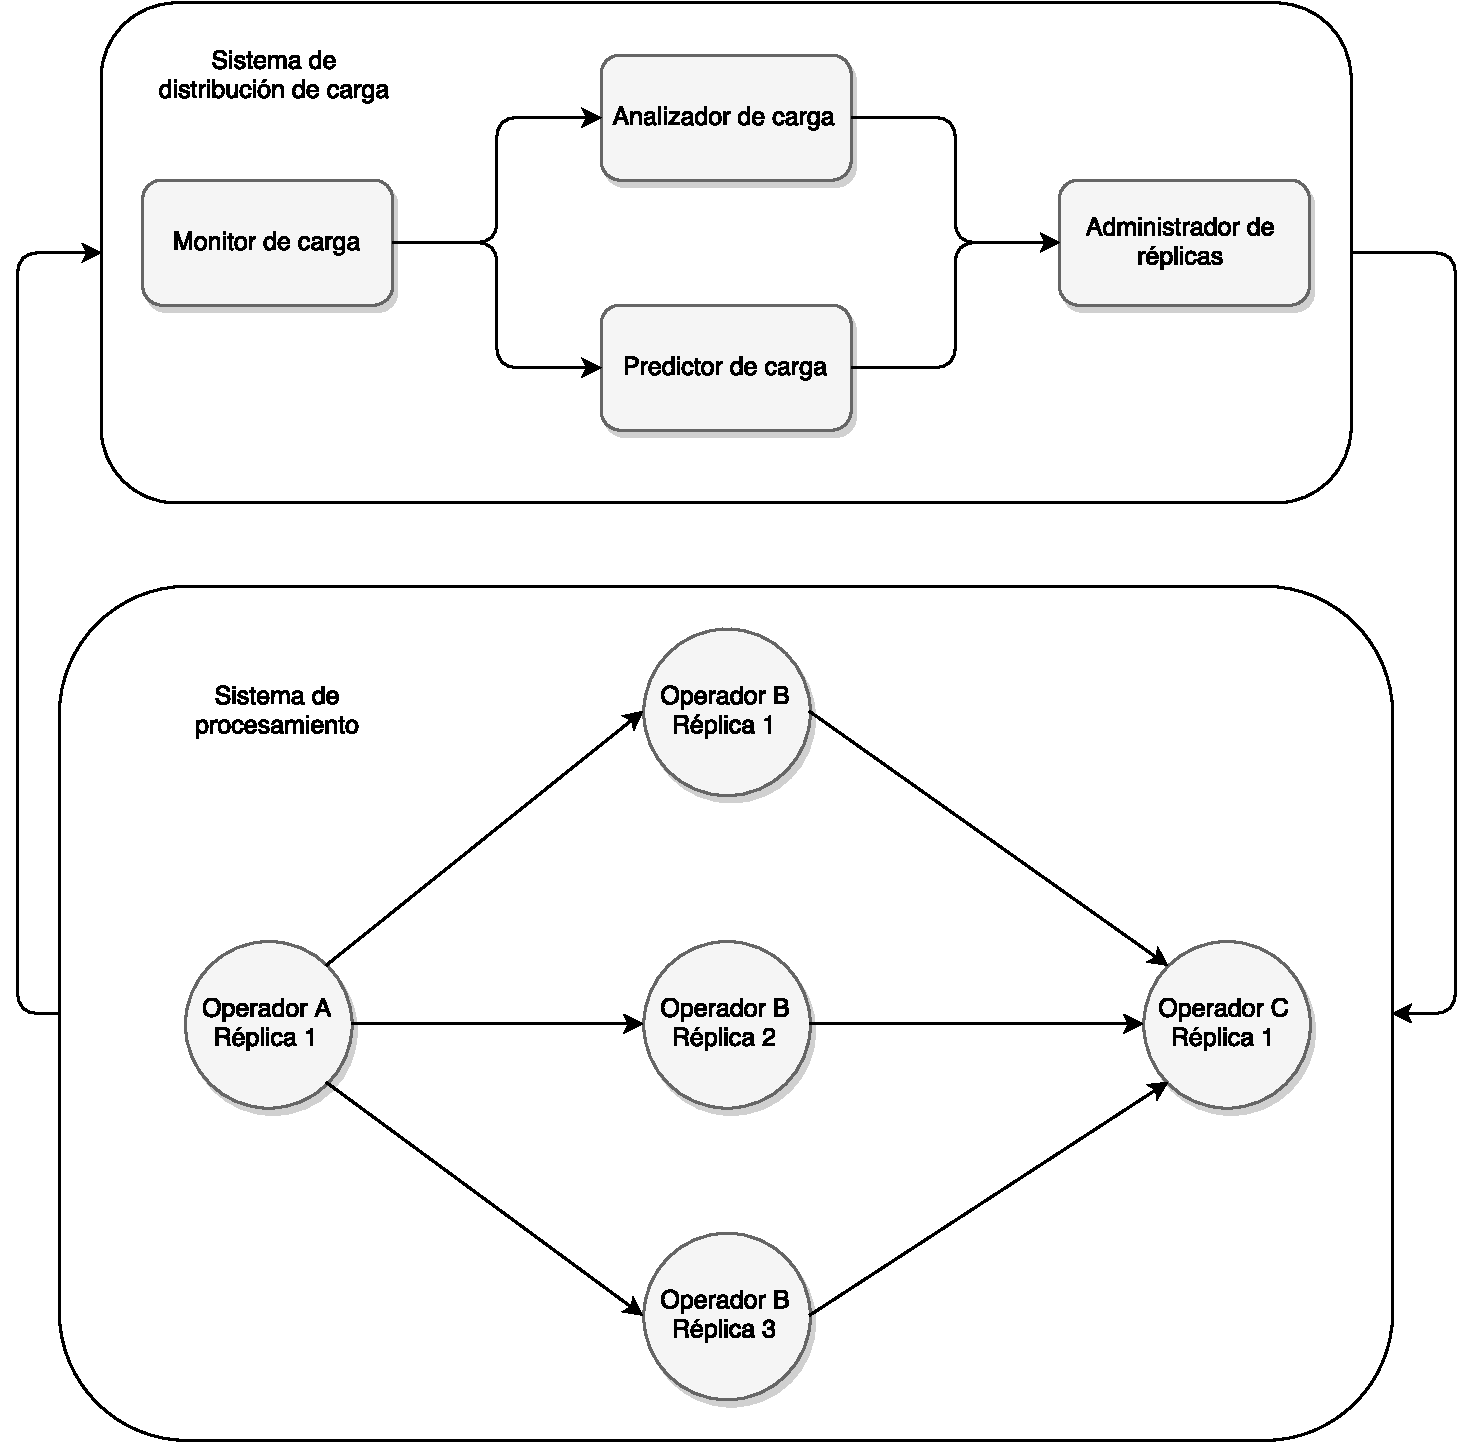
\includegraphics[scale=0.5]{images/Diagrama.pdf}
  \caption{Estructura del sistema de distribución de carga.}
  \label{fig:componentesSistemas}
\end{figure}

\paragraph{Monitor de carga} Está encargado de estar enviado las estadísticas al sistema, ya sea para recolectar las estadísticas para el algoritmo reactivo como el historial para el predictivo.

\paragraph{Analizador de carga} Analiza la cantidad de carga de un operador en un período de tiempo determinado, y respecto a esto se indica el estado del operador. Para esto, se consideró la tasa de rendimiento del operador, y según el valor que posea se determinará el estado, el cual podía ser ocioso, estable o inestable.

\paragraph{Predictor de carga} %Realiza una predicción en base a la historia realizada en cierta ventana de tiempo, utilizando como base las cadenas de Markov. De esta manera, se realiza un cálculo de la distribución estacionaria \citep{Papoulis1984}, para determinar el estado del sistema a futuro y tomar una decisión respecto a esto.
Analiza la historia de un operador en una ventana de tiempo determinada, utilizando como muestra la tasa de rendimiento del operador, para posteriormente realizar una cadena de Markov según los posibles estados del sistema. Posteriormente, para la predicción de la carga del operador, se calculó la distribución estacionaria \citep{Papoulis1984}, el cual va a entregar la probabilidad que el operador se encuentre en cada uno de los posibles estados.

\paragraph{Administrador de réplicas} Se encarga de determinar cual es el algoritmo a utilizar en cada período de tiempo, ya sea reactivo o predictivo, y la administración de las réplicas dado el resultado del algoritmo utilizado.

\section{Recolección de los datos}
%Como se había mencionado anteriormente, el monitor de carga está encargado de recolectar la tasa de rendimiento de cada uno de los operadores, tanto del historial como los datos en el momento. Para esto, se consideró una ventana de tiempo de 1 segundo para la recolección del historial, y 5 segundos para el análisis del operador en el momento.

Como se había mencionado anteriormente, el monitor de carga está encargado de recolectar los datos necesarios para el funcionamiento del sistema de distribución de carga, tanto el historial para el algoritmo predictivo, como la tasa de rendimiento para el algoritmo reactivo. Para esto se consideraron ventanas de tiempo de un segundo para la recolección de cada muestra para el análisis del historia, y cinco segundos para el análisis reactivo del operador.

%Para la recolección del historial se consideraron muestras de 100 datos, esto fue propuesto de esta manera, debido que cada 100 segundos se realiza el algoritmo predictivo, tomando en consideración que cada un segundo recolecta una muestra. La cantidad de muestras fue determinado de esta manera, porque se consideró un número apropiado según lo indicado en la literatura \citep{ching2006markov}.
La recolección de muestras para el historia, se considero un segundo debido que se consideraba un período estable para determinar el comportamiento del operador. Con esto, se iba a poseer una muestra de cien datos cada vez que se realice el algoritmo predictivo, debido que cada cien segundo se va a ejecutar. La cantidad de muestras fue determinado según la literatura, debido que se consideraba un número apropiado para realizar una predicción del operador \citep{ching2006markov}, de tal manera de no existir una deficiencia en la cantidad de muestras para la predicción deseada.

%Analizar con más detalle el tema de mu, porque quizá es erróneo lo descrito aquí
Por otra parte, para la obtención de muestras para el algoritmo reactivo, se consideraron muestras obtenidas en períodos de cinco segundo. La muestra corresponderá a la tasa de rendimiento del operador en ese período, la cual es utilizada por el algoritmo reactivo para determinar el estado del operador según los umbrales propuestos. Dentro de las consideraciones realizadas para la recolección de datos para el algoritmo reactivo, fue considerar que la tasa de servicio ($\mu$) es homogénea con el transcurso del tiempo, debido que los datos procesados lo son, por lo tanto, se considera el valor más alto y ese es considerado en el procesamiento de los datos. 

Cabe destacar que cuando el algoritmo predictivo se ejecuta, no es necesario la recolección de los datos del período, debido que el algoritmo reactivo no será utilizado y sólo considerado datos del momento. Sólo la recolección del historial es realizada en todo momento, dado que estás son guardadas para posteriormente ser analizadas por el algoritmo predictivo.

\section{Algoritmo reactivo}
El diseño del algoritmo reactivo se basó en el análisis del estado del operador en un período determinado, siendo definido su estado por una variable del operador, el cual dependerá del rango en que se encuentre dado los límites que se poseen. En este caso, se analizó según la tasa de rendimiento ($\rho$), donde el estado del operador dependerá del valor que éste posea según los limites establecidos.

En el Algoritmo \ref{alg:reactive} se puede ver el análisis del estado de un operador según su tasa de rendimiento; en el caso que sea mayor a 1, su estado es inestable, menor a 0.5, significa que está en estado ocioso, y sino, significa que está estable. Estos datos posteriormente serán considerados por al administrador de réplicas, el cual analiza el comportamiento que debe tener el sistema según lo indicado por el algoritmo.

\begin{algorithm}[!ht]
	\caption{Algoritmo reactivo del sistema de distribución de carga.}
	\label{alg:reactive}
	\begin{algorithmic}[1]
	\REQUIRE Tasa de procesamiento $\rho$ del operador $\phi$.
	\ENSURE Estado del operador, donde -1 significa estado ocioso, 0 estable y 1 inestable.
	\IF {$\rho_\phi > 1$}
		\RETURN{1}
	\ELSIF {$\rho_\phi < 0.5$}
		\RETURN{-1}	
	\ELSE
		\RETURN{0}
	\ENDIF
	\end{algorithmic}
\end{algorithm}

En la Figura \ref{fig:umbrales} se puede analizar el estado del operador según la tasa de procesamiento de forma visual. En los primeros segundos la tasa del operador es mayor al límite superior, lo cual indica que el sistema es inestable, es decir, el operador posee sobrecarga. Con el transcurso del tiempo, la tasa de rendimiento disminuye, ya sea por una optimización o disminución de la tasa de llegada, por lo que ahora el operador ya no se encuentra sobrecargado, sino se encuentra entre el límite inferior y superior, cuyo rango define al operador como un sistema estable.

\begin{figure}[hb!]
  \centering
    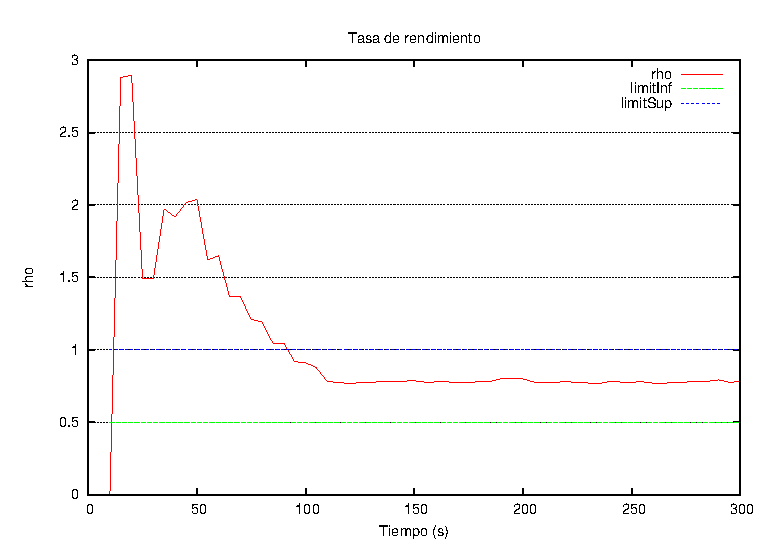
\includegraphics[scale=0.8]{images/Umbrales.eps}
  \caption{Comportamiento de la tasa de procesamiento de un operador.}
  \label{fig:umbrales}
\end{figure}


\section{Algoritmo predictivo}
Para la confección del algoritmo predictivo se realizó un análisis según las cadenas de Markov \citep{ching2006markov}, por lo que se tuvieron que seguir las siguientes condiciones:

\begin{itemize}
	%\item Definir tiempo discretos, los cuales fueran cambiando con el tiempo según un proceso estocástico. Para esto se consideró el cambio del estado del sistema de período a otro, es decir, las transiciones existentes entre cada uno de los estados, ya sea ocioso, estable o inestable, en período de un segundo.
	\item Definir muestras en tiempos discretos, las cuales cambiaran con el tiempo según un proceso estocástico. Las muestras se definieron como la tasa de procesamiento del operador, la cual dependiendo del valor que poseyera, iba a otorgar un estado al operador.
	\item Determinar los estados finitos que se van a utilizar para la conformación de la cadena, que en este caso sería los estados que puede encontrar el operador: ocioso, estable o inestable.
	%\item Una cantidad de muestras considerables para realizar un muestreo que sea representativo según el período analizado. Para la implementación del algoritmo se utilizaron 1. Estas muestras serán independientes unas con otras, por lo que cada cierto período de tiempo se volverá a crear otra cadena de Markov independiente de los datos del pasado.
	\item Una cantidad representativa de muestras para la construcción de la cadena de Markov en el período analizado. Estas muestras serán independientes de un período y otro, por lo que los valores de la cadena de Markov irán cambiando en cada período de tiempo. Para la implementanción del algoritmo, se consideraron cien muestras por cada período, cuyos intervalos eran de cien segundos.
\end{itemize}

%Dato esto, se presentó un cadena de Markov en base a estas bases, como se refleja en la Figura \ref{fig:cadenaMarkovPredictiva}, donde existen tres estados, los cuales pueden ser ocioso, estable o inestable, y poseen ciertas transiciones de un estado a otro, cuyas probabilidades van a estar determinadas por la historia existente en el sistema.

%Dado esto, se construyó una cadena de Markov en base a la transición de un estado a otro del operador según la tasa de rendimiento, donde los tres posibles estados son ocioso, estable o inestable, donde exista una probabilidad de transición entre un estado a otro, cuyos valores estarán determinados por el historial del período analizado.

Tomando las bases anteriores, se diseño una cadena de Markov en base a tres posibles estados: ocioso, estable e inestable, como se demuestra en la Figura \ref{fig:cadenaMarkovPredictiva}. Cada uno de los estados posee una probabilidad de transición hacia algún estado, cuyas probabilidades están definidas por las muestras obtenidas en el período de tiempo analizado.

\begin{figure}[ht!]
  \centering
    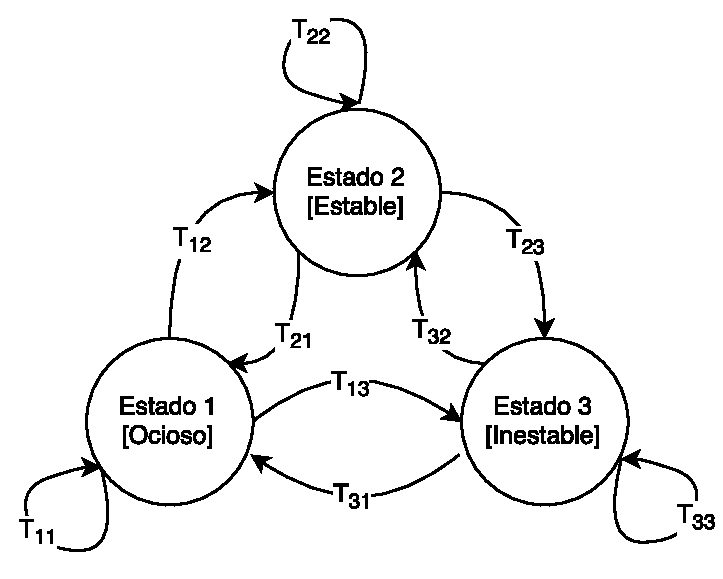
\includegraphics[scale=0.75]{images/CadenaMarkovPredictiva.pdf}
  \caption{Cadena de Markov dado el modelo propuesto del sistema.}
  \label{fig:cadenaMarkovPredictiva}
\end{figure}

%Por lo tanto, para cada operador existe una cadena de Markov según la historia existente en una ventana de tiempo. Para la generación de esta cadena de Markov, se puede ver en el Apéndice \ref{apendice:matrizTransicion} el algoritmo que crea la matriz de transición según el historial del operador, la cual corresponde a la tasa de rendimiento recolectada cada un segundo en la última ventana de tiempo del operador analizado. En la Ecuación \ref{eq:matrizTransicionPredictive} se puede ver la matriz de transición que se obtiene de la cadena de Markov de la Figura \ref{fig:cadenaMarkovPredictiva}, la cual posee una probabilidad de transición desde cada uno de los estado a otro existente.

Por lo tanto, para cada operador se construirá una cadena de Markov según el historial obtenido en la ventana de tiempo. Para la conformación de la cadena de Markov se consideraron las muestras de la historia, por lo que la transición de una muestra a otra presentaba un transición, las cuales dieron origen a la matriz de transición. En el Anexo \ref{apendice:matrizTransicion} se puede ver el algoritmo que se empleó para construir la matriz de transición. En la ecuación \ref{eq:matrizTransicionPredictive} se muestra la matriz de transición que se obtiene de la cadena de Markov de la Figura \ref{fig:cadenaMarkovPredictiva}.

\begin{equation} \label{eq:matrizTransicionPredictive}
	P =
	\begin{bmatrix}
		T_{1,1} & T_{1,2} & T_{1,3} \\
		T_{2,1} & T_{2,2} & T_{2,3} \\
		T_{3,1} & T_{3,2} & T_{3,3}
	\end{bmatrix}	
\end{equation}

%Teniendo la matriz de transición de la cadena de Markov de un operador, se puede calcular la distribución estacionaria, la cual indica la probabilidad que a largo plazo se encuentre el sistema en cierto estado, ya sea ocioso, estable o inestable. Para el cálculo de esta, se utiliza la ecuación de Chapman-Kolmogórov \citep{Papoulis1984} expuesta en la subsección \ref{subsec:cadenaMarkov}.
Obtenida la matriz de transición se puede calcular la distribución estacionaria de la cadena de Marjov, la cual indica las probabilidades que en el futuro se encuentra el operador esté en cada uno de los posibles estados, ya sea ocioso, estable o inestable. Para el cálculo de esto, se utiliza la ecuación de Chapman-Kolmogórov \citep{Papoulis1984} descrita en la subsección \ref{subsec:cadenaMarkov}.

El Algoritmo \ref{alg:distEstacionaria} describe el cálculo de la distribución estacionaria, cuya entrada es la matriz de transición de un operador del SPS. 

Antes de realizar el cálculo, era importante analizar si efectivamente existían transiciones en todos los estados, debido que existía la posibilidad que no hubiera alguna transición a algún estado en un período de tiempo. Por ejemplo, podría ser que en cierto período nunca se ha encontrado ocioso el sistema, pero si estable e inestable. Como el cálculo de la distribución estacionaria requiere un estado de inicio, se verificó si efectivamente existía o no el estado, y en caso no existir, el estado de inicio será alguno existente.

%Al realizar las iteraciones correspondientes al cálculo, se proporcionó como entrada la cantidad que se estimaba necesario. Es importante destacar que entre mayor cantidad de iteraciones, mayor precisión existe en el cálculo, pero mayor es el tiempo de espera.
La cantidad de iteraciones que debe realizarse para el cálculo correspondiente, se proporcionó como entrada del algoritmo según lo que se estimaba necesario. Es importante destacar que entre mayor cantidad de iteraciones, mayor precisión en el valor, pero mayor es el tiempo de cómputo. Debido a esto, es que se trató de considerar un punto medio, de tal manera que tuviera bajo margen de error, pero no fueran alto su tiempo de ejecución, siendo 100.000 la cantidad de iteraciones escogida para la implementación.

\begin{algorithm}[!ht]
	\caption{Cálculo de la distribución estacionaria de la cadena de Markov de un operador $\phi$.}
	\label{alg:distEstacionaria}
	\begin{algorithmic}[1]
	\REQUIRE $\Gamma$ Matriz de transición del operador $\phi$ y $\upsilon$ cantidad de iteraciones deseadas.
	\ENSURE $\Delta$ Distribución estacionaria de la cadena de Markov del operador $\phi$.
	\STATE $i \leftarrow 0$ \COMMENT {Estado inicial de iteración}
	\FOR {$j=1$ a $3$}
		\IF {$\Gamma_{j,x} = 0 ; x={1,2,3}$}
			\STATE {$i \leftarrow j$}
		\ENDIF
	\ENDFOR
	
	\STATE $\tau \leftarrow Arreglo[3]$ \COMMENT {Contador para la normalizaci\'on de los datos}
	\FOR {$k=0$ a $\upsilon$}
		\STATE $u = randomUniform(0,1)$
		\STATE $\sigma = 0$
		\FOR {$j=0$ a $3$}
			\STATE $\sigma = \sigma + \Gamma_{i,j}$
			\IF {$u \leqslant  \sigma$}
				\STATE $\tau_{j}++$
				\STATE $i \leftarrow j$
				\STATE \textbf{break}
			\ENDIF
		\ENDFOR
	\ENDFOR

	\STATE $\Delta \leftarrow Arreglo[3]$ \COMMENT {Distribución estacionaria de la cadena de Markov del operador $\phi$}
	\FOR{$k=0$ a $3$}
		\STATE $\Delta_{k} \leftarrow \nicefrac{\tau_{k}}{\upsilon}$
	\ENDFOR	
	
	\RETURN $\Delta$
	
	\end{algorithmic}
\end{algorithm}

%Obtenida la distribución estacionaria, se procese a analizarla el comportamiento de esta. Para esto, se consideró que era importante que la probabilidad entre estados tuviera una desviación estándar superior a 0.25, de tal manera que se trabajen con probabilidad que no posean incertidumbre en su comportamiento a futuro. En el Algoritmo \ref{alg:predictive} se puede ver el análisis que se realiza a la distribución estacionaria, ya sea por el comportamiento estadístico o de estado del sistema, donde retornará el estado a futuro del operador, dada la probabilidad más alta de la distribución estacionaria, si es que supera la desviación estándar propuesta. Se tomó en consideración que el primer estado es el ocioso, el segundo estado es el estable y el tercer estado es el inestable.
Obtenida la distribución estacionaria, se procede a analizar las probabilidades obtenidas y como influye al operador. Para esto, se consideró que las probabilidades tuvieron entre ellas una desviación estándar superior a 0.25, debido que si esto se cumple, la probabilidad mayor de la distribución estacionaria no posee incertidumbre, porque en caso que no supere la desviación estándar, puede ser que dos probabilidades sea muy parecidas y la probabilidad no sea un comportamiento determinante. En el Algoritmo \ref{alg:predictive} se describe el análisis que se realiza a la distribución estacionaria, siendo en primer lugar el análisis estadístico de las probabilidades, y segundo la obtención del estado con mayor valor de las probabilidades, retornando finalmente el estado del operador. Cabe destacar que el primer estado se consideró ocioso, el segundo estable, y el tercero inestable.

\begin{algorithm}[!ht]
	\caption{Algoritmo predictivo del sistema de distribución de carga.}
	\label{alg:predictive}
	\begin{algorithmic}[1]
	\REQUIRE$\Delta$ Distribución estacionaria de la cadena de Markov del operador $\phi$.
	\ENSURE Estado a futuro del operador, donde -1 significa estado ocioso, 0 estable y 1 inestable.
	\IF {$\sigma(\Delta_1,\Delta_2,\Delta_3) > 0.25$ \COMMENT {Desviaci\'on est\'andar de las probabilidades de la distribuci\'on estacionaria}} 
		\STATE $i \leftarrow getStateMax(\Delta)$ \COMMENT {Obtención del estado con mayor probabilidad}
		\IF {$i=1$}
			\RETURN -1
		\ELSIF {$i=2$}
			\RETURN 0			
		\ELSE
			\RETURN 1
		\ENDIF
	\ENDIF
	
	\RETURN 0
	
	\end{algorithmic}
\end{algorithm}

\section{Administración del sistema}

El último componente del sistema es el administrador de réplicas, cuya función es administrar la cantidad de réplicas en cada uno de los operadores según los recursos disponibles por parte del sistema y según el estado que adopte un operador, ya sea a futuro o en el momento.

%Para esto, se diseño un administrador que se ejecutara según el período que se encuentra el algoritmo reactivo o predictivo, donde cada período es de 19 ejecuciones del algoritmo reactivo y 1 del algoritmo reactivo. Esto fue pensando dado que cada cien segundos se poseían las muestras suficientes para el análisis del algoritmo predictivo, por lo tanto, cada ejecución del algoritmo reactivo iba a ser cada cinco segundos, de esa manera al segundo cien iba a realizarse en vez del algoritmo reactivo, el predictivo ya que posee la cantidad suficiente de muestras para su análisis.
Para esto, se diseño un administrador que ejecutara un tipo de algoritmo (reactivo o predictivo) según el período del ciclo que se encuentre el sistema. Cada ciclo posee 20 períodos, donde los primeros 19 corresponde al algoritmo reactivo y el último corresponde al algoritmo predictivo. Cada período posee un intervalo de 5 segundos, de esta manera, cada ciclo tendrá un intervalo de 100 segundos, la cantidad necesaria para obtener las muestras para el algoritmo reactivo, suponiendo que cada muestra es obtenida en 1 segundo.

En el Algoritmo \ref{alg:administracion} está el procedimiento de administración, donde primero analiza que tipo de algoritmo debe ejecutar según el período del ciclo. En caso de realizarse el reactivo, se analiza si existen dos alertas consecutivas del mismo estado del sistema, ya sea ocioso o inestable, y de ser así, realizar una modificación a la cantidad de réplicas del operador. Por otra parte, de ejecutarse el módulo predictivo, se analiza cual fue la predicción, por lo que si es ocioso disminuirá la cantidad de réplicas y si es inestable las aumentará. Como el proceso de predicción se realiza con menor frecuencia y posee mayor cantidad de cómputo, se considero que debía crear o remover mayor cantidad de réplicas que en el módulo reactivo, aprovechando así el análisis de la historia del operador.

\begin{algorithm}[!hb]
	\caption{Administración de réplicas de un operador $\phi$ dado su comportamiento en el sistema de distribución de carga.}
	\label{alg:administracion}
	\begin{algorithmic}[1]
	\REQUIRE Operador $\phi$ a analizar y $\iota$ período en que se encuentra el sistema de distribución de carga.
	\ENSURE Cantidad de réplicas a modificar del operador.	
	
	\IF {$\iota \mod{20} \neq 0 $}
		\STATE $\delta_{\iota} \leftarrow AlgoritmoReactivo(\phi)$
		\IF {$\delta_{\iota}$ \AND $\delta_{\iota-1}$ son estado inestable}
			\IF {No excede la cantidad máxima de réplicas en el sistema}
				\RETURN Crear una réplica del operador $\phi$
			\ENDIF
		\ELSIF {$\delta_{\iota}$ \AND $\delta_{\iota-1}$ son estado ocioso}
			\RETURN Remover una réplica del operador $\phi$
		\ENDIF 
	\ELSE
		\STATE $\delta_{\iota} \leftarrow AlgoritmoPredictivo(\phi)$
		\IF {$\delta_{\iota}$ es estado inestable}
			\IF {No excede la cantidad máxima de réplicas en el sistema}
				\RETURN Crear cinco réplicas del operador $\phi$
			\ENDIF
		\ELSIF {$\delta_{\iota}$ es estado ocioso}
			\RETURN Remover cinco réplicas del operador $\phi$
		\ENDIF
	\ENDIF
	
	\RETURN No hacer nada al operador $\phi$
	
	\end{algorithmic}
\end{algorithm}

Dentro de las consideraciones que se tuvieron para el diseño del administrador, fue la cantidad máxima de réplicas que podían realizarse. Dado que una de las limitantes de este trabajo fue que sólo se utilizó una máquina, la cantidad de recursos son limitados, por lo que aumentar la cantidad de réplicas indefinidamente iba a generar una sobrecarga en los recursos disponibles por parte de la máquina, habiendo fallas en el funcionamiento del SPS.
\chapter{Experimentos y evaluación}
\label{cap:experimentos}

\section{Implementación del sistema}
%Acá hay que hablar de todo lo que implementaste a grandes rasgos (detalles Anexo), modelo, manejo de réplicas, etc. Redactar de nuevo

Para la implementanción del sistema propuesto, se utilizó como base el motor de procesamiento de \textit{stream} S4 \citep{s4}, cuyo modelo fue explicado en la sección \ref{sec:SPS}. El funcionamiento del sistema de distribución de carga propuesto se desarrolló en Java, donde se modificó en el código fuente de S4, para incluir las funciones de este producto, de tal manera que fuera automático y transparente para el usuario del SPS.

El sistema diseñado fue añadido al proyecto S4, siendo una paquete denominado \textit{monitor} que contenía las clases \textit{S4Monitor}, \textit{MarkovChain}, \textit{MonitorMetrics}, \textit{StatusPE} y \textit{TopologyApp}. La primer clase correspondía a las funcionalidades del sistema de monitoreo, ya sea la recepción de los datos del sistema, ejecución del algoritmo reactivo o predictivo y administración de las réplicas de cada operador. La segunda clase hacía alusión al modelo de cadena de Markov implementando por el algoritmo predictivo, donde posee tanto la conformación de la matriz de transición como el cálculo de la distribución estacionaria. La tercera clase se utilizó para recolectar las estadísticas de cada operador, y poder analizar los experimentos. Finalmente, la cuarta y quinta clase fueron utilizadas para la implementación del sistema de monitoreo, siendo la primera el estado de cada PE y el segundo la topología que poseía el grafo creado por el usuario, los cuales pueden verse con más detalle en el Anexo \ref{apendice:clases}.

Para la ejecución del SPS conjunto con el monitor, se debe en primer lugar registrar los PEs. Para esto, se implementó una función que tenga como parámetro dos PEs, donde el primero es el PE emisor y el segundo el receptor. Esta información es importante para obtener la topología del grafo, dado que con esto se puede realizar un análisis del rendimiento de los PEs.

Además de lo anterior, para el análisis de cada uno de los PEs, se añadió los atributos de cantidad de eventos entrantes y salientes cada un segundo y cinco segundos en la clase del PE. Esto fue utilizado posteriormente para las estadísticas deseadas para el algoritmo reactivo y predictivo. La tasa de llegada es considerada desde el momento que se recibe el evento desde el PE emisor, y la tasa de servicio es considera desde el momento que se termina de realizar la ejecución de la tarea en el PE. Además, se agregó un atributo booleano, el cual indica si el PE puede aumentar o disminuir la cantidad de réplicas que posee al iniciar el sistema.

Posteriormente, para el funcionamiento del sistema de distribución de carga se procedió a ejecutar dos tareas en la aplicación de S4: una tarea que guarde las muestras para el historial del operador y otra que envíe las estadísticas del operador, las cuales poseían un intervalo de ejecución de 1 y 5 segundos respectivamente. La primera tarea analiza cada uno de los PEs, tomando en consideración las estadísticas de eventos entrantes y salientes, los cuales darán origen a la tasa de llegada ($\lambda$) y servicio ($\mu$), para que posteriormente se calcule la tasa de rendimiento en la ventana de tiempo analizada, guardando así la muestra en el historial. La segunda tarea obtiene las estadísticas de cada uno de los PEs, ya sea la tasa de llegada ($\lambda$) y servicio ($\mu$), dado los eventos entrantes y saliente, cantidad de eventos totales e historial del PE, los cuales son enviados al monitoreo de carga, para posteriormente ejecutar el algoritmo que corresponda según la ventana de tiempo, y finalmente realizar la administración de réplicas para aumentar o disminuir las réplicas necesarias en cada operador según lo necesario. El código de la implementanción se puede observar en el Anexo \ref{apendice:codigoFuenteS4}.

Debido al funcionamiento de los SPS, existe una fuente de datos, por lo tanto, para la correcta sincronización de las estadísticas, se procedió a realizar una espera por parte del monitor hasta que la fuente de datos esté lista para enviar los datos. Esta implementanción se puede ver en el Anexo \ref{apendice:codigoFuenteS4}, conjunto con las dos tareas que debe ejecutar después que la fuente de datos avisa de su inicialización.

En el caso del envío de las estadísticas, después de ser enviadas, se consulta el estado de cada uno de los operadores, y en caso de ser necesario, se realiza las modificaciones necesarias en el sistema, ya sea de crear o eliminar réplicas de un operador. En el caso de crear réplicas, lo que se realiza es consultar la cantidad de réplicas que dijo que deben existir por parte del administrador de réplicas, y en caso de poseer un número de réplicas mayor que el existente por el PE, se procede a crear la cantidad de réplicas faltantes. Por otra parte, en caso de que el número sea menor, procede a terminar la ejecución del PE y posteriormente elimina la cantidad de réplicas sobrantes. En caso que el operador que se haya identificado con el atributo único, significa que no puede aumentar ni disminuir la cantidad de réplicas asignadas a éste. Los códigos de crear o eliminar replicas se encuentra adjuntos en el Anexo \ref{apendice:codigoFuenteS4}.

Dado que en el diseño se propuso un mecanismo de balance de carga basado en la técnica de replicación, fue necesario modificar S4, de manera de poder manejar las réplicas para los operadores. Se implementó el SPS de tal manera de poder manejar un algoritmo que escogiera la réplica que tuviera menor tamaño en la cola de espera al momento de enviar un dato, y así siempre escoger al operador con menor carga, y en caso que posean el mismo tamaño, utilizar la primera réplica disponible.

En la Figura \ref{fig:distCarga} se explica gráficamente la distribución de la carga. En la parte (a) el operador A envía un evento al operador B, el cual posee tres réplicas, cuyas menores colas están en la réplica 2 y 3, como son iguales las colas de estas réplicas, se escoge la primera réplica disponible, es decir, la réplica 2. Posteriormente, como la réplica 2 aumento su cola, la réplica 3 es la que posee menor cantidad de cola, como se demuestra en la parte (b), por lo tanto, es la réplica candidata a recibir el dato enviado. Y finalmente, en la parte (c) todas las réplicas posee el mismo tamaño de la cola, por lo tanto, se procede a enviar a la primera réplica.

\begin{figure}[!ht]
	\centering
		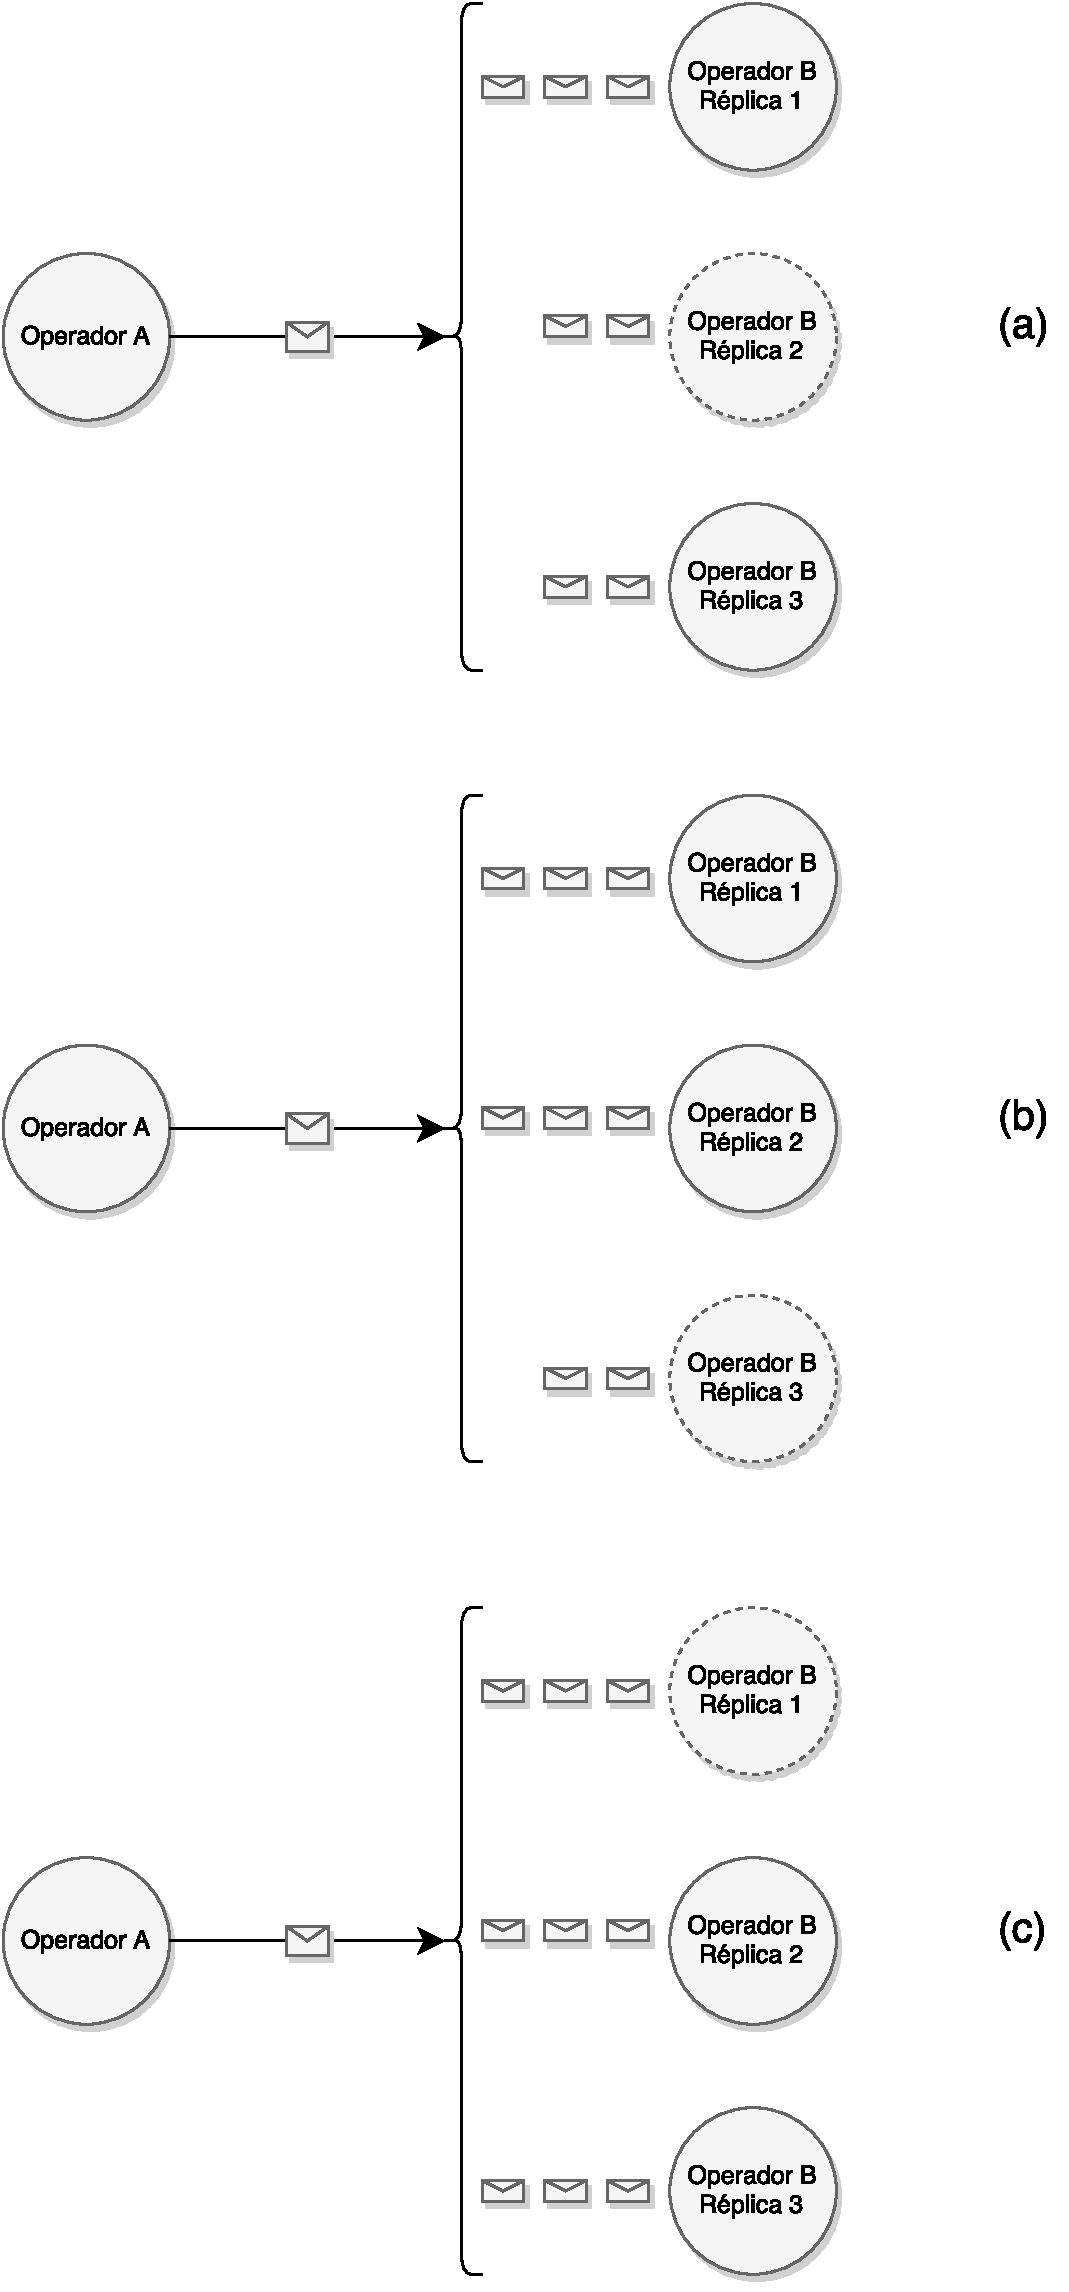
\includegraphics[scale=0.55]{images/DistribucionCarga.pdf}
	\caption{Distribución de la carga entre las réplicas.}
	\label{fig:distCarga}
\end{figure}

En el Algoritmo \ref{alg:distCarga} está descrito la distribución de carga planteada anteriormente, la cual fue implementada en S4 para realizar los experimentos según lo diseñado en el planteamiento de los algoritmos.

\begin{algorithm}[!ht]
	\caption{Distribución de carga entre las réplicas de un operador.}
	\label{alg:distCarga}
	\begin{algorithmic}[1]
	\REQUIRE Evento $\epsilon$ y operador $\phi$.
	\ENSURE Envío del evento a la réplica disponible del operador $\phi$.
	\STATE $\theta \leftarrow minTamanoCola(\phi)$ \COMMENT Se escoge la réplica que posea menor cola
	\STATE $envioEvento(\epsilon,\theta$)
	\end{algorithmic}
\end{algorithm}

\section{Diseño de los experimentos}
Para los experimentos se diseñaron tres aplicaciones, una que realiza operaciones con estado, otra que no, y otra que es sintética. En el caso que la aplicación posea estado, significa que el operador guarda variables con el transcurso del tiempo, las cuales van a ser entregadas cada cierto tiempo o al finalizar la ejecución del sistema. Un ejemplo de esto, es un sistema que cuenta las palabras de un texto y que envié la cantidad de palabras contadas cada cierta ventana de tiempo. Por otra parte, la aplicación sintética se refiere a un sistema cuyos operadores sólo generan tiempo de demora artificial, en el caso de este experimento, se dejo durmiendo la hebra asignada al operador un período determinado de tiempo.

Para la generación del \textit{stream} de la fuente de datos para la primera y segunda aplicación, se utilizaron datos de muestra utilizados fueron \textit{tweets} recolectados entre los días 27 y 28 de Febrero y 1 y 2 de Marzo de 2010, tanto en inglés, portugués y español, cuya información correspondía a la interacción entre los usuarios debido al terremoto ocurrido el 27 de Febrero en el territorio Chile.

Por otra parte, el envío de los datos anteriores se realizó de dos maneras: constante y variable. La primera forma consiste en enviar 100 eventos por segundo constantemente. En cambio, la segunda forma consiste en enviar 50 eventos por segundos el primer tercio del experimento, para luego aumentar a 75 eventos por segundo, los primeros 120 segundos del segundo tercio, y seguir aumentando a 100 eventos por segundo, para posteriormente volver a 75 eventos por segundos los últimos 120 segundos del segundo tercio, y finalmente, disminuir a 50 eventos por segundos el último tercio de la ejecución.

%Estos datos fueron enviados de dos formas: el primero de forma uniforme, enviado 100 eventos por segundos constantemente, y la segundo de forma variable, enviado 50 eventos por segundo el primer tercio de la ejecución del programa, para posteriormente aumentarla a 100 eventos por segundo en el segundo tercio, y finalmente disminuirla a 50 eventos por segundo en el último tercio de la ejecución del programa.

\subsection{Análisis de \textit{tweets} en escenarios de desastres naturales}
La primera aplicación fue orientada a un caso de desastres naturales, donde se generó un grafo que pudiera realizar un filtrado de palabras y análisis de los datos. Ninguno de los operadores posee estado, por lo tanto son independientes. Para la duración de esta prueba se consideró un tiempo de 70 minutos.

La aplicación consta del flujo de datos, cuyos datos serán la muestra de \textit{tweets} de prueba, y cuatro operadores, los cual son denominados \textit{Stopword}, \textit{Language}, \textit{Counter} y \textit{MongoDB}.

\paragraph{Stopword}: está encargado de analizar el \textit{tweet} y remover las palabras no relevantes para el análisis de éste, basado en una bolsa de palabras, cuyas palabras se llaman \textit{stopwords}. De esta manera, se puede analizar el texto usando las palabras más representativas de éste y así entregar información más precisa.

\paragraph{Language}: está encargado de analizar el lenguaje existente en el \textit{tweet}, para esto se utilizó una librería \textit{Apache Tika} \citep{mattmann2011tika}. Con ésta se puede realizar un filtro del idioma de los tweets, de tal manera que en caso de ser requerido, sólo continúen los de un idioma en específico, en nuestro caso el español.

\paragraph{Counter}: está encargado de contar e indicar la cantidad de palabras que existen en el \textit{tweet} según una bolsa de palabras proporcionada por el programador. Para esta prueba se utilizó una bolsa de 26.000 palabras en español. Con esto se podría realizar un análisis de los \textit{tweets} que poseían mayor cantidad de palabras claves asociados a una temática o evento en particular.

\paragraph{MongoDB}: está encargado de guardar en la base de datos el evento según los atributos que éste posea, ya sea por el \textit{tweet} original, sin \textit{stopword}, idioma y cantidad de palabras claves existentes en él. Para esto, se utilizó el motor de base de datos no relacional \textit{MongoDB} \citep{chodorow2013mongodb}.

En la Figura \ref{fig:primeraAplicacion} se muestra un ejemplo de la aplicación con sus distintos operadores y relaciones. Las flechas muestran la dirección del flujo de datos emitido por la fuente y los operadores.

\begin{figure}[!hb]
	\centering
		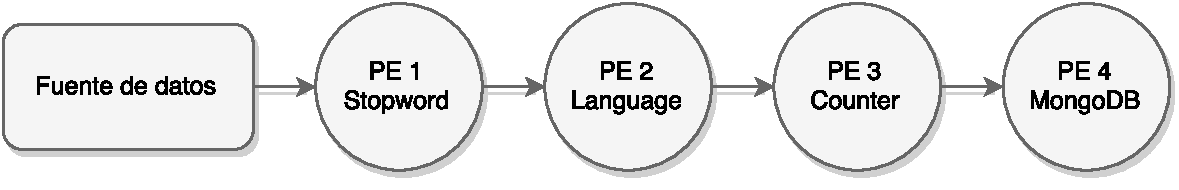
\includegraphics[scale=0.75]{images/App1.pdf}
	\caption{Primera aplicación de prueba.}
	\label{fig:primeraAplicacion}
\end{figure}

\subsection{Contador de palabras en muestras de textos}
La segunda aplicación consiste en un contador de palabras, el cual cuenta la cantidad de veces que se repite una palabra en un conjunto de datos según una bolsa de palabras establecida por el usuario. Esta aplicación se considera con estado, debido que debe existir un contador en el operador, de tal manera de contar la cantidad de veces que se repite cierta palabra de la bolsa de palabras en los datos entrantes. Con esta aplicación es posible analizar posteriormente las palabras más frecuentes emitidas por los usuarios de la red social según un listado de palabras claves. Para la duración de esta prueba se consideró un tiempo de 70 minutos.

La aplicación consta del flujo de datos, cuyos datos serán la muestra de \textit{tweets} de prueba, y tres operadores, denominados \textit{Split}, \textit{Counter} y \textit{Merge}.

\paragraph{Split}: está encargado de dividir el \textit{tweet}, y enviar un arreglo con las palabras que poseía este texto al operador \textit{Counter}.

\paragraph{Counter}: está encargado de guardar las estadísticas de los contadores de cada palabra, es decir, en el momento que reciba un evento, este analiza las palabras que posee y aumenta el contar de la palabra en el operador. Las estadísticas son enviadas cada 10 segundos al operador Merge, de tal manera de no enviar flujo constante al siguiente operador y generar mayor cantidad de carga.

\paragraph{Merge}: está encargado de unir las distintas estadísticas enviadas por las distintas réplicas del operador Counter.

En la Figura \ref{fig:segundaAplicacion} se muestra un ejemplo de la segunda aplicación con sus distintos operadores y sus relaciones, de igual manera que en el caso anterior, las flechas reflejan el flujo de datos. Cabe destacar que el único operador que puede replicarse es el \textit{Counter}, debido que el operador \textit{Split} y \textit{Merge} son operadores que soportan la replicación del operador \textit{Counter}, como se explicó en las técnicas de balance de carga en la subsección \ref{sec:fisionBC}.

\begin{figure}[!hb]
	\centering
		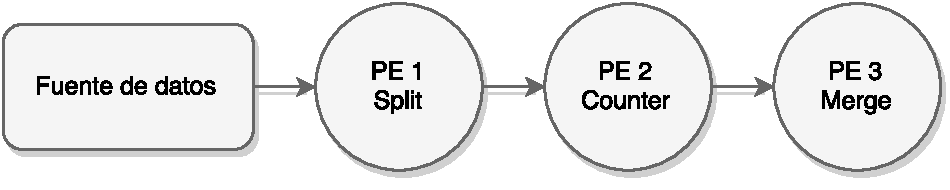
\includegraphics[scale=0.75]{images/App2.pdf}
	\caption{Segunda aplicación de prueba.}
	\label{fig:segundaAplicacion}
\end{figure}

\subsection{Aplicación sintética}
La tercera aplicación consta de tres operadores, los cuales duermen a la hebra asignada al operador un determinado período de tiempo. De esta manera, se genera un tiempo de espera artificial, realizando un operador sintético, de tal manera que pueda simular el comportamiento de un operador real.

La tabla \ref{tab:app3-time} muestra el período de tiempo que duerme cada PEs a su hebra asignada. Los tiempos que se consideraron para esta prueba es para generar una sobrecarga en el primer y segundo operador, de tal manera que después afectarán al tercer operador. Para la duración de esta prueba se consideró un tiempo de 15 minutos.

\begin{table}[!ht]
\centering
\begin{tabular}{| c | c |}
\hline
PE & Tiempo (ms) \\ \hline
1 & 20 \\
2 & 30 \\
3 & 15 \\\hline
\end{tabular}
\caption{Período de tiempo que duerme la hebra asignada al PE.}
\label{tab:app3-time}
\end{table}

En la Figura \ref{fig:terceraAplicacion} se muestra un ejemplo de la tercera aplicación con sus distintos operadores y sus relaciones, de igual manera que en los casos anteriores, las flechas reflejan el flujo de datos.

\begin{figure}[!hb]
	\centering
		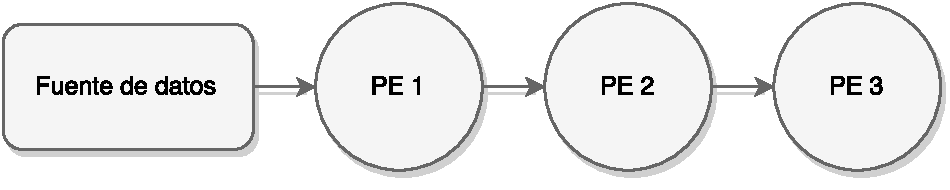
\includegraphics[scale=0.75]{images/App3.pdf}
	\caption{Tercera aplicación de prueba.}
	\label{fig:terceraAplicacion}
\end{figure}

\section{Evaluación}

Para la ejecución de los experimentos, se utilizó un servidor con sistema operativo Ubuntu 14.04.2 LTS, cuyo procesador es un Intel\textregistered Xeon\textregistered CPU E5-2650 v2 de 2.60GHz y con 32 GB de RAM. Cabe recalcar, que el lenguaje de programación fue Java, debido a la integración del sistema propuesto en el SPS utilizado, el cual fue S4. La configuración de la configuración de S4 está detallada en el Anexo \ref{apendice:config-comm-S4}.

La recolección de estadísticas fue realizada cada 5 segundos, por lo que desde ahora se hablará período un intervalo de tiempo de 5 segundos entre cada recolección de las estadísticas.

\subsection{Primera aplicación}
En la primera aplicación se procedió a realizar cuatro experimentos, donde cada par era una comparación del experimento con y sin uso del monitor. Las dos primeras se utilizó flujo constante de la fuente de datos, y las dos segundas un flujo dinámico de la fuente de datos.

Para el análisis de los experimento se consideró la cantidad promedio de eventos procesados en un período, la cantidad total de eventos procesados y las estadísticas de cada PE en el transcurso de la ejecución de la aplicación.

Para analizar el comportamiento del sistema en el primer y segundo experimento, se procedió a estudiar las estadísticas de cada uno de los PEs. En la Figura \ref{fig:app1-uniform-statusStopwordPE-cm} y \ref{fig:app1-uniform-statusStopwordPE-sm} se muestran las estadísticas del primer operador del grafo, con y sin monitoreo en la carga de los operadores respectivamente. En la tasa de llegada ($\lambda$) se puede observar como en el primer gráfico es constante, pero no así en el segundo gráfico, debido que en el segundo 2600 surge una disminución del flujo de datos. Esto se debe a la acumulación de eventos en el \textit{buffer}, por lo que se genera cola en el PE, lo cual impide almacenar mayor cantidad de eventos, dado que la cantidad de eventos que se procesan es menor que la cantidad de eventos que llegan. Por lo tanto, al llenarse el \textit{buffer}, no puede seguir almacenando eventos en la cola, siendo éste bloqueado, habiendo una cola constante como se puede apreciar.

Por otra parte, la tasa de rendimiento de la Figura \ref{fig:app1-uniform-statusStopwordPE-cm} se estabiliza dentro de los primeros 100 segundos, debido que el sistema de distribución de carga detectó una sobrecarga en el operador y replicó el operador, a diferencia de la Figura \ref{fig:app1-uniform-statusStopwordPE-sm}, en el cual el operador posee una tasa de rendimiento estable que bordea entre 1 y 2, hasta el segundo 2600, donde disminuye debido que la tasa de llegada es menor. Cabe destacar que en este operador se encontró una sobrecarga, debido que posee un alto costo computacional, debido que existe una gran cantidad de palabras que debe analizar con cada una de las palabras del texto, por lo que se hace necesario otra réplica en el sistema.

En la Figura \ref{fig:app1-uniform-statusLanguagePE-cm} y \ref{fig:app1-uniform-statusLanguagePE-sm} se puede ver el siguiente operador del gráfico, el cual no tiene mayor inconveniente, a excepción del segundo 2400, donde el sin monitoreo disminuye considerablemente la tasa de procesamiento del PE. Si analizamos la Figura \ref{fig:app1-uniform-statusStopwordPE-sm} y \ref{fig:app1-uniform-statusLanguagePE-sm}, empiezan aproximadamente desde el rango de tiempo (2400s,2600s) los problemas de procesamiento de los operadores, por lo tanto, se puede deducir que si el problema surge en un operador no es un problema aislado, sino que también influye a los siguientes operadores.

Se puede observar como con el transcurso de los primeros 100 segundos en la Figura \ref{fig:app1-uniform-statusCounterPE-cm}, fue aumentando la cantidad de réplicas hasta llegar a 5, el cual fue su óptimo, para ir procesando la cantidad de eventos y disminuir la cola existente en el sistema. Esto en contra posición a la Figura \ref{fig:app1-uniform-statusCounterPE-sm}, donde la inexistencia de replicación, genera una cola la cual se mantiene constante en el segundo 2400. 

Finalmente, se encuentra el último operador, el cual no presenta grandes inconvenientes tanto en la Figura \ref{fig:app1-uniform-statusMongoPE-cm} y \ref{fig:app1-uniform-statusMongoPE-sm}, esto debido que el tiempo de procesamiento es bajo, y nunca llega una cantidad de eventos considerable para existir una sobrecarga en éste. Además es importante destacar que en la Figura \ref{fig:app1-uniform-statusMongoPE-sm} llega una menor tasa de llegada, exactamente un $83,827\%$ menos de eventos que un SPS ejecutado con el sistema de distribución de carga.

Por otra parte, también se analizó la cantidad promedio de eventos procesados en cada período, la cual está graficada en la Figura \ref{fig:app1-uniform-cm-avgEventProcess} y \ref{fig:app1-uniform-sm-avgEventProcess}. Como se puede apreciar, en los primeros 50 segundos se puede ver una mejora considerable en la cantidad de eventos procesados, donde posteriormente se procesan aproximadamente 480 eventos por período con monitoreo, a diferencia del SPS sin monitoreo, que procesa 90 eventos por período aproximadamente, habiendo una mejora del $615,38\%$. Esta mejora se debe al factor de la replicación de los operadores que posee mayor sobrecarga, por lo que al aumentar la cantidad de réplicas, aumenta la tasa de procesamiento, lo significa mayor cantidad de flujo para el próximo operador.

Así también, se puede observar en la Figura \ref{fig:app1-uniform-eventCount-cm} y \ref{fig:app1-uniform-eventCount-sm} la cantidad total de eventos procesados con el transcurso de la ejecución en cada uno de los operadores, con y sin uso del monitoreo respectivamente. En el primer gráfico se denota como los cuatro operadores del SPS van aumentando casi linealmente de la misma manera, tan sólo existe una menor cantidad de eventos procesados en el tercer PE, lo cual se traslada al cuatro PE, debido que al procesar menor cantidad de eventos el tercer PE, llega menor cantidad de datos al cuarto PE. En este gráfico se llegó a un total de 401.618 eventos procesados. En cambio, en el segundo gráfico existe una curva muy distinta por los distintos operadores, lo cual se ve reflejado desde la cantidad de eventos procesados en el primer operador hasta la cantidad total de eventos procesados por el sistema, el cual es de 67.141, existiendo una mejora del $598,171\%$ con el uso del sistema de distribución de carga.

\begin{figure}[p]
\centering
    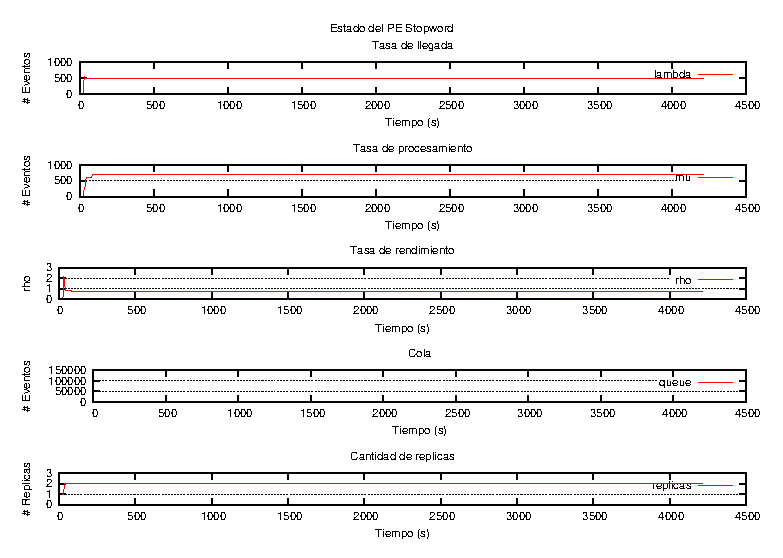
\includegraphics[scale=1.1]{images/exp/app1/uniform/cm/statusStopwordPE.eps}
    \caption{Estadísticas del PE Stopword en la primera aplicación con un envío constante de la fuente de datos con uso del monitor.}
    \label{fig:app1-uniform-statusStopwordPE-cm}
\end{figure}

\begin{figure}[p]
\centering
    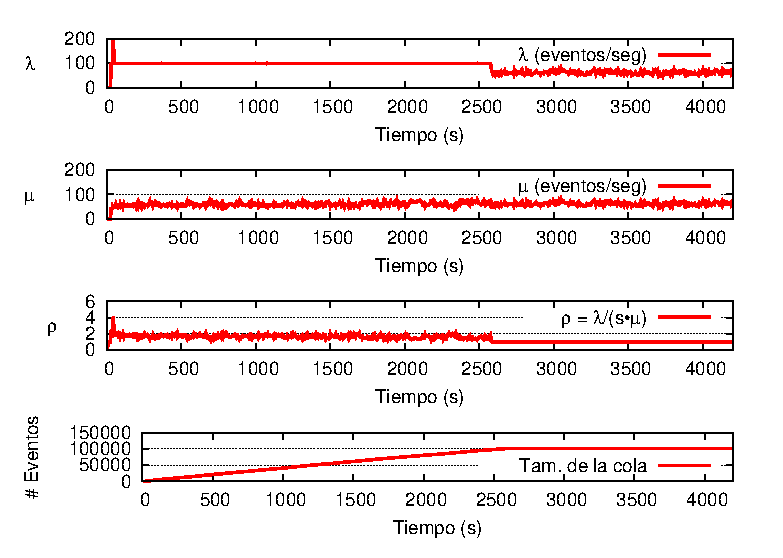
\includegraphics[scale=1.1]{images/exp/app1/uniform/sm/statusStopwordPE.eps}
    \caption{Estadísticas del PE Stopword en la primera aplicación con un envío constante de la fuente de datos sin uso del monitor.}
    \label{fig:app1-uniform-statusStopwordPE-sm}
\end{figure}

\begin{figure}[p]
\centering
    \includegraphics[scale=1.1]{images/exp/app1/uniform/cm/statusLanguagePE.eps}
    \caption{Estadísticas del PE Language en la primera aplicación con un envío constante de la fuente de datos con uso del monitor.}
    \label{fig:app1-uniform-statusLanguagePE-cm}
\end{figure}

\begin{figure}[p]
\centering
    \includegraphics[scale=1.1]{images/exp/app1/uniform/sm/statusLanguagePE.eps}
    \caption{Estadísticas del PE Language en la primera aplicación con un envío constante de la fuente de datos sin uso del monitor.}
    \label{fig:app1-uniform-statusLanguagePE-sm}
\end{figure}

\begin{figure}[p]
\centering
    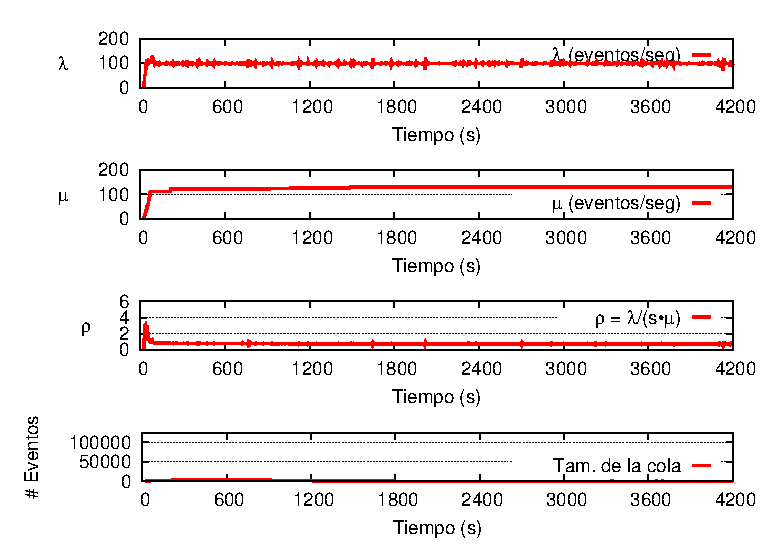
\includegraphics[scale=1.1]{images/exp/app1/uniform/cm/statusCounterPE.eps}
    \caption{Estadísticas del PE Counter en la primera aplicación con un envío constante de la fuente de datos con uso del monitor.}
    \label{fig:app1-uniform-statusCounterPE-cm}
\end{figure}

\begin{figure}[p]
\centering
    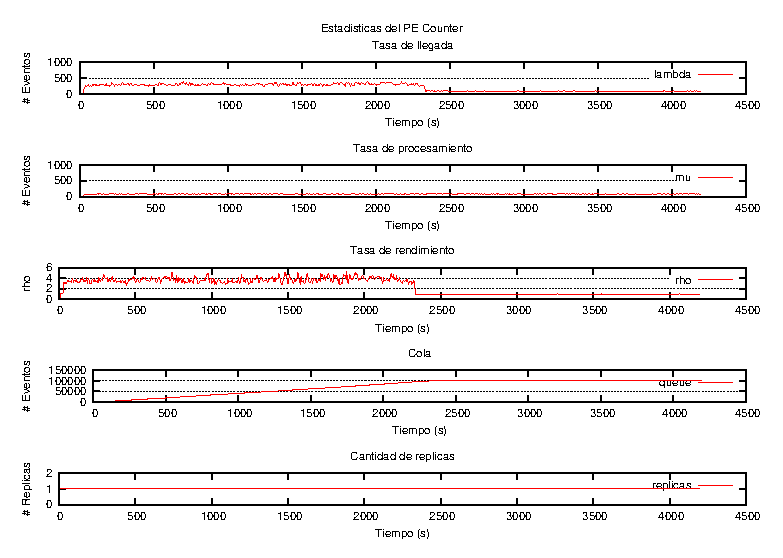
\includegraphics[scale=1.1]{images/exp/app1/uniform/sm/statusCounterPE.eps}
    \caption{Estadísticas del PE Counter en la primera aplicación con un envío constante de la fuente de datos sin uso del monitor.}
    \label{fig:app1-uniform-statusCounterPE-sm}
\end{figure}

\begin{figure}[p]
\centering
    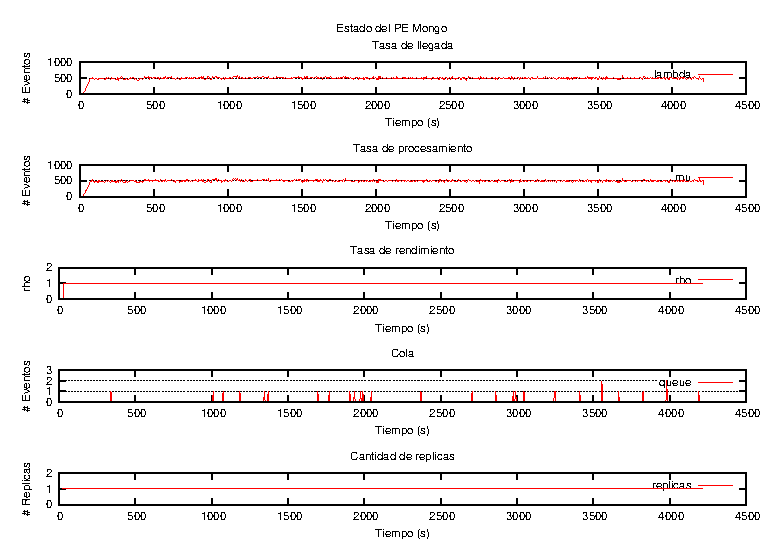
\includegraphics[scale=1.1]{images/exp/app1/uniform/cm/statusMongoPE.eps}
    \caption{Estadísticas del PE Mongo en la primera aplicación con un envío constante de la fuente de datos con uso del monitor.}
    \label{fig:app1-uniform-statusMongoPE-cm}
\end{figure}

\begin{figure}[p]
\centering
    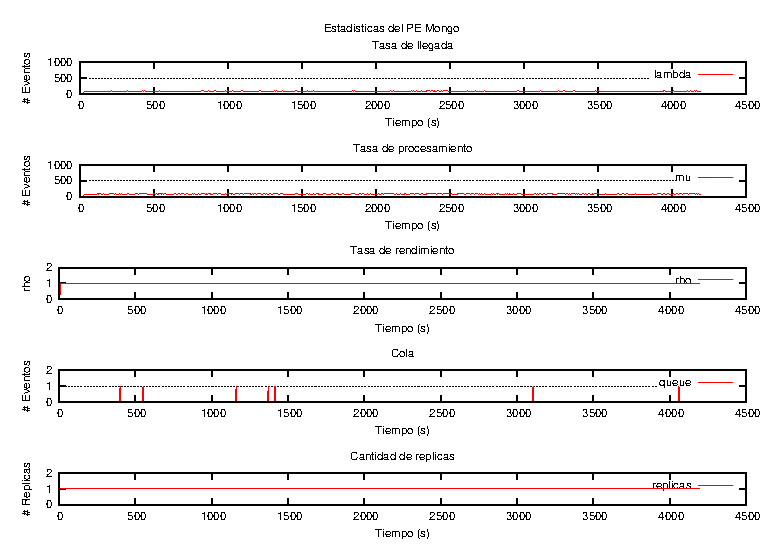
\includegraphics[scale=1.1]{images/exp/app1/uniform/sm/statusMongoPE.eps}
    \caption{Estadísticas del PE Mongo en la primera aplicación con un envío constante de la fuente de datos sin uso del monitor.}
    \label{fig:app1-uniform-statusMongoPE-sm}
\end{figure}

\begin{figure}[ht]
\centering

\begin{minipage}[c]{0.45\textwidth}
\centering
    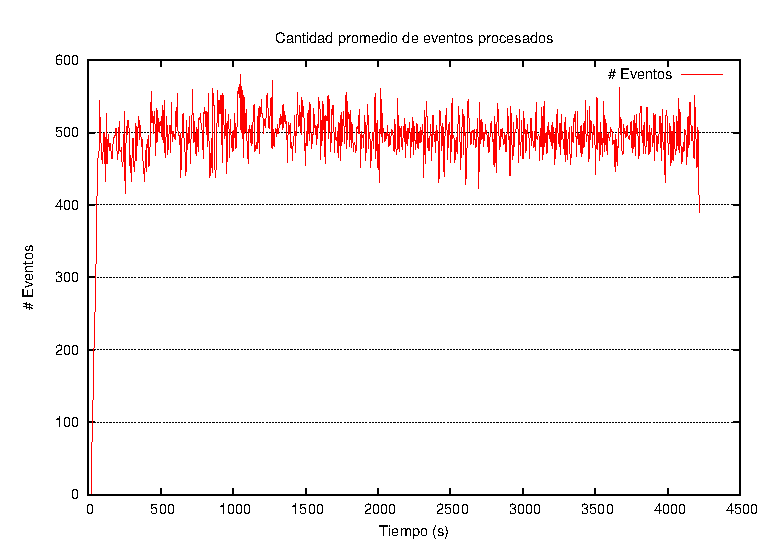
\includegraphics[width=\textwidth]{images/exp/app1/uniform/cm/avgEventProcess.eps}
    \caption{Tiempo promedio de procesamiento de un evento en la primera aplicación con una fuente de datos de distribución uniforme usando monitor.}
    \label{fig:app1-uniform-cm-avgEventProcess}
\end{minipage} \hspace*{1cm}
\begin{minipage}[c]{0.45\textwidth}
\centering
    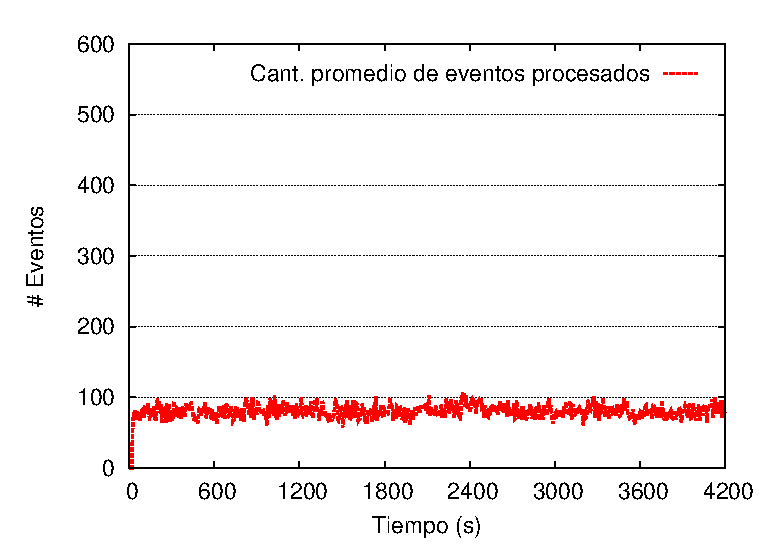
\includegraphics[width=\textwidth]{images/exp/app1/uniform/sm/avgEventProcess.eps}
    \caption{Tiempo promedio de procesamiento de un evento en la primera aplicación con una fuente de datos de distribución uniforme no usando monitor.}
    \label{fig:app1-uniform-sm-avgEventProcess}
\end{minipage}

\end{figure}

\begin{figure}[ht]
\centering

\begin{minipage}[c]{0.45\textwidth}
\centering
    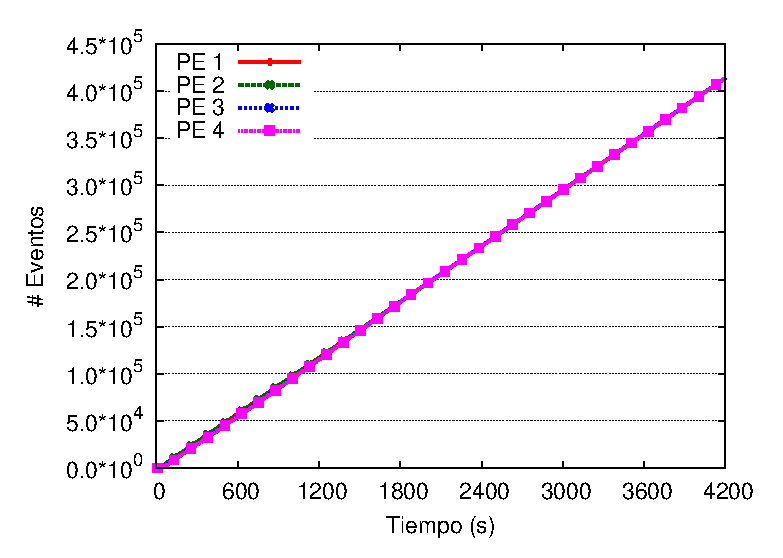
\includegraphics[width=\textwidth]{images/exp/app1/uniform/cm/eventCount.eps}
    \caption{Cantidad total de eventos procesados en la primera aplicación con una fuente de datos de distribución uniforme usando monitor.}
    \label{fig:app1-uniform-eventCount-cm}
\end{minipage} \hspace*{1cm}
\begin{minipage}[c]{0.45\textwidth}
\centering
    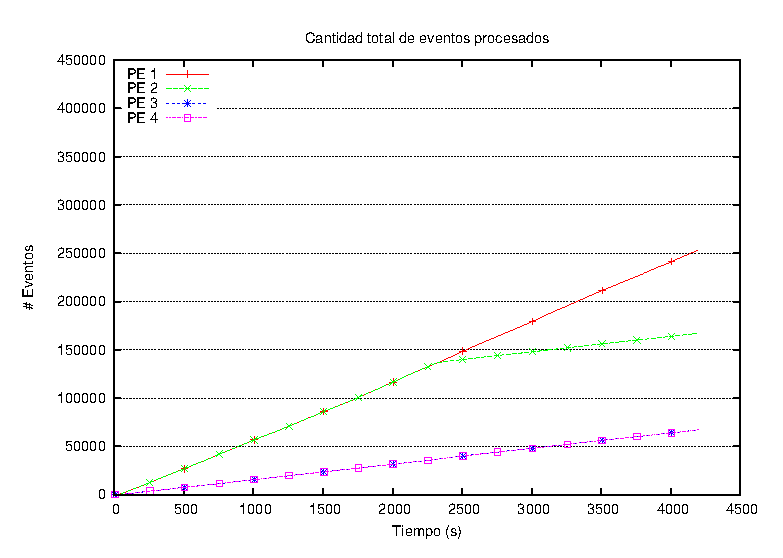
\includegraphics[width=\textwidth]{images/exp/app1/uniform/sm/eventCount.eps}
    \caption{Cantidad total de eventos procesados en la primera aplicación con una fuente de datos de distribución uniforme no usando monitor.}
    \label{fig:app1-uniform-eventCount-sm}
\end{minipage}

\end{figure}

El segundo experimento consistió en enviar un flujo dinámico de datos, y realizando una comparación de los sistemas con y sin monitoreo de la carga de los operadores.

En construcción...

%Para analizar el comportamiento del sistema, se puede observar en la Figura \ref{fig:app1-normal-statusStopwordPE-cm} y \ref{fig:app1-normal-statusStopwordPE-sm} las estadísticas del primer operador del grafo, con y sin monitoreo en la carga de los operadores respectivamente. La tasa de llegada ($\lambda$) se puede observar como en el primer gráfico es dinámica, pero no así en el segundo gráfico, debido que en el segundo 2600 surge una disminución del flujo de datos. Esto se debe a la acumulación de eventos en el \textit{buffer}, por lo que se genera cola en el PE, lo cual impide almacenar mayor cantidad de eventos, dado que la cantidad de eventos que se procesan es menor que la cantidad de eventos que llegan.

%Por otra parte, la tasa de rendimiento de la Figura \ref{fig:app1-normal-statusStopwordPE-cm} se estabiliza dentro de los primeros 100 segundos, debido que el sistema de distribución de carga detectó una sobrecarga en el operador y replicó el operador, a diferencia de la Figura \ref{fig:app1-normal-statusStopwordPE-sm}, en el cual el operador posee una tasa de rendimiento estable que bordea entre 1 y 2, hasta el segundo 2600, donde disminuye debido que la tasa de llegada es menor.

%En la Figura \ref{fig:app1-normal-statusLanguagePE-cm} y \ref{fig:app1-normal-statusLanguagePE-sm} se puede ver el siguiente operador del gráfico, el cual no tiene mayor inconveniente, a excepción del segundo 2400, donde el sin monitoreo disminuye considerablemente la tasa de procesamiento del PE. Si analizamos la Figura \ref{fig:app1-normal-statusStopwordPE-sm} y \ref{fig:app1-normal-statusLanguagePE-sm}, empiezan aproximadamente desde el rango de tiempo (2400s,2600s) los problemas de procesamiento de los operadores, por lo tanto, se puede deducir que si el problema surge en un operador no es un problema aislado, sino que también influye a los siguientes operadores.

%Por otra parte, en la Figura \ref{fig:app1-normal-statusCounterPE-cm}, se puede observar como con el transcurs de los primeros 100 segundos fue aumentando la cantidad de réplicas hasta llegar a 5, el cual fue su óptimo, para ir procesando la cantidad de eventos y disminuir la cola existente en el sistema. Esto en contra posición a la Figura \ref{fig:app1-normal-statusCounterPE-sm}, donde la inexistencia de replicación, genera una cola la cual se mantiene constante en el segundo 2400. Esto se debe a que la cantidad de eventos almacenados en el \textit{buffer} está lleno, por lo que no pueden agregarse más eventos y bloqueando el \textit{buffer}.

%Finalmente, se encuentra el último operador, el cual no presenta grandes inconvenientes tanto en la Figura \ref{fig:app1-normal-statusMongoPE-cm} y \ref{fig:app1-normal-statusMongoPE-sm}, esto debido que el tiempo de procesamiento es bajo, y nunca llega una cantidad de eventos considerable para existir una sobrecarga en éste. Además es importante destacar que en la Figura \ref{fig:app1-normal-statusMongoPE-sm} llega una menor tasa de llegada, exactamente un $83,827\%$ menos de eventos que un SPS ejecutado con el sistema de distribución de carga.

%Por otra parte, también se analizó la cantidad promedio de eventos procesados en cada período, la cual está graficada en la Figura \ref{fig:app1-normal-avgEventProcess}. Como se puede apreciar, en los primeros 50 segundos se puede ver una mejora considerable en la cantidad de eventos procesados, donde posteriormente se procesan aproximadamente 480 eventos por período con monitoreo, a diferencia del SPS sin monitoreo, que procesa 90 eventos por período aproximadamente, habiendo una mejora del $615,38\%$. Esta mejora se debe al factor de la replicación de los operadores que posee mayor sobrecarga, por lo que al aumentar la cantidad de réplicas, aumenta la tasa de procesamiento, lo significa mayor cantidad de flujo para el próximo operador.

%Así también, se puede observar en la Figura \ref{fig:app1-normal-eventCount-cm} y \ref{fig:app1-normal-eventCount-sm} la cantidad total de eventos procesados con el transcurso de la ejecución en cada uno de los operadores, con y sin uso del monitoreo respectivamente. En el primer gráfico se denota como los cuatro operadores del SPS van aumentando casi linealmente de la misma manera, tan sólo existe una menor cantidad de eventos procesados en el tercer PE, lo cual se traslada al cuatro PE, debido que al procesar menor cantidad de eventos el tercer PE, llega menor cantidad de datos al cuarto PE. En este gráfico se llegó a un total de 401.618 eventos procesados. En cambio, en el segundo gráfico existe una curva muy distinta por los distintos operadores, lo cual se ve reflejado desde la cantidad de eventos procesados en el primer operador hasta la cantidad total de eventos procesados por el sistema, el cual es de 67.141, existiendo una mejora del $598,171\%$ con el uso del sistema de distribución de carga.

%\begin{figure}[p]
%\centering
%    \includegraphics[scale=1.1.1]{images/exp/app1/normal/cm/statusStopwordPE.eps}
%    \caption{Estadísticas del PE Stopword en la primera aplicación con un envío constante de la fuente de datos con uso del monitor.}
%    \label{fig:app1-uniform-statusStopwordPE-cm}
%\end{figure}
%
%\begin{figure}[p]
%\centering
%    \includegraphics[scale=1.1.1]{images/exp/app1/normal/sm/statusStopwordPE.eps}
%    \caption{Estadísticas del PE Stopword en la primera aplicación con un envío constante de la fuente de datos sin uso del monitor.}
%    \label{fig:app1-uniform-statusStopwordPE-sm}
%\end{figure}
%
%\begin{figure}[p]
%\centering
%    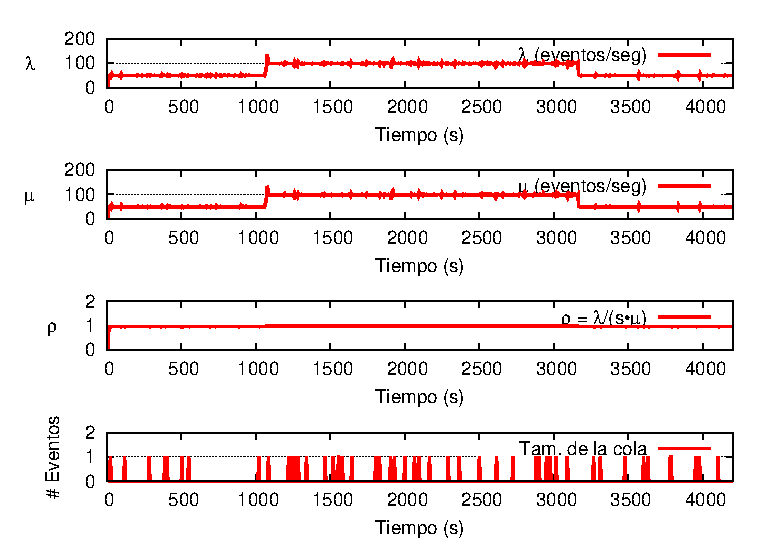
\includegraphics[scale=1.1]{images/exp/app1/normal/cm/statusLanguagePE.eps}
%    \caption{Estadísticas del PE Language en la primera aplicación con un envío constante de la fuente de datos con uso del monitor.}
%    \label{fig:app1-uniform-statusLanguagePE-cm}
%\end{figure}
%
%\begin{figure}[p]
%\centering
%    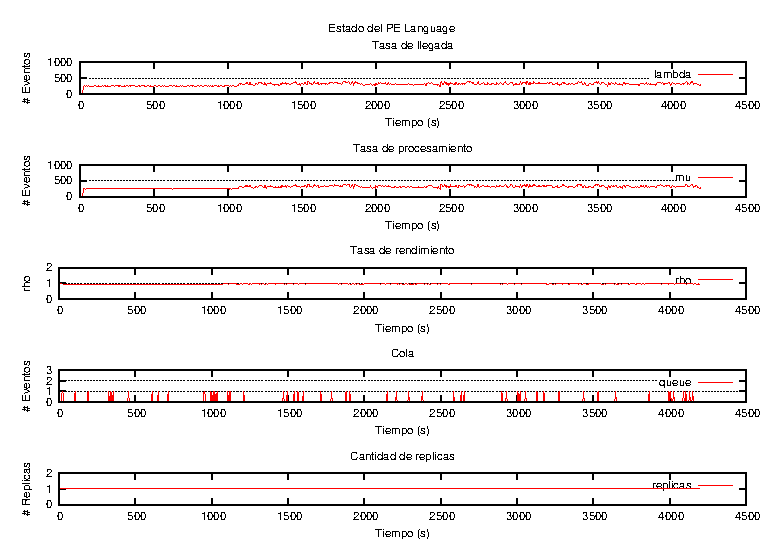
\includegraphics[scale=1.1]{images/exp/app1/normal/sm/statusLanguagePE.eps}
%    \caption{Estadísticas del PE Language en la primera aplicación con un envío constante de la fuente de datos sin uso del monitor.}
%    \label{fig:app1-uniform-statusLanguagePE-sm}
%\end{figure}
%
%\begin{figure}[p]
%\centering
%    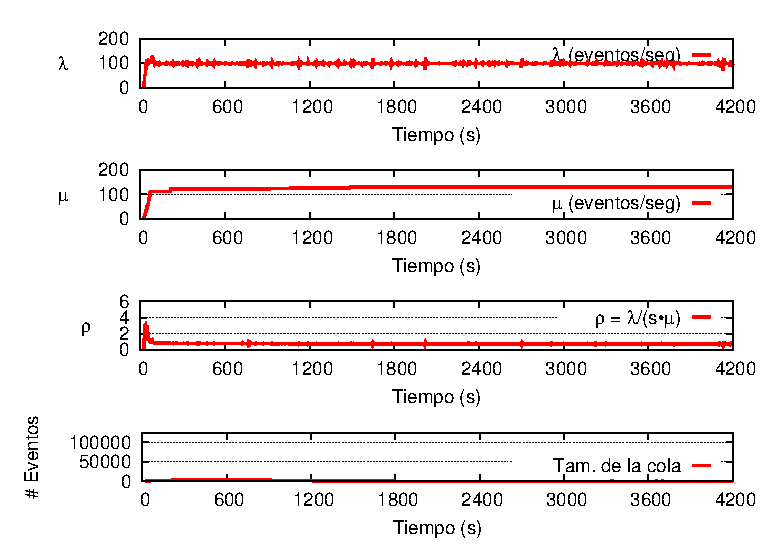
\includegraphics[scale=1.1]{images/exp/app1/uniform/cm/statusCounterPE.eps}
%    \caption{Estadísticas del PE Counter en la primera aplicación con un envío constante de la fuente de datos con uso del monitor.}
%    \label{fig:app1-uniform-statusCounterPE-cm}
%\end{figure}
%
%\begin{figure}[p]
%\centering
%    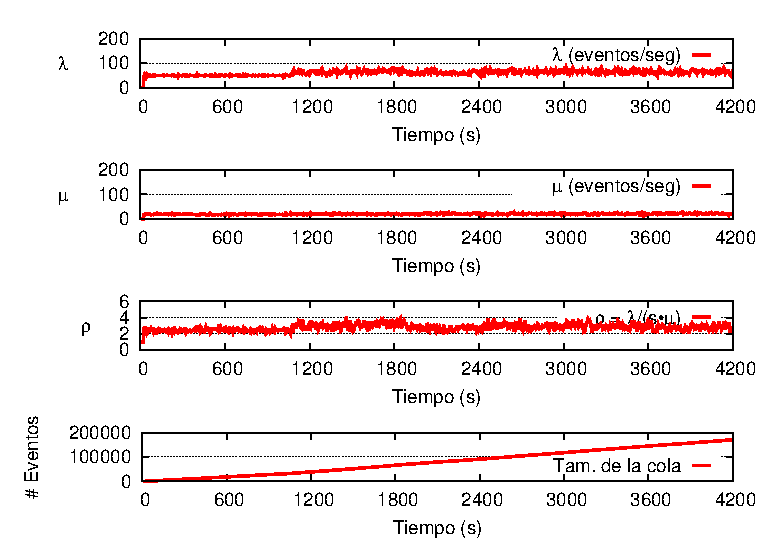
\includegraphics[scale=1.1]{images/exp/app1/normal/sm/statusCounterPE.eps}
%    \caption{Estadísticas del PE Counter en la primera aplicación con un envío constante de la fuente de datos sin uso del monitor.}
%    \label{fig:app1-uniform-statusCounterPE-sm}
%\end{figure}
%
%\begin{figure}[p]
%\centering
%    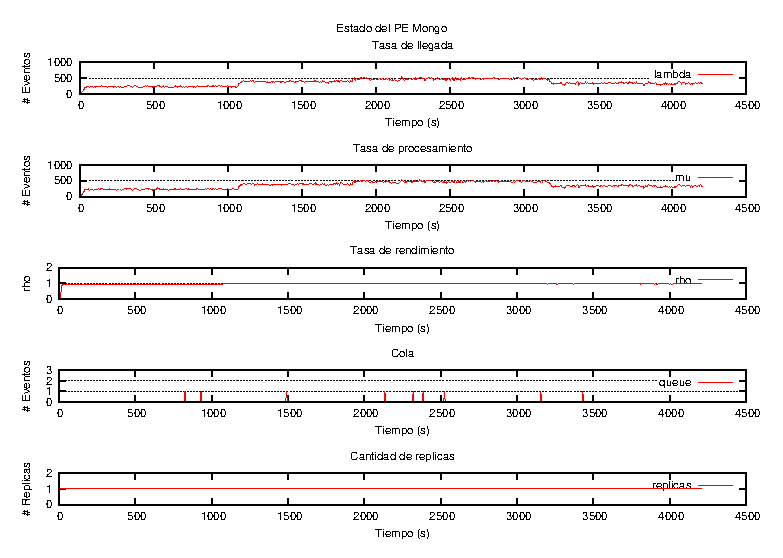
\includegraphics[scale=1.1]{images/exp/app1/normal/cm/statusMongoPE.eps}
%    \caption{Estadísticas del PE Mongo en la primera aplicación con un envío constante de la fuente de datos con uso del monitor.}
%    \label{fig:app1-uniform-statusMongoPE-cm}
%\end{figure}
%
%\begin{figure}[p]
%\centering
%    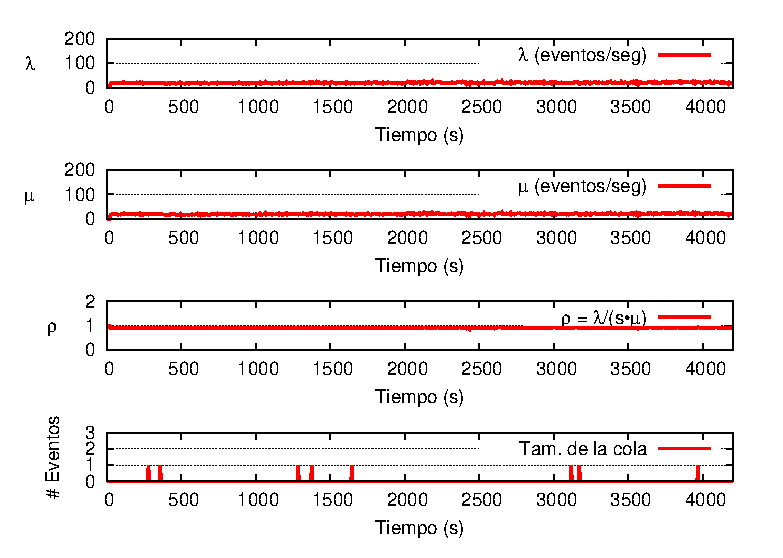
\includegraphics[scale=1.1]{images/exp/app1/normal/sm/statusMongoPE.eps}
%    \caption{Estadísticas del PE Mongo en la primera aplicación con un envío constante de la fuente de datos sin uso del monitor.}
%    \label{fig:app1-uniform-statusMongoPE-sm}
%\end{figure}
%
%\begin{figure}[ht]
%\centering
%
%\begin{minipage}[c]{0.45\textwidth}
%\centering
%    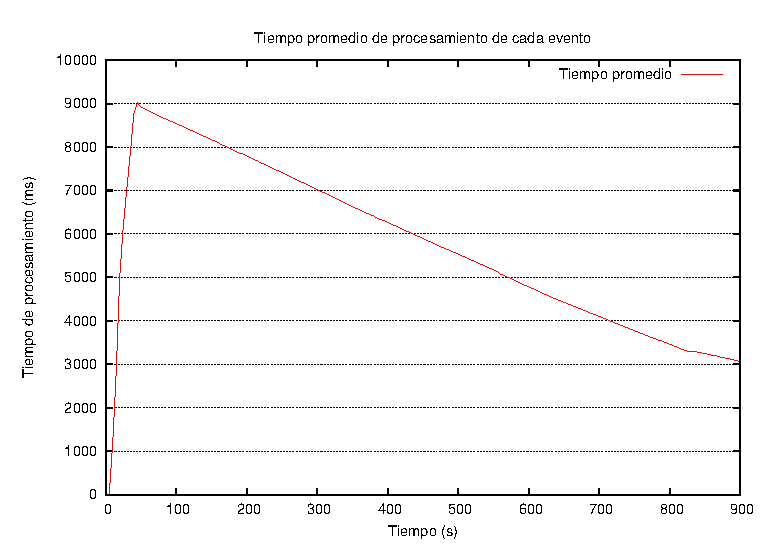
\includegraphics[width=\textwidth]{images/exp/app1/normal/avgTimeTotal.eps}
%    \caption{Tiempo promedio de procesamiento de un evento en la primera aplicación con una fuente de datos de distribución uniforme.}
%    \label{fig:app1-uniform-avgTimeTotal}
%\end{minipage} \hspace*{1cm}
%\begin{minipage}[c]{0.45\textwidth}
%\centering
%    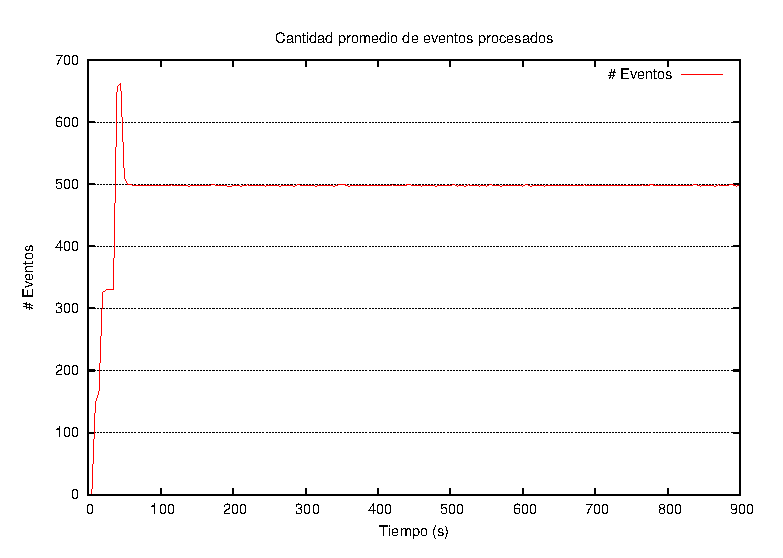
\includegraphics[width=\textwidth]{images/exp/app1/normal/avgEventProcess.eps}
%    \caption{Cantidad promedio de eventos procesados en un período de tiempo en la primera aplicación con una fuente de datos de distribución uniforme.}
%    \label{fig:app1-uniform-avgEventProcess}
%\end{minipage}
%
%\end{figure}
%
%\begin{figure}[ht]
%\centering
%
%\begin{minipage}[c]{0.45\textwidth}
%\centering
%    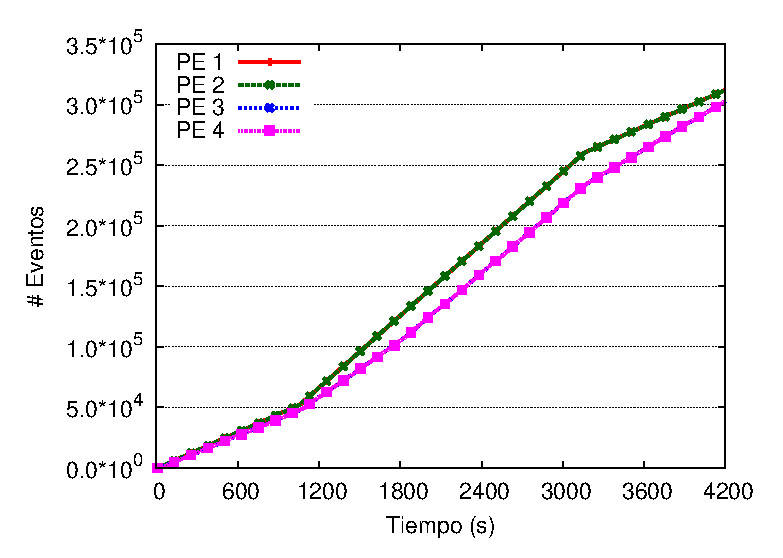
\includegraphics[width=\textwidth]{images/exp/app1/normal/cm/eventCount.eps}
%    \caption{Cantidad total de eventos procesados en la primera aplicación con una fuente de datos de distribución uniforme usando monitor.}
%    \label{fig:app1-uniform-eventCount-cm}
%\end{minipage} \hspace*{1cm}
%\begin{minipage}[c]{0.45\textwidth}
%\centering
%    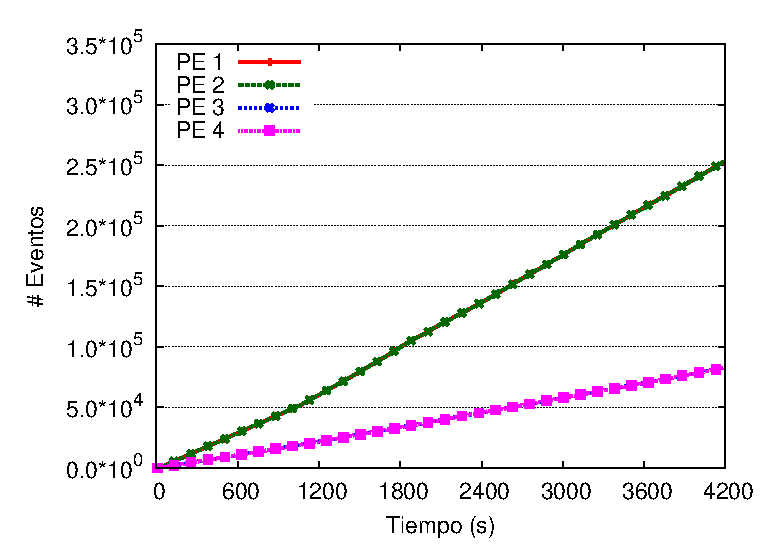
\includegraphics[width=\textwidth]{images/exp/app1/normal/sm/eventCount.eps}
%    \caption{Cantidad total de eventos procesados en la primera aplicación con una fuente de datos de distribución uniforme no usando monitor.}
%    \label{fig:app1-uniform-eventCount-sm}
%\end{minipage}
%
%\end{figure}

\subsection{Segundo experimento}
En la segunda aplicación se procedió a realizar cuatro experimentos distintos, donde cada par era una comparación del experimento con y sin uso del monitor. Las dos primeras se consideró un envío constante de la fuente de datos, y las dos segundas se consideró un envío dinámico de la fuente de datos.

Para el análisis de los experimento se consideró la cantidad total de eventos y las estadísticas de cada PE en el transcurso de la ejecución de la aplicación.

Para analizar el comportamiento del sistema, se puede observar en la Figura \ref{fig:app2-uniform-statusSplitPE-cm} y \ref{fig:app2-uniform-statusSplitPE-sm} las estadísticas del primer operador del grafo, con y sin monitoreo en la carga de los operadores respectivamente. En el primer gráfico la tasa de llegada ($\lambda$) en los primeros 200 segundos se encuentran ciertos \textit{peak}, los cuales se deben al \textit{delay} en la toma de estadísticas, producto de la replicación del siguiente PE en el sistema, como se puede demostrar en la Figura \ref{fig:app2-uniform-statusCounterPE-cm}. Independiente del uso del monitoreo, se puede denotar que el comportamiento entre los dos PEs es prácticamente igual, y esto se debe a que la carga que posee este PE es casi nula, debido que es un PE auxiliar para el PE Counter, dado que sólo separa la cantidad de palabras para que el PE Counter cuente la frecuencia de cada palabra en la información entrante.

En cambio, en la Figura \ref{fig:app2-uniform-statusCounterPE-cm} y \ref{fig:app2-uniform-statusCounterPE-sm} se puede observar una diferencia en los rendimientos del PE. Esto se debe, a que este operador posee una carga una alta carga, dado que posee una gran bolsa de palabras para comparar con las palabras del \textit{tweets}. Debido a esto, al generar las réplicas, se produce una mejora considerable del operador en los primeros 100 segundo.

En este caso, el predictor se activó, dado que se realiza un aumento de 9 a 14 réplicas. Si bien, la cantidad de réplicas fue mayor a lo necesario, dado que el promedio de tasa de procesamiento posterior al segundo 100 es de 0.63, no se considera el operador en estado ocioso, por lo que no se disminuye la cantidad de réplicas.

Un detalle importante a destacar, es que independiente que se generen más réplicas, el sistema no procesa mayor cantidad de eventos, como se puede observar en la cola del operador. Este problema fue detectado por la implementanción realizada en el SPS de S4, dado que posterior a un período de tiempo, la tasa de procesamiento disminuye considerablemente. La hipótesis que se posee de este problema es que el sistema no elimina los eventos procesados, por lo que independiente de si es procesado o no, continúa en el \textit{buffer}, de esta manera, la cola sigue aumentando, sin ser removido por el \textit{garbage collector} de Java.

En el último PE, se puede ver que existe una baja cantidad de eventos entrantes, como se muestra en la Figura \ref{fig:app2-uniform-statusMergePE-cm} y \ref{fig:app2-uniform-statusMergePE-sm}. Esto se debe, a que los eventos entrantes sólo son enviados cada 10 segundos por el PE Counter, por lo que son una pequeña cantidad de eventos los que son enviados. En el primer gráfico, se puede ver que la tasa de llegada aumenta posterior a los 100 segundos, esto se debe a que se realizaron réplicas, por lo que cada una de las réplicas envía un evento cada 10 segundos, habiendo mayor flujo. En cambio, en el segundo gráfico, el flujo de entrada sólo se condiciona por una réplica, por lo que no se procesa la misma cantidad de eventos. Cabe destacar, que como la tasa de llegada es pequeña, no existe un problema en la tasa de rendimiento del operador, aunque posea un alto cómputo de ejecución su tarea.

Finalmente, en la Figura \ref{fig:app2-uniform-eventCount-cm} y \ref{fig:app2-uniform-eventCount-sm} se muestra la cantidad total de eventos procesados. En el primer gráfico se puede analizar que la diferencia de la pendiente entre las rectas del primer y segundo PE, es menor que en el segundo gráfico. Esto se debe al aumento de la cantidad de réplicas, de esta manera puede procesar mayor cantidad de eventos, siendo un procesamiento de 181114 con uso el monitor contra 30049 sin uso del monitor, habiendo una mejora del $602,7288\%$. El tercer PE procesa pocos eventos, debido que sólo le llega un evento por réplica cada 10 segundos.

Dentro de los análisis importantes a realizar por parte de este experimento, es que en el gráfico \ref{fig:app1-uniform-eventCount-cm} no existe una mejora por parte del segundo PE de manera paralela al flujo de datos emanado por el primer PE. Esto se debió al funcionamiento de la herramienta S4, debido que después de un período de tiempo no procesa la misma cantidad de eventos, por lo que independiente que se siga replicando, no existe una mejora en el sistema. Este problema se debe a la forma en que esta implementando el \textit{buffer} de S4, debido que éste se va llenando, pero no se libera, por lo que al llenarse bloquea el envió de los datos por parte del sistema, generando una demora en el procesamiento.

\begin{figure}[p]
\centering
    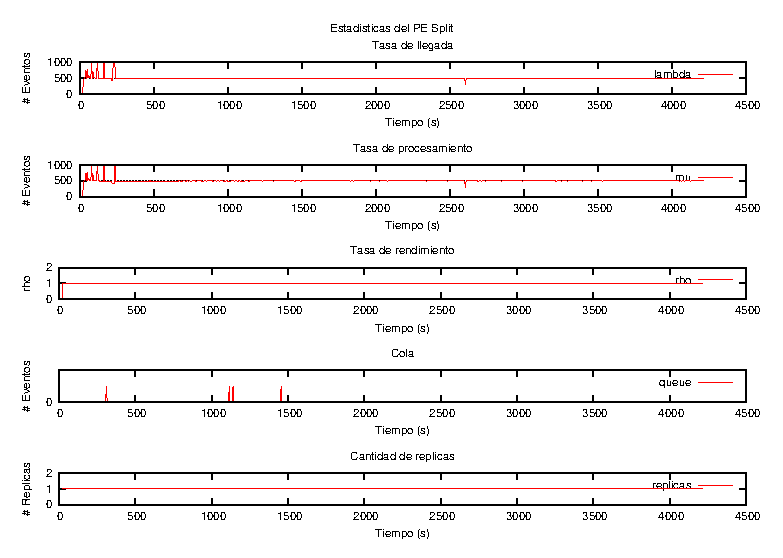
\includegraphics[scale=1.1]{images/exp/app2/uniform/cm/statusSplitPE.eps}
    \caption{Estadísticas del PE Mongo en la primera aplicación con un envío constante de la fuente de datos con uso del monitor.}
    \label{fig:app2-uniform-statusSplitPE-cm}
\end{figure}

\begin{figure}[p]
\centering
    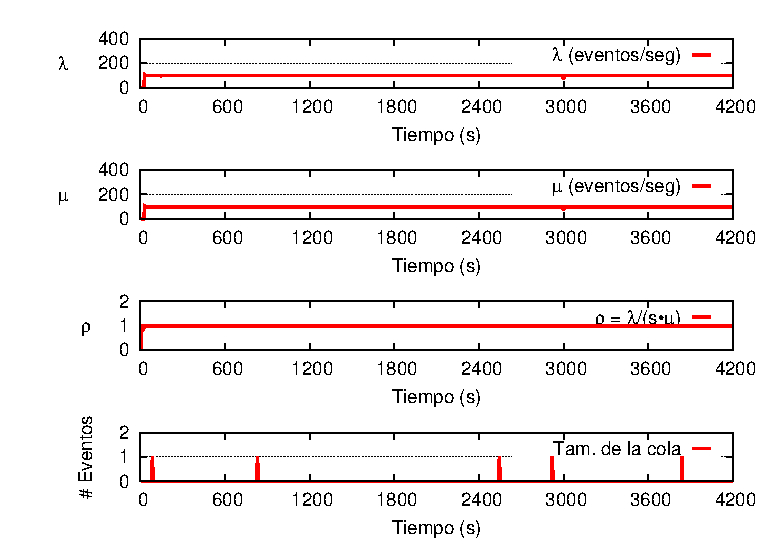
\includegraphics[scale=1.1]{images/exp/app2/uniform/sm/statusSplitPE.eps}
    \caption{Estadísticas del PE Mongo en la primera aplicación con un envío constante de la fuente de datos sin uso del monitor.}
    \label{fig:app2-uniform-statusSplitPE-sm}
\end{figure}

\begin{figure}[p]
\centering
    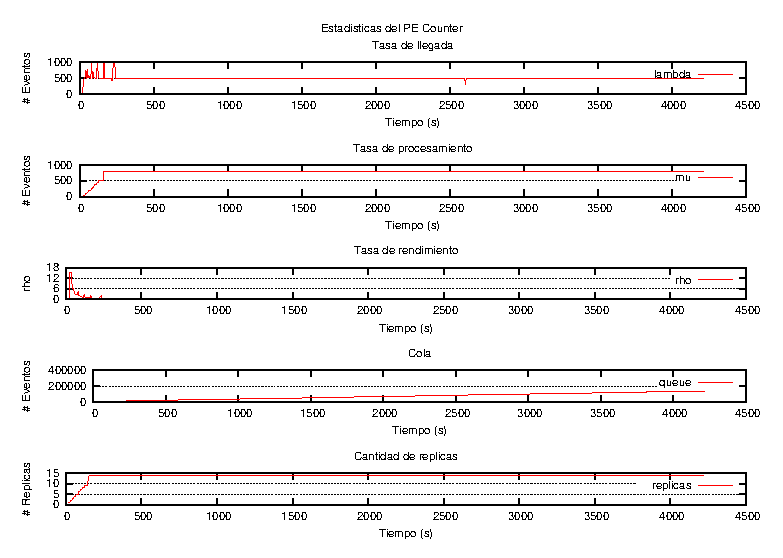
\includegraphics[scale=1.1]{images/exp/app2/uniform/cm/statusCounterPE.eps}
    \caption{Estadísticas del PE Mongo en la primera aplicación con un envío constante de la fuente de datos con uso del monitor.}
    \label{fig:app2-uniform-statusCounterPE-cm}
\end{figure}

\begin{figure}[p]
\centering
    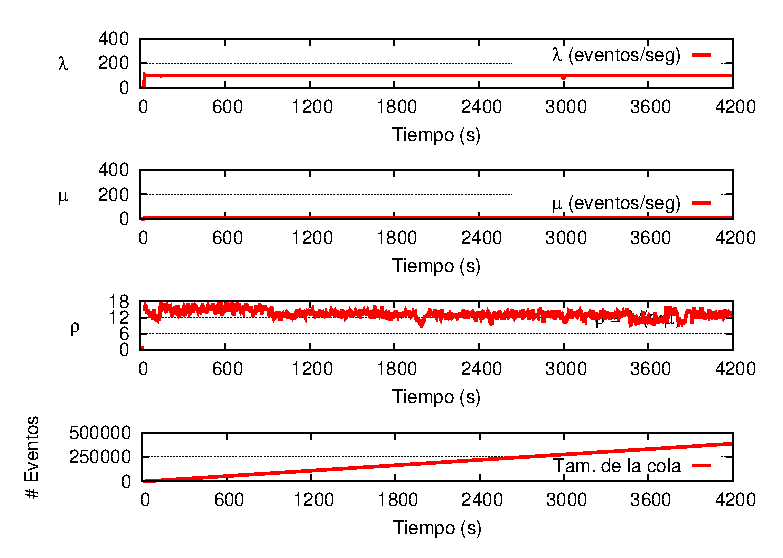
\includegraphics[scale=1.1]{images/exp/app2/uniform/sm/statusCounterPE.eps}
    \caption{Estadísticas del PE Mongo en la primera aplicación con un envío constante de la fuente de datos sin uso del monitor.}
    \label{fig:app2-uniform-statusCounterPE-sm}
\end{figure}

\begin{figure}[p]
\centering
    \includegraphics[scale=1.1]{images/exp/app2/uniform/cm/statusMergePE.eps}
    \caption{Estadísticas del PE Mongo en la primera aplicación con un envío constante de la fuente de datos con uso del monitor.}
    \label{fig:app2-uniform-statusMergePE-cm}
\end{figure}

\begin{figure}[p]
\centering
    \includegraphics[scale=1.1]{images/exp/app2/uniform/sm/statusMergePE.eps}
    \caption{Estadísticas del PE Mongo en la primera aplicación con un envío constante de la fuente de datos sin uso del monitor.}
    \label{fig:app2-uniform-statusMergePE-sm}
\end{figure}

\begin{figure}[ht]
\centering

\begin{minipage}[c]{0.45\textwidth}
\centering
    \includegraphics[width=\textwidth]{images/exp/app2/uniform/cm/eventCount.eps}
    \caption{Cantidad total de eventos procesados en la primera aplicación con una fuente de datos de distribución uniforme usando monitor.}
    \label{fig:app2-uniform-eventCount-cm}
\end{minipage} \hspace*{1cm}
\begin{minipage}[c]{0.45\textwidth}
\centering
    \includegraphics[width=\textwidth]{images/exp/app2/uniform/sm/eventCount.eps}
    \caption{Cantidad total de eventos procesados en la primera aplicación con una fuente de datos de distribución uniforme no usando monitor.}
    \label{fig:app2-uniform-eventCount-sm}
\end{minipage}

\end{figure}

\subsection{Tercer experimento}
En la tercera aplicación se procedió a realizar dos experimentos, ambos con envío constante de la fuente de datos, donde el SPS funciona con y sin uso del monitor.

Para el análisis de los experimento se consideró el consumo de RAM, el uso de la CPU, la cantidad total de eventos, la cantidad promedio de eventos procesados por período y las estadísticas de cada PE en el transcurso de la ejecución de la aplicación.

\begin{figure}[p]
\centering
    \includegraphics[scale=1.1]{images/exp/app1/uniform/cm/statusStopwordPE.eps}
    \caption{Estadísticas del PE Stopword en la primera aplicación con un envío constante de la fuente de datos con uso del monitor.}
    \label{fig:app1-uniform-statusStopwordPE-cm}
\end{figure}

\begin{figure}[p]
\centering
    \includegraphics[scale=1.1]{images/exp/app1/uniform/sm/statusStopwordPE.eps}
    \caption{Estadísticas del PE Stopword en la primera aplicación con un envío constante de la fuente de datos sin uso del monitor.}
    \label{fig:app1-uniform-statusStopwordPE-sm}
\end{figure}

\begin{figure}[p]
\centering
    \includegraphics[scale=1.1]{images/exp/app1/uniform/cm/statusLanguagePE.eps}
    \caption{Estadísticas del PE Language en la primera aplicación con un envío constante de la fuente de datos con uso del monitor.}
    \label{fig:app1-uniform-statusLanguagePE-cm}
\end{figure}

\begin{figure}[p]
\centering
    \includegraphics[scale=1.1]{images/exp/app1/uniform/sm/statusLanguagePE.eps}
    \caption{Estadísticas del PE Language en la primera aplicación con un envío constante de la fuente de datos sin uso del monitor.}
    \label{fig:app1-uniform-statusLanguagePE-sm}
\end{figure}

\begin{figure}[p]
\centering
    \includegraphics[scale=1.1]{images/exp/app1/uniform/cm/statusCounterPE.eps}
    \caption{Estadísticas del PE Counter en la primera aplicación con un envío constante de la fuente de datos con uso del monitor.}
    \label{fig:app1-uniform-statusCounterPE-cm}
\end{figure}

\begin{figure}[p]
\centering
    \includegraphics[scale=1.1]{images/exp/app1/uniform/sm/statusCounterPE.eps}
    \caption{Estadísticas del PE Counter en la primera aplicación con un envío constante de la fuente de datos sin uso del monitor.}
    \label{fig:app1-uniform-statusCounterPE-sm}
\end{figure}

\begin{figure}[p]
\centering
    \includegraphics[scale=1.1]{images/exp/app1/uniform/cm/statusMongoPE.eps}
    \caption{Estadísticas del PE Mongo en la primera aplicación con un envío constante de la fuente de datos con uso del monitor.}
    \label{fig:app1-uniform-statusMongoPE-cm}
\end{figure}

\begin{figure}[p]
\centering
    \includegraphics[scale=1.1]{images/exp/app1/uniform/sm/statusMongoPE.eps}
    \caption{Estadísticas del PE Mongo en la primera aplicación con un envío constante de la fuente de datos sin uso del monitor.}
    \label{fig:app1-uniform-statusMongoPE-sm}
\end{figure}

\begin{figure}[ht]
\centering

\begin{minipage}[c]{0.45\textwidth}
\centering
    \includegraphics[width=\textwidth]{images/exp/app1/uniform/cm/avgEventProcess.eps}
    \caption{Tiempo promedio de procesamiento de un evento en la primera aplicación con una fuente de datos de distribución uniforme usando monitor.}
    \label{fig:app1-uniform-cm-avgEventProcess}
\end{minipage} \hspace*{1cm}
\begin{minipage}[c]{0.45\textwidth}
\centering
    \includegraphics[width=\textwidth]{images/exp/app1/uniform/sm/avgEventProcess.eps}
    \caption{Tiempo promedio de procesamiento de un evento en la primera aplicación con una fuente de datos de distribución uniforme no usando monitor.}
    \label{fig:app1-uniform-sm-avgEventProcess}
\end{minipage}

\end{figure}

\begin{figure}[ht]
\centering

\begin{minipage}[c]{0.45\textwidth}
\centering
    \includegraphics[width=\textwidth]{images/exp/app1/uniform/cm/eventCount.eps}
    \caption{Cantidad total de eventos procesados en la primera aplicación con una fuente de datos de distribución uniforme usando monitor.}
    \label{fig:app1-uniform-eventCount-cm}
\end{minipage} \hspace*{1cm}
\begin{minipage}[c]{0.45\textwidth}
\centering
    \includegraphics[width=\textwidth]{images/exp/app1/uniform/sm/eventCount.eps}
    \caption{Cantidad total de eventos procesados en la primera aplicación con una fuente de datos de distribución uniforme no usando monitor.}
    \label{fig:app1-uniform-eventCount-sm}
\end{minipage}

\end{figure}
\chapter{Conclusiones}
\label{cap:conclusiones}
En este trabajo se ha propuesto la generación de un sistema elástico, cuyo objetivo es lograr una mejor utilización de los recursos disponibles \hl{en un sistema} y con ello un aumento en su capacidad de procesamiento y escalabilidad.

\section{Detalles de la contribución}
Dentro de las contribuciones de este trabajo se encuentra el diseño e implementación de un modelo elástico que es capaz de lidiar con el dinamismo del flujo de eventos o tráfico de datos. En este modelo se diseñaron cuatro módulos, los cuales estaban compuestos por un módulo de monitoreo, que recolecta las estadísticas, un módulo reactivo y predictivo, que estima la carga de cada operador en el presente y a futuro respectivamente, y un módulo de administración de réplicas, que aumenta o disminuye el número de réplicas de un operador según la carga de éste.

El módulo reactivo que se ha diseñado e implementado tiene como función analizar la carga actual del operador, cumpliendo así el primer objetivo de este trabajo, el cual consiste en dise\~nar e implementar un algoritmo reactivo que permita analizar en el momento la carga de los operadores.

Por otra parte, se ha diseñado e implementando el módulo predictivo, cuya función es estimar la carga de un operador en una ventana de tiempo futura, cumpliendo el segundo objetivo, el cual consiste en dise\~nar e implementar un algoritmo de predicci\'on que permita estimar la carga de los operadores.

Así mismo, se ha diseñado e implementado un módulo de administración de réplicas, el cual se encarga de administrar la cantidad de réplicas de los operadores del SPS de forma elástica, vale decir, que aumenta o disminuye el número de réplicas acorde al tráfico recibido.

%Por otra parte, se han diseñado y construido distintos experimentos que permita validar la hipótesis planteada, cuyo planteamiento es la utilización de modelo elástico de tal manera que mejore el rendimiento del SPS y se procese mayor cantidad de eventos, cumpliendo así el cuarto objetivo planteado.

Para validar el modelo elástico se \hl{han} construido tres escenarios para la experimentación, donde el \hl{primero} consiste en una aplicación que realiza operaciones sin estados, la segunda una aplicación que realiza operaciones con estados, y la tercera una aplicación sintética. De esta manera, el objetivo es evaluar el rendimiento del sistema utilizando el modelo elástico.

%Y finalmente, se ha evaluado y analizado el rendimiento del sistema a través de distintas aplicaciones generadas sobre un SPS, en este caso sobre S4. En todas las aplicaciones ha mejorado la cantidad de eventos procesados, dependiendo del tipo de aplicación se ha detectado un aumento de hasta 8 veces más eventos procesados. Como se había mencionado anterior, al posee mayor cantidad de datos procesados, se posee mayor precisión en la información obtenida. Por otra parte, el costo asociado por la implementación del modelo elástico es de un aumento de $0,0119\%$, pero con una disminución del uso de la memoria RAM, la cual es de un $1,5187\%$, lo cual significa que el sistema si bien puede aumentar el consumo de CPU, disminuye el uso de la RAM.

Haciendo uso de los escenarios, se ha evaluado y analizado el rendimiento del sistema con y sin uso del modelo elástico. Los resultados muestran que para todos los escenarios se ha mejorado la cantidad de eventos procesados. Dependiendo del tipo de escenario, se ha detectado un aumento de hasta 9 veces en el \textit{throughput} de la aplicación. Este es un resultado importante, puesto que al poseer una mayor cantidad de datos procesados, se puede lograr una mayor precisión en la información obtenida. Por otra parte, el costo asociado a la implementación del modelo elástico en relación a la CPU es de un aumento del $0,01\%$, sin embargo la memoria RAM utilizada ha disminuido en un $1,51\%$.

%Por lo que no sólo se lograron todos los objetivos planteados, sino que se ha demostrado la hipótesis planteada en el inicio del trabajo, donde según los distintos experimentos realizados, se ha determinado que el modelo cumple con una mejora en el SPS, aumentando la cantidad de datos procesados. Pero además de esto, se ha concluido que el sistema posee un bajo costo de implementación, además de una ganancia en el consumo de memoria.

De esta manera, podemos ver que se han alcanzado todos los objetivos planteados, y la hipótesis establecida se ha validado. El modelo cumple con hacer elástico el SPS, aumentando la cantidad de datos procesos acorde al tráfico recibido. Además, se ha concluido que el sistema posee un bajo costo de implementación.

\section{Discusiones}

%Uno de los problemas detectados en el desarrollo de este trabajo es la implementación realizada en S4, debido que el SPS posee ciertas falencias para la implementación del modelo diseñado. Esto se debe a que la cantidad de eventos entrantes no son todos procesados, independientemente si se genera una mayor cantidad de réplicas o no. Esto fue detectado en la fase de experimentación, donde al tratar de realizar pruebas con un tiempo de ejecución mayor, existe una disminución considerablemente de la tasa de rendimiento de un operador después de un largo tiempo de ejecución, debido a que el \textit{buffer} del operador se llena al no procesar todos los datos entrantes, bloqueando el envío de eventos a éste.

\hl{Uno de los problemas detectados en el desarrollo de este trabajo es la limitación de recursos físicos para la implementación de la aplicación diseñada.} Esto se debe a que la cantidad de eventos entrantes no son todos procesados, independientemente si se genera una mayor cantidad de réplicas o no. Este problema fue detectado en la fase de experimentación, donde al tratar de realizar pruebas con un tiempo de ejecución mayor, existe una disminución considerablemente de la tasa de rendimiento de un operador después de un largo tiempo de ejecución, debido a que el \textit{buffer} del operador se llena al no procesar todos los datos entrantes, bloqueando el envío de eventos a éste.

%Dentro de las limitaciones del trabajo está la homogeneidad de la tasa de procesamiento. Como se había presentando en las limitaciones, este modelo asume una tasa de procesamiento homogénea para cada uno de los eventos entrantes, la cual es obtenida, en general, en las primeras ventanas de tiempo de la ejecución. Esto es importante de considerar, porque de ser heterogéneos los eventos entrantes, se calculan tasas de procesamientos las cuales no garantizan que los próximos eventos posean la misma tasa de procesamiento. Puede darse el caso que su tasa de procesamiento sea más alta o más baja, por lo que el cálculo de la tasa de rendimiento es erróneo, generando una mala estimación de la carga del operador.

Dentro de las limitaciones del trabajo está \hl{el cálculo de la tasa de procesamiento, la cual se considera homogénea en todo en transcurso de la ejecución del sistema. Esto significa que se calcula un valor al principio de la ejecución del sistema, el cual indica cual es la cantidad de eventos que procesa por segundo, de tal manera de considerar esa tasa de procesamiento en los cálculos de la tasa de rendimiento de los operadores. En caso que no se considere esto, se tiene que calcular una tasa de procesamiento en ventanas de tiempo, lo cual puede producir un porcentaje de error, debido que la tasa de procesamiento de la ventana de tiempo anterior no sea la misma que la actual.}

Si bien el modelo diseñado realiza un análisis del sistema lógico, no considera un análisis de los recursos físicos disponibles por parte del sistema, es decir, uso de la CPU, capacidad de la memoria RAM, entre otras métricas. Cabe destacar, que en el caso que la carga de un operador aumente en conjunto con la replicación, existe la limitación física de la máquina, debido a la capacidad de la CPU y memoria que éste posea, limitando la capacidad de procesamiento del SPS.

Por otra parte, el sistema no es capaz de detectar patrones estacionarios que puedan existir en el día, lo cual es una desventaja en la implementación de éste. Esto se debe a que el algoritmo predictivo analiza procesos estocásticos, y no un aprendizaje del comportamiento del flujo de datos, como lo realizan así modelos predictivos tipo \textit{machine learning} \citep{bookMohri2012}. Sin embargo, estas soluciones son de alto costo y limitan la escalabilidad del SPS.

Finalmente, el sistema diseñado presenta como ventaja poseer un bajo cómputo para el cálculo del número de réplicas. También se destaca el rápido análisis de los operadores, ya sea en la distribución de carga en cada uno de los operadores, o en el estado que se encuentra el operador, de tal manera de modificar la cantidad de réplicas existentes. De esta manera, al poseer un sistema elástico, se logra optimizar el uso de los recursos existentes y adquirir un dinamismo en el grafo de la aplicación ejecutada sobre el SPS.

\section{Trabajo futuro}
%Dentro de las mejoras que se puede realizar al sistema son fundamental tres: un modelo elástico que trabaje con más de un nodo físico, un predictor que indique dinámicamente cuantas son las réplicas necesarias según el historial y la implementación del sistema diseñado en otro SPS.

Dentro de los problemas abiertos que pueden resolverse a futuro en el modelo propuesto, se encuentran: el diseño de un predictor que indique dinámicamente cuántas son las réplicas necesarias según el historial y la implementación del modelo diseñado en otro SPS.

%En el primer caso, se podría realizar un sistema de monitoreo, en el cual se posea una máquina para analizar los datos de cada una de las máquinas disponibles, y ésta posea además las réplicas primarias de cada operador. En caso que exista una sobrecarga por parte de un operador, es necesario realizar una réplica por parte del monitor centralizado, y que este determine a cual de las máquinas disponibles debe enviar los datos según la cantidad de recursos disponibles, tasa de procesamiento por parte del operador, entre otras variables. De esta manera, se posee un sistema escalable, debido que se puede implementar un SPS en un servicio de \textit{Cloud Computing}, de tal manera que en caso que sea necesario mayor cantidad de máquinas, se añadan y el monitor pueda distribuir mayor carga a estas nuevas máquinas, en caso de ser requerido.

Actualmente el modelo propuesto asume de manera estática un número fijo de réplicas a generar, se podría realizar un análisis más detallado de la historia, de tal manera que según el comportamiento que éste posea, estimar cuantas serían las réplicas a aumentar o disminuir. Así mismo, se podría realizar un estudio respecto a los \textit{peaks} de tráfico que se encuentren de forma estacionaria según cierto flujo de datos, y que el sistema se adapte dinámicamente a estos. Para realizar estos estudios, se puede añadir la capacidad de aprendizaje utilizando \textit{machine learning} \citep{bookMohri2012} al modelo propuesto. De esta manera, éste aprendería los comportamientos respectivos del tráfico, de manera de mejorar la predicción y con ello la utilización de recursos.

%Por ejemplo, en el caso de \textit{Twitter} existen períodos del día que los usuarios comentan más, por lo tanto, en esos períodos aumentar la cantidad de recursos, y en los períodos que no comentan tanto, se podría disminuir la cantidad de recursos, por lo que se podría evaluar alternativas para el predictor como \textit{machine learning} \citep{bookMohri2012}.

Por otra parte, sería interesante poder implementar el modelo elástico en otro SPS, ya sea Storm \citep{stormtwitter} o StreamIt \citep{ThiesKA02}, debido a los distintos problemas que surgieron al utilizar el S4. De esta manera, se podría realizar una comparación de cual son los distintos pro y contra de los SPS con el sistema implementando, y en que casos es mejor utilizar uno u otro dependiendo del modelo o escenario que estos utilicen.

% ----------------------------------------------------------
% ----------- TERCERA PARTE --------------------------------
% \backmatter %Elimina la numeración
% ### Bibliografía de este documento ###
\bibliographystyle{apa-good}
\bibliography{referencias}
% ----------------------------------------------------------
% ----------- CUARTA PARTE ---------------------------------
\appendix
\addappheadtotoc %agregar Apéndice al índice. Si no tiene apéndices COMENTAR o BORRAR
% \noappendicestocpagenum %quitar número de páginas a los apéndices
% ### ANEXOS ###
\chapter{Conformación de matriz de transición}
\label{apendice:matrizTransicion}

En el Algoritmo \ref{alg:matrizTransicion} se puede apreciar la conformación de la matriz de transición dado la historia de un operador determinado.

\begin{algorithm}[!hb]
	\setstretch{1}
	\caption{Algoritmo para la conformación de la matriz de transición.}
	\label{alg:matrizTransicion}
	\begin{algorithmic}[1]
	\REQUIRE $rho$ Historial de procesamiento de tamaño $n$ del operador $\phi$.
	\ENSURE $\Gamma$ Matriz de transición del operador $\phi$.
	\STATE $\Gamma \leftarrow Matriz[3x3]$ \COMMENT {Matriz de transición}
	\STATE $\tau \leftarrow Arreglo[3]$ \COMMENT {Contador para la normalizaci\'on de los datos}
	\FOR {$i=1$ a $n$}
		\IF {$\rho_i < 0.5$ \AND $\rho_{i+1} < 0.5$}
			\STATE $\Gamma_{1,1}++$
			\STATE $\tau{1}++$
		\ELSIF {$\rho_i < 0.5$ \AND $0.5 \leqslant \rho_{i+1} \leqslant 1$}
			\STATE $\Gamma_{1,2}++$
			\STATE $\tau{1}++$
		\ELSIF {$\rho_i < 0.5$ \AND $\rho_{i+1} > 1$}
			\STATE $\Gamma_{1,3}++$
			\STATE $\tau{1}++$
		\ELSIF {$0.5 \leqslant \rho_{i} \leqslant 1.5$ \AND $\rho_{i+1} < 0.5$}
			\STATE $\Gamma_{2,1}++$
			\STATE $\tau{2}++$
		\ELSIF {$0.5 \leqslant \rho_{i} \leqslant 1.5$ \AND $0.5 \leqslant \rho_{i+1} \leqslant 1.5$}
			\STATE $\Gamma_{2,2}++$
			\STATE $\tau{2}++$
		\ELSIF {$0.5 \leqslant \rho_{i} \leqslant 1.5$ \AND $\rho_{i+1} > 1.5$}
			\STATE $\Gamma_{2,3}++$
			\STATE $\tau{2}++$
		\ELSIF {$\rho_i > 1$ \AND $\rho_{i+1} < 0.5$}
			\STATE $\Gamma_{3,1}++$
			\STATE $\tau{3}++$
		\ELSIF {$\rho_i > 1$ \AND $0.5 \leqslant \rho_{i+1} \leqslant 1.5$}
			\STATE $\Gamma_{3,2}++$
			\STATE $\tau{3}++$
		\ELSE
			\STATE $\Gamma_{3,3}++$
			\STATE $\tau{3}++$
		\ENDIF	
	\ENDFOR

	\FOR {$i=1$ a $3$}
		\IF{$\tau_{i} \neq 0$}
			\FOR {$j=1$ a $3$}
				\STATE $\Gamma_{i,j} \leftarrow \nicefrac{\Gamma_{i,j}}{\tau_{i}}$
			\ENDFOR
		\ENDIF
	\ENDFOR
	
	\RETURN $\Gamma$ \COMMENT{Retorno de la Matriz de transici\'on normalizada, la cual define la cadena de Markov}
	\end{algorithmic}
\end{algorithm}
\chapter{Clases para la implementación del sistema de monitoreo}
\label{apendice:clases}

En el Código \ref{lst:statusPE} se muestra las estadísticas de un PE en específico, donde se guarda el nombre del \textit{stream} asociado al PE, la tasa de llegada ($\lambda$), tasa de servicio ($\mu * s$), tasa de servicio unitaria ($\mu$), tasa de rendimiento ($\rho$), cola, historial del PE para el cálculo predictivo, clase del PE, cantidad de réplicas, historial de alertas para la replicación según el algoritmo reactivo y cantidad total de eventos procesados.

Estas estadísticas son las que se utilizan como entrada para el algoritmo reactivo o predictivo, de tal manera que puedan realizar los cálculos correspondientes.

\begin{lstlisting}[caption={Clase StatusPE, el cual contiene las estadísticas de un PE específico.},label={lst:statusPE},language=Java]
public class StatusPE {

	private String stream;

	private long recibeEvent;
	private long sendEvent;
	private double sendEventUnit;
	private double processEvent;
	private long queueEvent;
	private Queue<Double> history;
	private Class<? extends ProcessingElement> pe;
	private int replication;
	private Queue<Integer> markMap;
	private long eventCount;

	public StatusPE() {
		stream = null;
		recibeEvent = 0;
		sendEvent = 0;
		sendEventUnit = 0;
		processEvent = 0;
		queueEvent = 0;
		history = new CircularFifoQueue<Double>(100);
		pe = null;
		replication = 0;
		markMap = new CircularFifoQueue<Integer>(2);
		eventCount = 0;
	}

	public String getStream() {
		return stream;
	}

	public void setStream(String stream) {
		this.stream = stream;
	}

	public long getRecibeEvent() {
		return recibeEvent;
	}

	public void setRecibeEvent(long recibeEvent) {
		this.recibeEvent = recibeEvent;
	}

	public long getSendEvent() {
		return sendEvent;
	}

	public void setSendEvent(long sendEvent) {
		this.sendEvent = sendEvent;
	}

	public double getSendEventUnit() {
		return sendEventUnit;
	}

	public void setSendEventUnit(double sendEventUnit) {
		this.sendEventUnit = sendEventUnit;
	}

	public double getProcessEvent() {
		return processEvent;
	}

	public void setProcessEvent(double processEvent) {
		this.processEvent = processEvent;
	}

	public long getQueueEvent() {
		return queueEvent;
	}

	public void setQueueEvent(long queueEvent) {
		this.queueEvent = queueEvent;
	}

	public Queue<Double> getHistory() {
		return history;
	}

	public void setHistory(Queue<Double> history) {
		this.history = history;
	}

	public Class<? extends ProcessingElement> getPE() {
		return pe;
	}

	public void setPE(Class<? extends ProcessingElement> pe) {
		this.pe = pe;
	}

	public int getReplication() {
		return replication;
	}

	public void setReplication(int replication) {
		this.replication = replication;
	}

	public Queue<Integer> getMarkMap() {
		return markMap;
	}

	public void setMarkMap(Queue<Integer> markMap) {
		this.markMap = markMap;
	}

	public long getEventCount() {
		return eventCount;
	}

	public void setEventCount(long eventCount) {
		this.eventCount = eventCount;
	}

	@Override
	public String toString() {
		return "[PE : " + pe.toString() + " | Recibe: " + recibeEvent
				+ " | Send: " + sendEvent + " | Replication: " + replication
				+ "]";
	}

}

\end{lstlisting}

En el Código \ref{lst:topologyApp} se muestra la clase que almacena una arista con sus respectivos vértices del grafo, de esta manera, se posee un mapa del grafo, siendo utilizado para saber la topología que utilizó el usuario en el grafo. De esta manera, se puede tratar la replicación por parte de un operador a otro, viendo los distintos cambios que surgen en la topología del grafo.

\begin{lstlisting}[caption={Clase TopologyApp, el cual contiene las topología del grafo diseñado por el usuario.},label={lst:topologyApp},language=Java]
public class TopologyApp {
	private Class<? extends AdapterApp> adapter;
	private Class<? extends ProcessingElement> peSend;
	private Class<? extends ProcessingElement> peRecibe;
	private long eventSend;

	public TopologyApp() {
		adapter = null;
		peSend = null;
		peRecibe = null;
		eventSend = 0;
	}

	public Class<? extends AdapterApp> getAdapter() {
		return adapter;
	}

	public void setAdapter(Class<? extends AdapterApp> adapter) {
		this.adapter = adapter;
	}

	public Class<? extends ProcessingElement> getPeSend() {
		return peSend;
	}

	public void setPeSend(Class<? extends ProcessingElement> peSend) {
		this.peSend = peSend;
	}

	public Class<? extends ProcessingElement> getPeRecibe() {
		return peRecibe;
	}

	public void setPeRecibe(Class<? extends ProcessingElement> peRecibe) {
		this.peRecibe = peRecibe;
	}

	public long getEventSend() {
		return eventSend;
	}

	public void setEventSend(long eventSend) {
		this.eventSend = eventSend;
	}

	@Override
	public String toString() {
		return this.adapter == null ? "[PE Send: " + peSend.toString() + " | PE Recibe: "
				+ peRecibe.toString() + " | Event: " + eventSend + "]" : "[Adapter: " + adapter.toString() + " | PE Recibe: "
						+ peRecibe.toString() + " | Event: " + eventSend + "]";
	}
}
\end{lstlisting}
\chapter{Modificaciones al código fuente de S4}
\label{apendice:codigoFuenteS4}

En el Código \ref{lst:monitor} se presenta la implementanción de las tareas que están a cargo del envío de estadísticas al sistema de distribución de carga, donde una de ellas está a cargo de obtener las muestras para el historia, y la otra está a cargo de enviar las estadísticas de los PE existentes en el sistema. Además de esto, para la ejecución del sistema, se debe esperar que el \textit{Adapter} esté ejecutándose, por lo que espera la notificación por parte de éste para la ejecución de las tareas.

\begin{lstlisting}[caption={Tareas que ejecutan el sistema de distribución de carga.},label={lst:monitor},language=Java]
private void startMonitor() {
	if (runMonitor) {
		synchronized (getBlockAdapter()) {
			try {
				getBlockAdapter().wait();
			} catch (InterruptedException e) {
				getLogger().error(e.getMessage());
			}

			ScheduledExecutorService getEventCount = Executors
					.newSingleThreadScheduledExecutor();
			getEventCount.scheduleAtFixedRate(new OnTimeGetEventCount(),
					1000, 1000, TimeUnit.MILLISECONDS);

			ScheduledExecutorService sendStatus = Executors
					.newSingleThreadScheduledExecutor();
			sendStatus.scheduleAtFixedRate(new OnTimeSendStatus(), 6000,
					5000, TimeUnit.MILLISECONDS);
		}
	} else {
		ScheduledExecutorService sendStatus = Executors
				.newSingleThreadScheduledExecutor();
		sendStatus.scheduleAtFixedRate(new OnTimeSendStatus(), 6000, 5000,
				TimeUnit.MILLISECONDS);
	}

}
\end{lstlisting}

En el Código \ref{lst:add} se muestra la implementanción que realizada para añadir una réplica a un PE en específico. El tipo \textit{StatusPE} hace referencia un objeto creado en la implementanción, para almacenar los datos y estadísticas correspondientes al PE en el análisis de carga según el sistema de distribución de carga, como la cantidad de réplicas deseadas.

\begin{lstlisting}[caption={Añadir r\'eplicas a un PE en S4.},label={lst:add},language=Java]
public void addReplication(StatusPE statusPE) {
	for (Streamable<Event> stream : getStreams()) {
		for (ProcessingElement PEPrototype : stream.getTargetPEs()) {
			if (PEPrototype.getClass().equals(statusPE.getPE())) {
				for (long i = PEPrototype.getNumPEInstances(); i < statusPE
						.getReplication(); i++) {
					PEPrototype.getInstanceForKey(Long.toString(i));
				}
			}
		}
	}
}
\end{lstlisting}

En el Código \ref{lst:remove} se muestra la implementanción que realizada para eliminar una réplica a un PE en específico.

\begin{lstlisting}[caption={Eliminar r\'eplicas a un PE en S4.},label={lst:remove},language=Java]
public void removeReplication(StatusPE statusPE) {
	for (Streamable<Event> stream : getStreams()) {
		for (ProcessingElement PEPrototype : stream.getTargetPEs()) {
			if (statusPE.getPE().equals(PEPrototype.getClass())) {
				for (int i = statusPE.getReplication(); i < PEPrototype
						.getInstances().size(); i++) {
					ProcessingElement peCurrent = PEPrototype
							.getInstanceForKey(Integer.toString(i));
					peCurrent.close();
				}
			}
		}
	}
}
\end{lstlisting}
\chapter{Configuración para la comunicación de S4}
\label{apendice:config-comm-S4}

En la tabla \ref{tab:config-comm-s4} se muestra los parámetros utilizados para la configuración para la comunicación de S4. La descripción de cada uno de los parámetros está en el proyecto de S4 en la carpeta de comunicación.

\begin{table}[!ht]
\centering
\caption{Parámetros de la configuración para la comunicación de S4.}
\begin{tabular}{|l|l|}
\hline
Parámetro & Valor \\ \hline
s4.comm.emitter.class & org.apache.s4.comm.tcp.TCPEmitter \\
s4.comm.emitter.remote.class & org.apache.s4.comm.tcp.TCPRemoteEmitter \\
s4.comm.listener.class & org.apache.s4.comm.tcp.TCPListener \\
s4.comm.timeout & 1000 \\
s4.sender.parallelism & 5 \\
s4.sender.workQueueSize & 10000 \\
s4.sender.maxRate & 10000 \\
s4.remoteSender.parallelism & 5 \\
s4.remoteSender.workQueueSize & 100000 \\
s4.remoteSender.maxRate & 10000 \\
s4.emitter.maxPendingWrites & 1000 \\
s4.stream.workQueueSize & 1000000 \\ \hline
\end{tabular}
\label{tab:config-comm-s4}
\end{table}

\end{document}
%\\end